% Options for packages loaded elsewhere
\PassOptionsToPackage{unicode}{hyperref}
\PassOptionsToPackage{hyphens}{url}
\PassOptionsToPackage{dvipsnames,svgnames,x11names}{xcolor}
%
\documentclass[
  letterpaper,
  DIV=11,
  numbers=noendperiod]{scrreprt}

\usepackage{amsmath,amssymb}
\usepackage{iftex}
\ifPDFTeX
  \usepackage[T1]{fontenc}
  \usepackage[utf8]{inputenc}
  \usepackage{textcomp} % provide euro and other symbols
\else % if luatex or xetex
  \usepackage{unicode-math}
  \defaultfontfeatures{Scale=MatchLowercase}
  \defaultfontfeatures[\rmfamily]{Ligatures=TeX,Scale=1}
\fi
\usepackage{lmodern}
\ifPDFTeX\else  
    % xetex/luatex font selection
\fi
% Use upquote if available, for straight quotes in verbatim environments
\IfFileExists{upquote.sty}{\usepackage{upquote}}{}
\IfFileExists{microtype.sty}{% use microtype if available
  \usepackage[]{microtype}
  \UseMicrotypeSet[protrusion]{basicmath} % disable protrusion for tt fonts
}{}
\makeatletter
\@ifundefined{KOMAClassName}{% if non-KOMA class
  \IfFileExists{parskip.sty}{%
    \usepackage{parskip}
  }{% else
    \setlength{\parindent}{0pt}
    \setlength{\parskip}{6pt plus 2pt minus 1pt}}
}{% if KOMA class
  \KOMAoptions{parskip=half}}
\makeatother
\usepackage{xcolor}
\setlength{\emergencystretch}{3em} % prevent overfull lines
\setcounter{secnumdepth}{5}
% Make \paragraph and \subparagraph free-standing
\ifx\paragraph\undefined\else
  \let\oldparagraph\paragraph
  \renewcommand{\paragraph}[1]{\oldparagraph{#1}\mbox{}}
\fi
\ifx\subparagraph\undefined\else
  \let\oldsubparagraph\subparagraph
  \renewcommand{\subparagraph}[1]{\oldsubparagraph{#1}\mbox{}}
\fi

\usepackage{color}
\usepackage{fancyvrb}
\newcommand{\VerbBar}{|}
\newcommand{\VERB}{\Verb[commandchars=\\\{\}]}
\DefineVerbatimEnvironment{Highlighting}{Verbatim}{commandchars=\\\{\}}
% Add ',fontsize=\small' for more characters per line
\usepackage{framed}
\definecolor{shadecolor}{RGB}{243,245,246}
\newenvironment{Shaded}{\begin{snugshade}}{\end{snugshade}}
\newcommand{\AlertTok}[1]{\textcolor[rgb]{1.00,0.00,0.00}{\textbf{#1}}}
\newcommand{\AnnotationTok}[1]{\textcolor[rgb]{0.38,0.63,0.69}{\textbf{\textit{#1}}}}
\newcommand{\AttributeTok}[1]{\textcolor[rgb]{0.49,0.56,0.16}{#1}}
\newcommand{\BaseNTok}[1]{\textcolor[rgb]{0.25,0.63,0.44}{#1}}
\newcommand{\BuiltInTok}[1]{\textcolor[rgb]{0.00,0.50,0.00}{#1}}
\newcommand{\CharTok}[1]{\textcolor[rgb]{0.25,0.44,0.63}{#1}}
\newcommand{\CommentTok}[1]{\textcolor[rgb]{0.38,0.63,0.69}{\textit{#1}}}
\newcommand{\CommentVarTok}[1]{\textcolor[rgb]{0.38,0.63,0.69}{\textbf{\textit{#1}}}}
\newcommand{\ConstantTok}[1]{\textcolor[rgb]{0.53,0.00,0.00}{#1}}
\newcommand{\ControlFlowTok}[1]{\textcolor[rgb]{0.00,0.44,0.13}{\textbf{#1}}}
\newcommand{\DataTypeTok}[1]{\textcolor[rgb]{0.56,0.13,0.00}{#1}}
\newcommand{\DecValTok}[1]{\textcolor[rgb]{0.25,0.63,0.44}{#1}}
\newcommand{\DocumentationTok}[1]{\textcolor[rgb]{0.73,0.13,0.13}{\textit{#1}}}
\newcommand{\ErrorTok}[1]{\textcolor[rgb]{1.00,0.00,0.00}{\textbf{#1}}}
\newcommand{\ExtensionTok}[1]{\textcolor[rgb]{0.00,0.44,0.13}{#1}}
\newcommand{\FloatTok}[1]{\textcolor[rgb]{0.25,0.63,0.44}{#1}}
\newcommand{\FunctionTok}[1]{\textcolor[rgb]{0.02,0.16,0.49}{#1}}
\newcommand{\ImportTok}[1]{\textcolor[rgb]{0.00,0.50,0.00}{\textbf{#1}}}
\newcommand{\InformationTok}[1]{\textcolor[rgb]{0.38,0.63,0.69}{\textbf{\textit{#1}}}}
\newcommand{\KeywordTok}[1]{\textcolor[rgb]{0.00,0.44,0.13}{\textbf{#1}}}
\newcommand{\NormalTok}[1]{\textcolor[rgb]{0.00,0.44,0.13}{#1}}
\newcommand{\OperatorTok}[1]{\textcolor[rgb]{0.40,0.40,0.40}{#1}}
\newcommand{\OtherTok}[1]{\textcolor[rgb]{0.00,0.44,0.13}{#1}}
\newcommand{\PreprocessorTok}[1]{\textcolor[rgb]{0.74,0.48,0.00}{#1}}
\newcommand{\RegionMarkerTok}[1]{\textcolor[rgb]{0.00,0.44,0.13}{#1}}
\newcommand{\SpecialCharTok}[1]{\textcolor[rgb]{0.25,0.44,0.63}{#1}}
\newcommand{\SpecialStringTok}[1]{\textcolor[rgb]{0.73,0.40,0.53}{#1}}
\newcommand{\StringTok}[1]{\textcolor[rgb]{0.25,0.44,0.63}{#1}}
\newcommand{\VariableTok}[1]{\textcolor[rgb]{0.10,0.09,0.49}{#1}}
\newcommand{\VerbatimStringTok}[1]{\textcolor[rgb]{0.25,0.44,0.63}{#1}}
\newcommand{\WarningTok}[1]{\textcolor[rgb]{0.38,0.63,0.69}{\textbf{\textit{#1}}}}

\providecommand{\tightlist}{%
  \setlength{\itemsep}{0pt}\setlength{\parskip}{0pt}}\usepackage{longtable,booktabs,array}
\usepackage{calc} % for calculating minipage widths
% Correct order of tables after \paragraph or \subparagraph
\usepackage{etoolbox}
\makeatletter
\patchcmd\longtable{\par}{\if@noskipsec\mbox{}\fi\par}{}{}
\makeatother
% Allow footnotes in longtable head/foot
\IfFileExists{footnotehyper.sty}{\usepackage{footnotehyper}}{\usepackage{footnote}}
\makesavenoteenv{longtable}
\usepackage{graphicx}
\makeatletter
\def\maxwidth{\ifdim\Gin@nat@width>\linewidth\linewidth\else\Gin@nat@width\fi}
\def\maxheight{\ifdim\Gin@nat@height>\textheight\textheight\else\Gin@nat@height\fi}
\makeatother
% Scale images if necessary, so that they will not overflow the page
% margins by default, and it is still possible to overwrite the defaults
% using explicit options in \includegraphics[width, height, ...]{}
\setkeys{Gin}{width=\maxwidth,height=\maxheight,keepaspectratio}
% Set default figure placement to htbp
\makeatletter
\def\fps@figure{htbp}
\makeatother
\newlength{\cslhangindent}
\setlength{\cslhangindent}{1.5em}
\newlength{\csllabelwidth}
\setlength{\csllabelwidth}{3em}
\newlength{\cslentryspacingunit} % times entry-spacing
\setlength{\cslentryspacingunit}{\parskip}
\newenvironment{CSLReferences}[2] % #1 hanging-ident, #2 entry spacing
 {% don't indent paragraphs
  \setlength{\parindent}{0pt}
  % turn on hanging indent if param 1 is 1
  \ifodd #1
  \let\oldpar\par
  \def\par{\hangindent=\cslhangindent\oldpar}
  \fi
  % set entry spacing
  \setlength{\parskip}{#2\cslentryspacingunit}
 }%
 {}
\usepackage{calc}
\newcommand{\CSLBlock}[1]{#1\hfill\break}
\newcommand{\CSLLeftMargin}[1]{\parbox[t]{\csllabelwidth}{#1}}
\newcommand{\CSLRightInline}[1]{\parbox[t]{\linewidth - \csllabelwidth}{#1}\break}
\newcommand{\CSLIndent}[1]{\hspace{\cslhangindent}#1}

% load packages
\usepackage{geometry}
\usepackage{xcolor}
\usepackage{eso-pic}
\usepackage{fancyhdr}
\usepackage{sectsty}
\usepackage{fontspec}
\usepackage{titlesec}
\usepackage[most]{tcolorbox}


\usepackage{color}



\newtcolorbox{blackbox}{
  colback=gray,
  colframe=orange,
  coltext=white,
  boxsep=5pt,
  arc=4pt}


\newenvironment{infobox}[1]
  {
  \begin{blackbox}
  \begin{itemize}
  \renewcommand{\labelitemi}{
    \raisebox{-.7\height}[0pt][0pt]{
      {\setkeys{Gin}{width=3em,keepaspectratio}
        \includegraphics{images/#1}}
    }
  }
  \setlength{\fboxsep}{1em}
  
  \item
  }
  {
  
  \end{itemize}
  \end{blackbox}
  }


%% Set page size with a wider right margin
\geometry{a4paper, total={170mm,257mm}, left=20mm, top=20mm, bottom=20mm, right=50mm}

%% Let's define some colours
\definecolor{light}{HTML}{E6E6FA}
\definecolor{highlight}{HTML}{800080}
\definecolor{dark}{HTML}{330033}

%% Let's add the border on the right hand side 
\AddToShipoutPicture{% 
    \AtPageLowerLeft{% 
        \put(\LenToUnit{\dimexpr\paperwidth-3cm},0){% 
            \color{light}\rule{3cm}{\LenToUnit\paperheight}%
          }%
     }%
     % logo
    \AtPageLowerLeft{% start the bar at the bottom right of the page
        \put(\LenToUnit{\dimexpr\paperwidth-2.25cm},27.2cm){% move it to the top right
            \color{light}
\includegraphics[width=1.5cm]{_extensions/nrennie/PrettyPDF/logo.png}
          }%
     }%
}


\definecolor{light-gray}{gray}{0.85}
\definecolor{light-light-gray}{gray}{0.95}
\newenvironment{trhu}
{\begin{tcolorbox}[width=\textwidth,colback={light-light-gray},title={

\makebox[\textwidth][r]{\raisebox{0pt}{\LARGE Treasure Hunt \includegraphics[height=1.5cm]{images/tuxpirat.png}}}
 },colbacktitle=light-gray, coltitle=black]    
  }
  {
  \end{tcolorbox}    
  }




%% Style the page number
\fancypagestyle{mystyle}{
  \fancyhf{}
  \renewcommand\headrulewidth{0pt}
  \fancyfoot[R]{\thepage}
  \fancyfootoffset{3.5cm}
}
\setlength{\footskip}{20pt}

%% style the chapter/section fonts
\chapterfont{\color{dark}\fontsize{28}{16.8}\selectfont}
\sectionfont{\color{dark}\fontsize{20}{16.8}\selectfont}
\subsectionfont{\color{dark}\fontsize{14}{16.8}\selectfont}
\titleformat{\chapter}
  {\sffamily\huge\bfseries}{\thechapter}{1em}{}
\titleformat{\subsection}
  {\sffamily\Large\bfseries}{\thesection}{1em}{}[{\titlerule[0.8pt]}]
  
% left align title
\makeatletter
\renewcommand{\maketitle}{\bgroup\setlength{\parindent}{5pt}
\begin{flushleft}
  {\sffamily\huge\textbf{\MakeUppercase{\@title}}} \vspace{0.3cm} \newline
  {\Large {\@subtitle}} \newline
  \@author
\end{flushleft}\egroup
}
\makeatother

%% Use some custom fonts
\setsansfont{Ubuntu}[
    Path=_extensions/nrennie/PrettyPDF/Ubuntu/,
    Scale=0.9,
    Extension = .ttf,
    UprightFont=*-Regular,
    BoldFont=*-Bold,
    ItalicFont=*-Italic,
    ]

\setmainfont{Ubuntu}[
    Path=_extensions/nrennie/PrettyPDF/Ubuntu/,
    Scale=0.9,
    Extension = .ttf,
    UprightFont=*-Regular,
    BoldFont=*-Bold,
    ItalicFont=*-Italic,
    ]
    
%% define code color
\let\textttOrig\texttt
\renewcommand{\texttt}[1]{\textttOrig{\color{blue}{#1}}}


\KOMAoption{captions}{tableheading}
\makeatletter
\@ifpackageloaded{tcolorbox}{}{\usepackage[skins,breakable]{tcolorbox}}
\@ifpackageloaded{fontawesome5}{}{\usepackage{fontawesome5}}
\definecolor{quarto-callout-color}{HTML}{909090}
\definecolor{quarto-callout-note-color}{HTML}{0758E5}
\definecolor{quarto-callout-important-color}{HTML}{CC1914}
\definecolor{quarto-callout-warning-color}{HTML}{EB9113}
\definecolor{quarto-callout-tip-color}{HTML}{00A047}
\definecolor{quarto-callout-caution-color}{HTML}{FC5300}
\definecolor{quarto-callout-color-frame}{HTML}{acacac}
\definecolor{quarto-callout-note-color-frame}{HTML}{4582ec}
\definecolor{quarto-callout-important-color-frame}{HTML}{d9534f}
\definecolor{quarto-callout-warning-color-frame}{HTML}{f0ad4e}
\definecolor{quarto-callout-tip-color-frame}{HTML}{02b875}
\definecolor{quarto-callout-caution-color-frame}{HTML}{fd7e14}
\makeatother
\makeatletter
\makeatother
\makeatletter
\@ifpackageloaded{bookmark}{}{\usepackage{bookmark}}
\makeatother
\makeatletter
\@ifpackageloaded{caption}{}{\usepackage{caption}}
\AtBeginDocument{%
\ifdefined\contentsname
  \renewcommand*\contentsname{Table of contents}
\else
  \newcommand\contentsname{Table of contents}
\fi
\ifdefined\listfigurename
  \renewcommand*\listfigurename{List of Figures}
\else
  \newcommand\listfigurename{List of Figures}
\fi
\ifdefined\listtablename
  \renewcommand*\listtablename{List of Tables}
\else
  \newcommand\listtablename{List of Tables}
\fi
\ifdefined\figurename
  \renewcommand*\figurename{Figure}
\else
  \newcommand\figurename{Figure}
\fi
\ifdefined\tablename
  \renewcommand*\tablename{Table}
\else
  \newcommand\tablename{Table}
\fi
}
\@ifpackageloaded{float}{}{\usepackage{float}}
\floatstyle{ruled}
\@ifundefined{c@chapter}{\newfloat{codelisting}{h}{lop}}{\newfloat{codelisting}{h}{lop}[chapter]}
\floatname{codelisting}{Listing}
\newcommand*\listoflistings{\listof{codelisting}{List of Listings}}
\makeatother
\makeatletter
\@ifpackageloaded{caption}{}{\usepackage{caption}}
\@ifpackageloaded{subcaption}{}{\usepackage{subcaption}}
\makeatother
\makeatletter
\@ifpackageloaded{tcolorbox}{}{\usepackage[skins,breakable]{tcolorbox}}
\makeatother
\makeatletter
\@ifundefined{shadecolor}{\definecolor{shadecolor}{rgb}{.97, .97, .97}}
\makeatother
\makeatletter
\@ifundefined{codebgcolor}{\definecolor{codebgcolor}{named}{light}}
\makeatother
\makeatletter
\makeatother
\ifLuaTeX
  \usepackage{selnolig}  % disable illegal ligatures
\fi
\IfFileExists{bookmark.sty}{\usepackage{bookmark}}{\usepackage{hyperref}}
\IfFileExists{xurl.sty}{\usepackage{xurl}}{} % add URL line breaks if available
\urlstyle{same} % disable monospaced font for URLs
\hypersetup{
  pdftitle={kioloa PopGen},
  pdfauthor={Bernd Gruber, Arthur Georges, Carlo Pacioni, Luis Mijangos},
  colorlinks=true,
  linkcolor={highlight},
  filecolor={Maroon},
  citecolor={Blue},
  urlcolor={highlight},
  pdfcreator={LaTeX via pandoc}}

\title{kioloa PopGen}
\author{Bernd Gruber, Arthur Georges, Carlo Pacioni, Luis Mijangos}
\date{2024-10-11}

\begin{document}
\maketitle
\pagestyle{mystyle}

\ifdefined\Shaded\renewenvironment{Shaded}{\begin{tcolorbox}[breakable, boxrule=0pt, colback={codebgcolor}, borderline west={3pt}{0pt}{shadecolor}, frame hidden, enhanced, sharp corners]}{\end{tcolorbox}}\fi

\renewcommand*\contentsname{Table of contents}
{
\hypersetup{linkcolor=}
\setcounter{tocdepth}{2}
\tableofcontents
}
\bookmarksetup{startatroot}

\hypertarget{preamble}{%
\chapter*{Preamble}\label{preamble}}
\addcontentsline{toc}{chapter}{Preamble}

\markboth{Preamble}{Preamble}

This is a Quarto book and the following page is just for convenience
when writing the book.

(so just ignore)

\begin{tcolorbox}[enhanced jigsaw, coltitle=black, colframe=quarto-callout-note-color-frame, colbacktitle=quarto-callout-note-color!10!white, breakable, bottomtitle=1mm, rightrule=.15mm, opacitybacktitle=0.6, left=2mm, arc=.35mm, opacityback=0, leftrule=.75mm, toptitle=1mm, titlerule=0mm, title=\textcolor{quarto-callout-note-color}{\faInfo}\hspace{0.5em}{Exercise}, bottomrule=.15mm, toprule=.15mm, colback=white]


\includegraphics[width=0.5in,height=0.5in]{images/task.png} Note that
there are five types of callouts, including: \texttt{note},
\texttt{warning}, \texttt{important}, \texttt{tip}, and
\texttt{caution}.

\end{tcolorbox}

\begin{blackbox}
\textbf{NOTICE!} Thank you for noticing this \textbf{new notice}! Your
noticing it has been noted, and \emph{will be reported to the
authorities}!

\end{blackbox}

\begin{infobox}{task}
\textbf{NOTICE!}

Thank you for noticing this \textbf{new notice}! Your noticing it has
been noted, and \emph{will be reported to the authorities}!

\end{infobox}

\hypertarget{next}{%
\subsection*{Next}\label{next}}
\addcontentsline{toc}{subsection}{Next}

\begin{Shaded}
\begin{Highlighting}[]
\FunctionTok{cat}\NormalTok{(}\StringTok{"sdaafsadfsdafasd"}\NormalTok{)}
\end{Highlighting}
\end{Shaded}

\begin{Shaded}
\begin{Highlighting}[]
\NormalTok{sdaafsadfsdafasd}
\end{Highlighting}
\end{Shaded}

\begin{Shaded}
\begin{Highlighting}[]
\DecValTok{1}\SpecialCharTok{+}\DecValTok{1}
\end{Highlighting}
\end{Shaded}

\begin{Shaded}
\begin{Highlighting}[]
\NormalTok{[1] 2}
\end{Highlighting}
\end{Shaded}

As demonstrated by Gruber et al. (2018) we can do the following. see
also Mijangos et al. (2022)

\bookmarksetup{startatroot}

\hypertarget{session-1}{%
\chapter*{Session 1}\label{session-1}}
\addcontentsline{toc}{chapter}{Session 1}

\markboth{Session 1}{Session 1}

by xhxhxsd

here comes all the stuff from the first session

A

sdfsdafsdaf

\hypertarget{subheading-on-the-right-first}{%
\section*{subheading on the right
first}\label{subheading-on-the-right-first}}
\addcontentsline{toc}{section}{subheading on the right first}

\markright{subheading on the right first}

sdfkljsjdalfkjsda;lfjsdakfjsda

\hypertarget{subsubsdfsdafads}{%
\subsection*{subsubsdfsdafads}\label{subsubsdfsdafads}}
\addcontentsline{toc}{subsection}{subsubsdfsdafads}

more stuff sdfsadfsjkdaf;sdalfsdafsda fsda

\section{the exercise}

\begin{tcolorbox}[enhanced jigsaw, coltitle=black, colframe=quarto-callout-warning-color-frame, colbacktitle=quarto-callout-warning-color!10!white, breakable, bottomtitle=1mm, rightrule=.15mm, opacitybacktitle=0.6, left=2mm, arc=.35mm, opacityback=0, leftrule=.75mm, toptitle=1mm, titlerule=0mm, title=\textcolor{quarto-callout-warning-color}{\faExclamationTriangle}\hspace{0.5em}{be careful}, bottomrule=.15mm, toprule=.15mm, colback=white]


\includegraphics[width=0.5in,height=0.5in]{images/pirat.png} Note that
there are five types of callouts, including: \texttt{note},
\texttt{warning}, \texttt{important}, \texttt{tip}, and
\texttt{caution}.

\end{tcolorbox}

\section{what more}

\begin{tcolorbox}[enhanced jigsaw, coltitle=black, colframe=quarto-callout-note-color-frame, colbacktitle=quarto-callout-note-color!10!white, breakable, bottomtitle=1mm, rightrule=.15mm, opacitybacktitle=0.6, left=2mm, arc=.35mm, opacityback=0, leftrule=.75mm, toptitle=1mm, titlerule=0mm, title=\textcolor{quarto-callout-note-color}{\faInfo}\hspace{0.5em}{Exercise}, bottomrule=.15mm, toprule=.15mm, colback=white]


\includegraphics[width=0.5in,height=0.5in]{images/task.png} Note that
there are five types of callouts, including: \texttt{note},
\texttt{warning}, \texttt{important}, \texttt{tip}, and
\texttt{caution}.

\end{tcolorbox}

\bookmarksetup{startatroot}

\hypertarget{dartrverse}{%
\chapter*{dartRverse}\label{dartrverse}}
\addcontentsline{toc}{chapter}{dartRverse}

\markboth{dartRverse}{dartRverse}

\hypertarget{rationale}{%
\section*{Rationale}\label{rationale}}
\addcontentsline{toc}{section}{Rationale}

\markright{Rationale}

We have developed a new suit of packages called ``dartRverse'' packages,
that will replace the previous dartR package, which soon will be no
longer supported. The new suit of packages are meant to be a 1:1
replacement and only in some instance very minor changes will be needed
to update previous code. For example we reworked on the ``output'' of
all functions, now being able to save figures in specified folders,
which can be easier recovered and manipulated for further tweaking. The
main reasons for splitting dartR into several packages and developing
the dartRverse suit of packages was difficulty to maintain dartR,
because of limits imposed by CRAN, but also limits due the the long time
to test new function, when compiling the package. Therefore we were
forced to split the package into several smaller packages. This has
several advantages and in the best of all cases no disadvantages.

\begin{itemize}
\tightlist
\item
  easier maintenance
\item
  faster development
\item
  less dependencies on other packages
\item
  easier to become a contributor
\item
  have your own package developed that can be branded as part of the
  dartRverse
\end{itemize}

The main paradigm was also that for our users nothing (or at as little
as possible) needed to change and all existing code and scripts should
still work. Also the installation process was meant to be
straightforward and finally the coexistance between dartR and dartRverse
packages should be possible (for the interim until dartR will be no
longer supported).

\hypertarget{installation}{%
\section*{Installation}\label{installation}}
\addcontentsline{toc}{section}{Installation}

\markright{Installation}

\hypertarget{install-dartrverse}{%
\subsection*{install dartRverse}\label{install-dartrverse}}
\addcontentsline{toc}{subsection}{install dartRverse}

\begin{Shaded}
\begin{Highlighting}[]
\CommentTok{\#installs the necessary bioconductor packages}
\FunctionTok{install.packages}\NormalTok{(}\StringTok{"devtools"}\NormalTok{)}
\FunctionTok{install.packages}\NormalTok{(}\StringTok{"BiocManager"}\NormalTok{)}
\NormalTok{BiocManager}\SpecialCharTok{::}\FunctionTok{install}\NormalTok{(}\StringTok{"SNPRelate"}\NormalTok{)}

\CommentTok{\#install dartRverse (dartRverse) \& core (dartR.base, dartR.data)}
\FunctionTok{install.packages}\NormalTok{(}\StringTok{"dartRverse"}\NormalTok{)}
\end{Highlighting}
\end{Shaded}

The dartRverse package is the first package to install and its only
purpose is to support the installation of the other dartRverse packages.
It will also be the first port of call to provide links to tutorials and
other documentation.

If everything works well this should install two more packages with form
the core version of dartRverse, nameley dartR.base and dartR.data. Those
core packages have all the main function of old dartR package that deals
with input, conversion, reporting and filtering of data. Also some base
function to analysse data (e.g.~PCoA, Fst) are included.

Once the dartRverse package has been installed we can load the package
to check which part of the dartRverse has been installed.

\begin{Shaded}
\begin{Highlighting}[]
\FunctionTok{library}\NormalTok{(dartRverse)}
\end{Highlighting}
\end{Shaded}

\begin{figure}

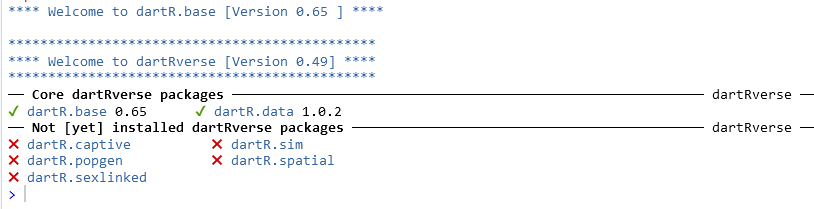
\includegraphics{images/dartRverse.png} \hfill{}

\end{figure}

\hypertarget{install-additional-packages}{%
\subsection*{install additional
packages}\label{install-additional-packages}}
\addcontentsline{toc}{subsection}{install additional packages}

Now we can install the additional packages that are part of the
dartRverse. Depending on your needs you can install all of them or only
the one you are interested.

For example if you are interested in additional functions to analyse
population structure (e.g.~run STRUCTURE or faststructure) you can
install the dartR.popgen package. If you are interested in functions
that support the simulation of data you can install the dartR.sim
package.

You can check which packages are avaialbel and which of them you have
installed by typing:

\begin{Shaded}
\begin{Highlighting}[]
\NormalTok{dartRverse}\SpecialCharTok{::}\FunctionTok{dartRverse\_install}\NormalTok{()}
\end{Highlighting}
\end{Shaded}

\begin{figure}

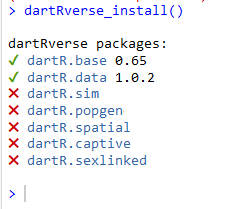
\includegraphics{images/dartRverse_install.png} \hfill{}

\end{figure}

The currently available packages are:

\begin{itemize}
\tightlist
\item
  dartR.sim (simulate SNP data)
\item
  dartR.popgen (run population genetic analysis)
\item
  dartR.spatial (run landscape genetic analysis)
\item
  dartR.captive (estimate relatedness, support captive breeding)
\item
  dartR.sexlinked (identify sexlinked markers, not ready yet)
\end{itemize}

So to install the dartR.sim simply type:

\begin{Shaded}
\begin{Highlighting}[]
\FunctionTok{install.packages}\NormalTok{(}\StringTok{"dartR.sim"}\NormalTok{)}
\end{Highlighting}
\end{Shaded}

\hypertarget{github-repositories}{%
\subsection*{Github repositories}\label{github-repositories}}
\addcontentsline{toc}{subsection}{Github repositories}

We make all of our packages available via CRAN. The reason for this is
that CRAN packages follow a stringent testing before they are allowed to
be uploaded to CRAN and therefore are more likely to contain less errors
then packages that are available on other repositories. Nevertheless we
also make our packages available during development via github.

You can find the repositories under:
\url{https://github.com/green-striped-gecko/dartR.base} {[}for the
dartR.base package{]} and equivalent for the other packages.

The reason why you might want to install a package from github is that
you want to use the latest version of the package. However, you should
be aware that the packages on github are not tested and therefore might
contain errors. Also the packages on github might be updated on a daily
basis and therefore might change without notice.

We use different branches and they are reflecting different stages of
development and majurity.

\begin{itemize}
\tightlist
\item
  main (the main branch, which is equivalent to the current CRAN
  version)
\item
  dev (development branch, which has the latest functions that might be
  in the next CRAN version, but have not been tested yet)
\item
  dev\_name (these are branches of our main developers and are used for
  testing and development of new functions. Installing functions from
  here might cause problems and should only be done if you know what you
  are doing)
\end{itemize}

dartRverse supports the installation of github version of the packages
using the following syntax:

\texttt{dartRverse\_install(package\ =\ "dartR.base,\ repo\ =\ "github",\ branch\ =\ "dev")}

This install the dev branch of dartR.base from CRAN. All main and dev
branches are tested if they can be installed (and some additional error
checks via): \url{https://github.com/green-striped-gecko/dartRverse}

Please note that you should provide the package repository
(github/cran), the branch (main, dev,dev\_name) and version number in
case you want to report a bug. You can use the github methods to report
issues or use our google group:
\url{https://groups.google.com/d/forum/dartr}.

\hypertarget{using-legacy-dartr}{%
\section*{Using legacy dartR}\label{using-legacy-dartr}}
\addcontentsline{toc}{section}{Using legacy dartR}

\markright{Using legacy dartR}

For whatever reason you might want to use legacy dartR, instead of the
dartRverse packages {[}e.g.~for initial testing{]}. The good news is
that both packages can be installed next to each other, but you need to
make sure you detach the other package. This can be done in Rstudio via
the package tab by unticking the packages. Please note the order you
unclick packages is important. So first the non-core packages
(dartR.sim, dartR.popgen, dartR.captive, dartR.spatial), then dartRverse
followed by the core packages dartR.base and finally dartR.data. If you
do not follow the correct order you get a warning message and it will
not detach the package. If you want to use code type:

\begin{Shaded}
\begin{Highlighting}[]
\FunctionTok{detach}\NormalTok{(}\StringTok{"package:dartR.sim"}\NormalTok{, }\AttributeTok{unload =} \ConstantTok{TRUE}\NormalTok{)}
\FunctionTok{detach}\NormalTok{(}\StringTok{"package:dartR.sexlinked"}\NormalTok{, }\AttributeTok{unload =} \ConstantTok{TRUE}\NormalTok{)}
\FunctionTok{detach}\NormalTok{(}\StringTok{"package:dartR.spatial"}\NormalTok{, }\AttributeTok{unload =} \ConstantTok{TRUE}\NormalTok{)}
\FunctionTok{detach}\NormalTok{(}\StringTok{"package:dartR.captive"}\NormalTok{, }\AttributeTok{unload =} \ConstantTok{TRUE}\NormalTok{)}
\FunctionTok{detach}\NormalTok{(}\StringTok{"package:dartR.popgen"}\NormalTok{, }\AttributeTok{unload =} \ConstantTok{TRUE}\NormalTok{)}
\FunctionTok{detach}\NormalTok{(}\StringTok{"package:dartRverse"}\NormalTok{, }\AttributeTok{unload =} \ConstantTok{TRUE}\NormalTok{)}
\FunctionTok{detach}\NormalTok{(}\StringTok{"package:dartR.base"}\NormalTok{, }\AttributeTok{unload =} \ConstantTok{TRUE}\NormalTok{)}
\FunctionTok{detach}\NormalTok{(}\StringTok{"package:dartR.data"}\NormalTok{, }\AttributeTok{unload =} \ConstantTok{TRUE}\NormalTok{)}
\end{Highlighting}
\end{Shaded}

Now you can load the legacy dartR package and use it as before.

\begin{Shaded}
\begin{Highlighting}[]
\FunctionTok{library}\NormalTok{(dartR)}
\end{Highlighting}
\end{Shaded}

To unload dartR you can use the Packages tab as described before or the
following code:

\begin{Shaded}
\begin{Highlighting}[]
\FunctionTok{detach}\NormalTok{(}\StringTok{"package:dartR"}\NormalTok{, }\AttributeTok{unload =} \ConstantTok{TRUE}\NormalTok{)}
\FunctionTok{detach}\NormalTok{(}\StringTok{"package:dartR.data"}\NormalTok{, }\AttributeTok{unload =} \ConstantTok{TRUE}\NormalTok{)}
\end{Highlighting}
\end{Shaded}

\hypertarget{using-dartrverse}{%
\section*{using dartRverse}\label{using-dartrverse}}
\addcontentsline{toc}{section}{using dartRverse}

\markright{using dartRverse}

To use dartRverse you can simply load the package and use it as before.

\begin{Shaded}
\begin{Highlighting}[]
\FunctionTok{library}\NormalTok{(dartRverse)}
\end{Highlighting}
\end{Shaded}

\bookmarksetup{startatroot}

\hypertarget{basic-filtering}{%
\chapter*{Basic filtering}\label{basic-filtering}}
\addcontentsline{toc}{chapter}{Basic filtering}

\markboth{Basic filtering}{Basic filtering}

by Arthur Georges, Bernd Gruber \& Luis Mijangos

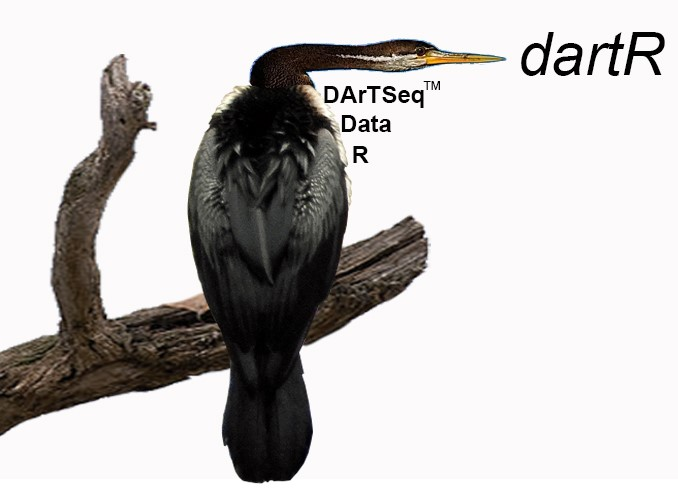
\includegraphics[width=1.875in,height=\textheight]{images/logo_old.jpg}
\newpage

\hypertarget{session-1-basic-filtering}{%
\section*{Session 1: Basic Filtering}\label{session-1-basic-filtering}}
\addcontentsline{toc}{section}{Session 1: Basic Filtering}

\markright{Session 1: Basic Filtering}

\hypertarget{overview}{%
\subsection*{Overview}\label{overview}}
\addcontentsline{toc}{subsection}{Overview}

Calling SNPs in genotyping by sequencing is not an exact science.
Judgements need to be made at various points in the workflow to increase
the likelihood of a correct call at a particular locus. Diversity Arrays
Pty Ltd (DArT) has already done much of the filtering of the sequences
used to generate your SNPs that would normally be undertaken by
researchers who generate their own ddRAD data. Here we present some
other filters that you might wish to apply to increase the reliability
of the data retained in your SNP or SilicoDArT dataset. For each filter
parameter offered by dartR, we provide both a report function and a
filtering function (e.g.~gl.report.reproducibility us associated with
\texttt{gl.filter.reproducability}). The reporting function provides
descriptive statistics for the parameter of choice. Inspection of these
outputs will assist you to identify appropriate filter thresholds.
Hence, as a standard workflow, it is a good idea to run the gl.report
functions in advance of applying each gl.filter function to provide a
foundation for selecting thresholds. Several filters are available to
improve the quality of the data represented in your genlight object.
Some of these are specific to Diversity Arrays data
(e.g.~\texttt{gl.filter.reproducibility}), but most will work on any
data provided they are in the appropriate genlight format. The basic
ones, in no particular order, are:

\begin{longtable}[]{@{}
  >{\raggedright\arraybackslash}p{(\columnwidth - 2\tabcolsep) * \real{0.5000}}
  >{\raggedright\arraybackslash}p{(\columnwidth - 2\tabcolsep) * \real{0.5000}}@{}}
\toprule\noalign{}
\endhead
\bottomrule\noalign{}
\endlastfoot
\texttt{gl\ \textless{}-\ gl.filter.reproducibility()} & filter out loci
for which the reproducibility (strictly repeatability) is less than a
specified threshold, say threshold = 0.99 \\
\texttt{gl\ \textless{}-\ gl.filter.callrate()} & filter out loci or
individuals for which the call rate (rate of non-missing values) is less
than a specified threshold, say threshold = 0.95 \\
\texttt{gl\ \textless{}-\ gl.filter.monomorphs()} & filter out
monomorphic loci and loci that are scored all NA \\
\texttt{gl\ \textless{}-\ gl.filter.allna} & filter out loci that are
all missing values (NA) \\
\texttt{gl\ \textless{}-gl.filter.secondaries()} & filter out SNPs that
share a sequence tag, except one retained at random {[}or the best based
on reproducibility (RepAvg) and information content (AvgPIC){]} \\
\texttt{gl\ \textless{}-\ gl.filter.hamming()} & filter out loci that
differ from each other by less than a specified number of base pairs \\
\texttt{gl\ \textless{}-\ gl.filter.rdepth()} & filter out loci with
exceptionally low or high read depth (coverage) \\
\texttt{gl\ \textless{}-\ gl.filter.taglength()} \textbar filter out
loci for which the tag length is less that a threshold \textbar{} & \\
\texttt{gl\ \textless{}-\ gl.filter.overshoot()} \textbar{} filter out
loci where the SNP location lies outside the trimmed sequence tag
\textbar{} & \\
\end{longtable}

The order of filtering can be important and requires some thought. As an
example, filtering on call rate by individual before filtering on call
rate by locus or choosing the alternative order will depend on the
weight placed on losing individuals versus losing loci. The filtering
steps may also change depending on the analysis you intend to run. There
is no one-fits-all approach to SNP filtering.

\hypertarget{filtering-on-reproducibility}{%
\subsection*{Filtering on
reproducibility}\label{filtering-on-reproducibility}}
\addcontentsline{toc}{subsection}{Filtering on reproducibility}

As an additional quality control, a selection of samples is processed
twice by Diversity Arrays Technology using independent adaptors from DNA
through to allelic calls. Scoring consistency of these technical
replicates is referred to as reproducibility. Let's examine the
distribution of reproducibility measures (RepAvg) in our dataset.

Loading the package (assuming you have installed dartRverse - see
chapter dartRverse)

\begin{Shaded}
\begin{Highlighting}[]
\FunctionTok{library}\NormalTok{(dartRverse)}
\end{Highlighting}
\end{Shaded}

\subsubsection{code}

\begin{Shaded}
\begin{Highlighting}[]
\FunctionTok{gl.report.reproducibility}\NormalTok{(testset.gl , }\AttributeTok{verbose =} \DecValTok{1}\NormalTok{)}
\end{Highlighting}
\end{Shaded}

\subsubsection{output}

\begin{verbatim}
Starting gl.report.reproducibility 
  Reporting Repeatability by Locus
  No. of loci = 255 
  No. of individuals = 250 
    Minimum      :  0.959459 
    1st quartile :  1 
    Median       :  1 
    Mean         :  0.9981525 
    3r quartile  :  1 
    Maximum      :  1 
    Missing Rate Overall:  0.12 
\end{verbatim}

\includegraphics{basicfiltering_files/figure-pdf/unnamed-chunk-3-1.pdf}

\begin{verbatim}
   Quantile Threshold Retained Percent Filtered Percent
1      100%  1.000000      214    83.9       41    16.1
2       95%  1.000000      214    83.9       41    16.1
3       90%  1.000000      214    83.9       41    16.1
4       85%  1.000000      214    83.9       41    16.1
5       80%  1.000000      214    83.9       41    16.1
6       75%  1.000000      214    83.9       41    16.1
7       70%  1.000000      214    83.9       41    16.1
8       65%  1.000000      214    83.9       41    16.1
9       60%  1.000000      214    83.9       41    16.1
10      55%  1.000000      214    83.9       41    16.1
11      50%  1.000000      214    83.9       41    16.1
12      45%  1.000000      214    83.9       41    16.1
13      40%  1.000000      214    83.9       41    16.1
14      35%  1.000000      214    83.9       41    16.1
15      30%  1.000000      214    83.9       41    16.1
16      25%  1.000000      214    83.9       41    16.1
17      20%  1.000000      214    83.9       41    16.1
18      15%  0.997674      217    85.1       38    14.9
19      10%  0.994536      230    90.2       25     9.8
20       5%  0.984694      243    95.3       12     4.7
21       0%  0.959459      255   100.0        0     0.0
Completed: gl.report.reproducibility 
\end{verbatim}

We now filter on selecting a threshold value of 0.99.

\subsubsection{code}

\begin{Shaded}
\begin{Highlighting}[]
\NormalTok{gl }\OtherTok{\textless{}{-}} \FunctionTok{gl.filter.reproducibility}\NormalTok{( testset.gl, }\AttributeTok{threshold=}\FloatTok{0.99}\NormalTok{, }\AttributeTok{verbose =} \DecValTok{1}\NormalTok{)}
\end{Highlighting}
\end{Shaded}

\subsubsection{output}

\begin{verbatim}
Starting gl.select.colors 
  Warning: Number of required colors not specified, set to 9
  Library: RColorBrewer
  Palette: brewer.pal
  Showing and returning 2 of 9 colors for library RColorBrewer : palette Blues 
\end{verbatim}

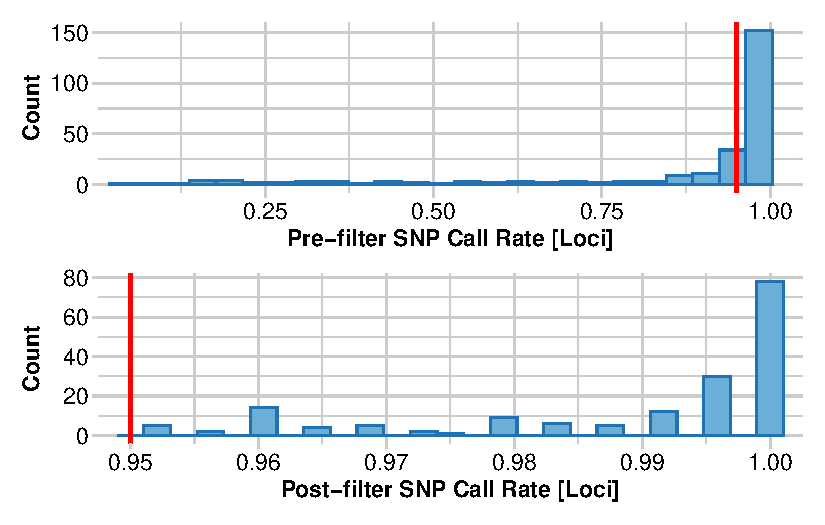
\includegraphics{basicfiltering_files/figure-pdf/unnamed-chunk-5-1.pdf}

\begin{verbatim}
Completed: gl.select.colors 
Starting gl.filter.reproducibility 
\end{verbatim}

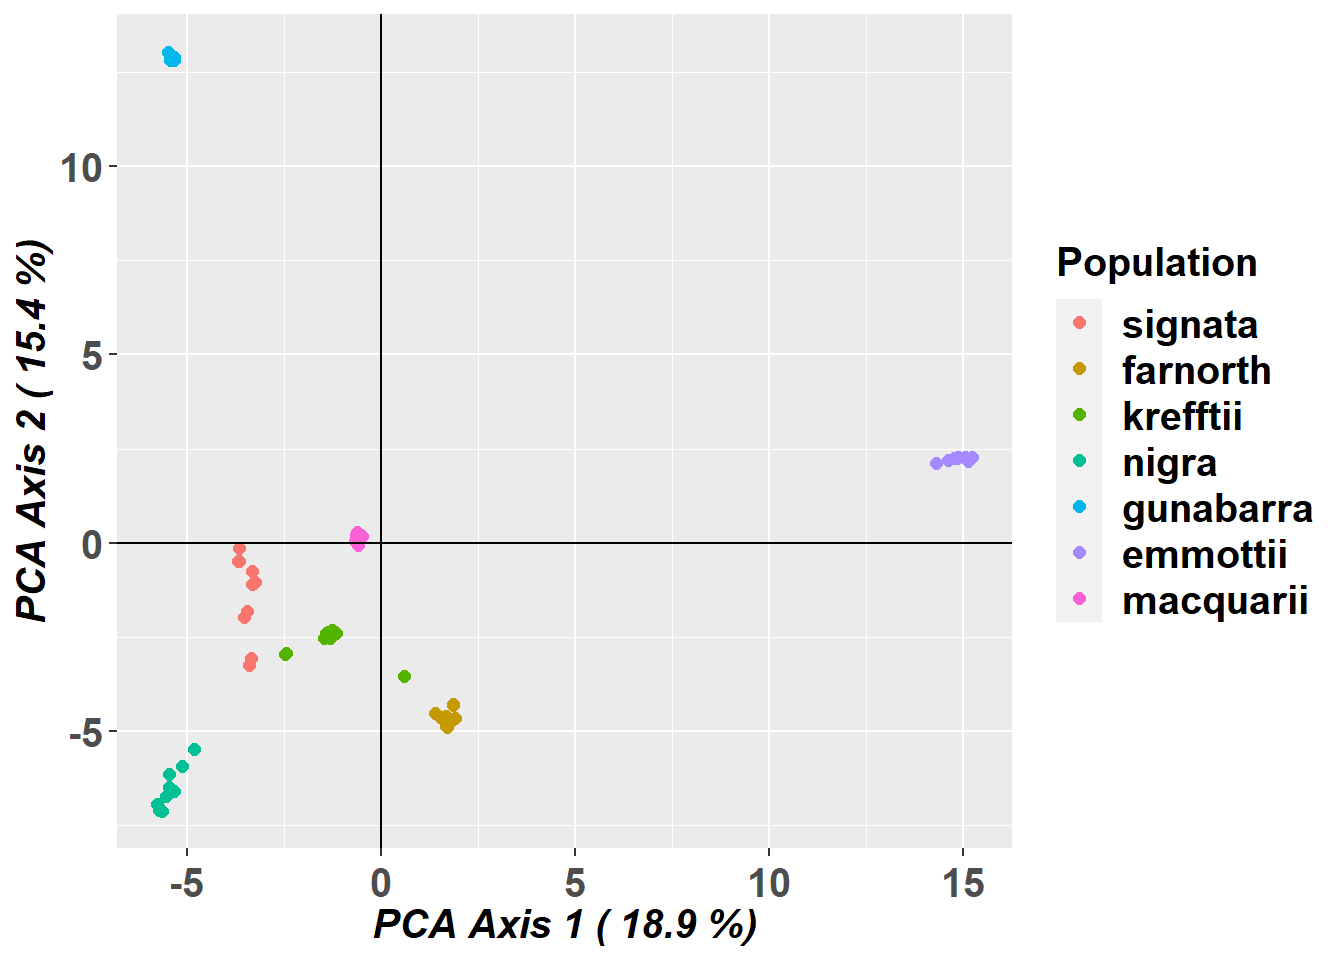
\includegraphics{basicfiltering_files/figure-pdf/unnamed-chunk-5-2.pdf}

\begin{verbatim}
Completed: gl.filter.reproducibility 
\end{verbatim}

Only 14 loci out of 255 were removed.

\begin{tcolorbox}[enhanced jigsaw, coltitle=black, colframe=quarto-callout-note-color-frame, colbacktitle=quarto-callout-note-color!10!white, breakable, bottomtitle=1mm, rightrule=.15mm, opacitybacktitle=0.6, left=2mm, arc=.35mm, opacityback=0, leftrule=.75mm, toptitle=1mm, titlerule=0mm, title=\textcolor{quarto-callout-note-color}{\faInfo}\hspace{0.5em}{Exercise}, bottomrule=.15mm, toprule=.15mm, colback=white]


\includegraphics[width=0.5in,height=0.5in]{images/task.png}

\begin{enumerate}
\def\labelenumi{\arabic{enumi}.}
\item
  Just in case you have accidentally modified the genlight object gl,
  recreate it by copying it from \texttt{testset.gl}.

  \texttt{gl\ \textless{}-\ testset.gl}
\item
  Filter gl using the filters listed above. Request a report first to
  inform your choice of threshold. Be sure to set plot=TRUE to examine
  the distribution of each parameter and optionally
  \texttt{smearplot=TRUE} to examine the smear plot.
\end{enumerate}

\end{tcolorbox}

\hypertarget{filtering-on-call-rate}{%
\subsection*{Filtering on call rate}\label{filtering-on-call-rate}}
\addcontentsline{toc}{subsection}{Filtering on call rate}

A filter for Call Rate can be applied to loci and to individuals. When
filtering on loci, only those for which the associated SNP is called in
at least a specified proportion will be retained. When filtering on
individuals, only those individuals for which a specified percentage of
loci are scored for a SNP polymorphism will be retained.

\textbf{Filtering on Loci}

Recall that Call Rate for SNPs can arise from two sources. The first
source is where a missing value arises because the sequence tag bearing
the target SNP cannot be amplified -- there has been a mutation at one
or both of the restriction sites. The second source of missing values is
where the read depth is insufficient to make a reliable call on the SNP.
Either way, the SNP is not called and is recorded as NA. For
presence-absence data (i.e.~SilicoDArT), the sequence tag is recorded as
having been amplified (presence) or not (absence). A missing value
arises when it is not possible to determine if the sequence tag has been
amplified or not, so in that sense it is true missing data. A first step
in filtering on Call Rate is to examine the distribution of Call Rates
across loci. We use the function \texttt{gl.report.callrate} to yield
the following output and graph.

\begin{Shaded}
\begin{Highlighting}[]
\FunctionTok{gl.report.callrate}\NormalTok{(testset.gl)}
\end{Highlighting}
\end{Shaded}

\begin{verbatim}
Starting gl.report.callrate 
  Processing genlight object with SNP data
  Reporting Call Rate by Locus
  No. of loci = 255 
  No. of individuals = 250 
    Minimum      :  0.056 
    1st quartile :  0.912 
    Median       :  0.984 
    Mean         :  0.8765804 
    3r quartile  :  1 
    Maximum      :  1 
    Missing Rate Overall:  0.1234 
\end{verbatim}

\begin{figure}[H]

{\centering 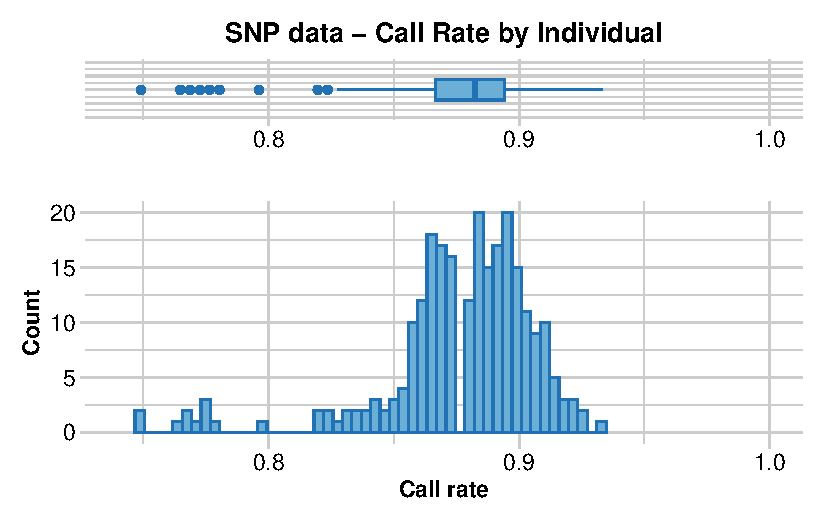
\includegraphics{basicfiltering_files/figure-pdf/unnamed-chunk-6-1.pdf}

}

\end{figure}

\begin{verbatim}
Completed: gl.report.callrate 
\end{verbatim}

Here you can see that the call rate for most loci is close to 100\%, but
that there is a tail of loci for which the call rate is exceptionally
poor. In this case, we might choose to filter out loci for which the
call rate is less than 95\% (0.95).

\begin{Shaded}
\begin{Highlighting}[]
\NormalTok{gl }\OtherTok{\textless{}{-}} \FunctionTok{gl.filter.callrate}\NormalTok{(testset.gl, }\AttributeTok{threshold=}\FloatTok{0.95}\NormalTok{)}
\end{Highlighting}
\end{Shaded}

\begin{verbatim}
Starting gl.filter.callrate 
  Processing genlight object with SNP data
  Warning: Data may include monomorphic loci in call rate 
                    calculations for filtering
  Recalculating Call Rate
  Removing loci based on Call Rate, threshold = 0.95 
\end{verbatim}

\begin{figure}[H]

{\centering \includegraphics{basicfiltering_files/figure-pdf/unnamed-chunk-7-1.pdf}

}

\end{figure}

\begin{verbatim}
Completed: gl.filter.callrate 
\end{verbatim}

The results of the filtering are shown as a before-after plot. For most
purposes, this filtering of poorly called loci is likely to be
satisfactory.

\textbf{Filtering on Individuals}

A second way of filtering on Call Rate is to remove individuals that
have sequenced particularly poorly. This may occur if the associated
samples are degraded in comparison with other samples. We again first
report the Call Rate, this time for individuals.

\begin{Shaded}
\begin{Highlighting}[]
\FunctionTok{gl.report.callrate}\NormalTok{(testset.gl, }\AttributeTok{method=}\StringTok{\textquotesingle{}ind\textquotesingle{}}\NormalTok{)}
\end{Highlighting}
\end{Shaded}

\begin{verbatim}
Starting gl.report.callrate 
  Processing genlight object with SNP data

  Reporting Call Rate by Individual
  No. of loci = 255 
  No. of individuals = 250 
    Minimum      :  0.7490196 
    1st quartile :  0.8666667 
    Median       :  0.8823529 
    Mean         :  0.8765804 
    3r quartile  :  0.8941176 
    Maximum      :  0.9333333 
    Missing Rate Overall:  0.1234 

Listing 30 populations and their average CallRates
  Monitor again after filtering
         Population CallRate  N
1     EmmacBrisWive   0.8839 10
2     EmmacBurdMist   0.8808 10
3     EmmacBurnBara   0.8859 11
4     EmmacClarJack   0.8596  5
5     EmmacClarYate   0.8769  5
6     EmmacCoopAvin   0.7682 10
7    EmmacCoopCully   0.9122 10
8     EmmacCoopEulb   0.8702 10
9    EmmacFitzAllig   0.8973 10
10    EmmacJohnWari   0.8929 10
11    EmmacMaclGeor   0.8806 11
12    EmmacMaryBoru   0.8843  6
13    EmmacMaryPetr   0.8892  4
14     EmmacMDBBowm   0.8824 10
15     EmmacMDBCond   0.8855 10
16     EmmacMDBCudg   0.8878 10
17     EmmacMDBForb   0.8766 11
18     EmmacMDBGwyd   0.9050  9
19     EmmacMDBMaci   0.8773 10
20 EmmacMDBMurrMung   0.8890 10
21     EmmacMDBSanf   0.8914 10
22    EmmacNormJack   0.8725  6
23    EmmacNormLeic   0.8863  1
24    EmmacNormSalt   0.8706  1
25    EmmacRichCasi   0.8757 10
26        EmmacRoss   0.8706 10
27    EmmacRussEube   0.8612 10
28     EmmacTweeUki   0.8773 10
29    EmsubRopeMata   0.8345  5
30    EmvicVictJasp   0.8361  5

Listing 20 individuals with the lowest CallRates
  Use this list to see which individuals will be lost on filtering by individual
  Set ind.to.list parameter to see more individuals
   Individual  CallRate
1    AA063722 0.7490196
2    AA063726 0.7490196
3    AA063732 0.7647059
4    AA063720 0.7686275
5    AA063712 0.7686275
6    AA063708 0.7725490
7    AA063718 0.7764706
8    AA063710 0.7764706
9    AA063714 0.7764706
10   AA063716 0.7803922
11   AA032760 0.7960784
12   UC_00210 0.8196078
13   UC_00259 0.8196078
14   AA018494 0.8235294
15   UC_00206 0.8235294
16   AA019164 0.8274510
17   UC_00209 0.8313725
18   UC_00254 0.8313725
19   AA019159 0.8352941
20  UC_00126c 0.8352941

)
\end{verbatim}

\begin{figure}[H]

{\centering 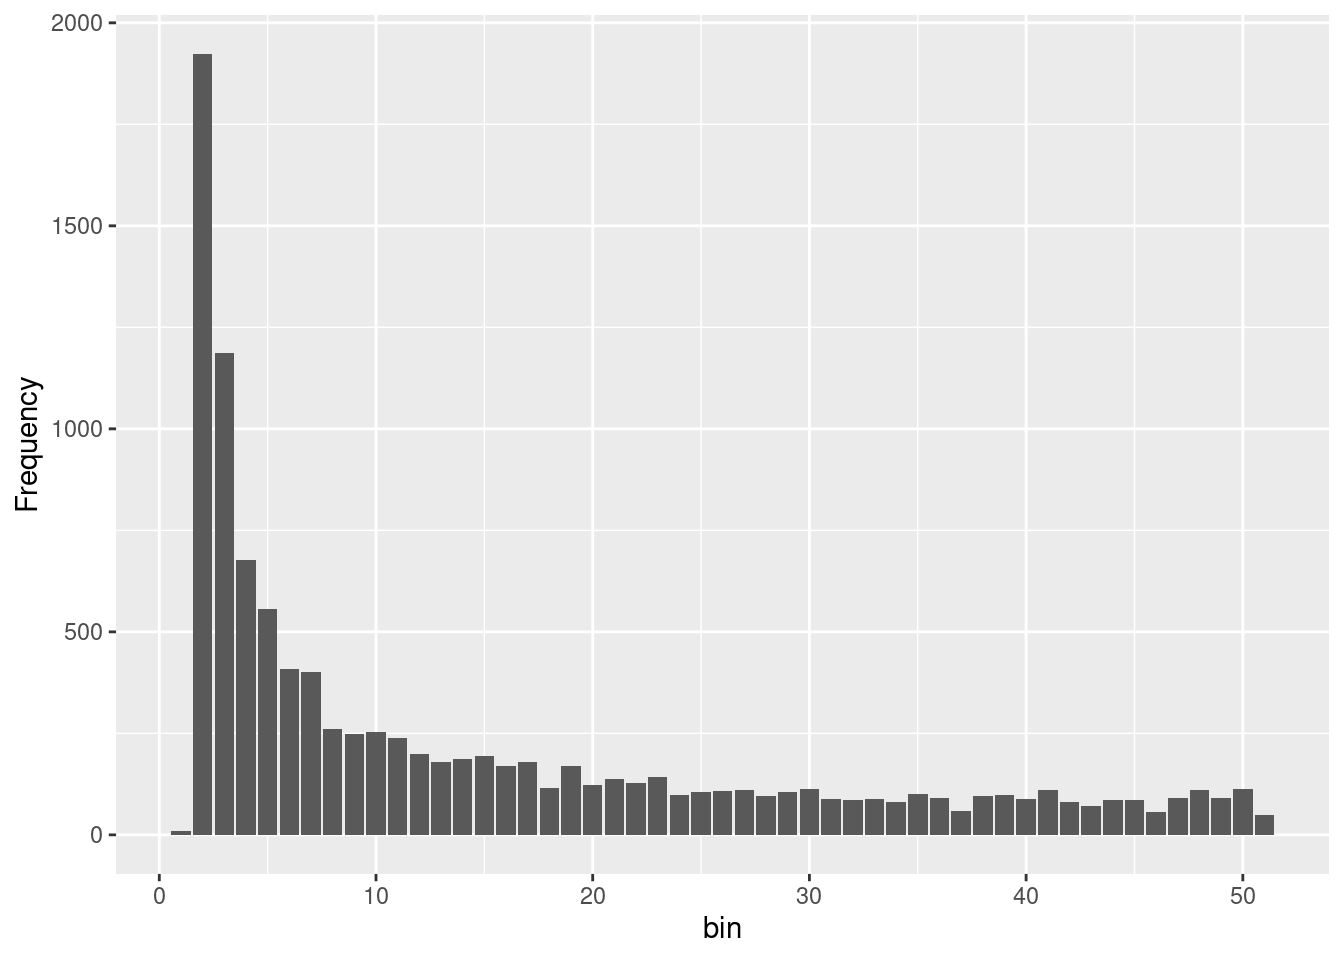
\includegraphics{basicfiltering_files/figure-pdf/unnamed-chunk-8-1.pdf}

}

\end{figure}

\begin{verbatim}
Completed: gl.report.callrate 
\end{verbatim}

The output will include a list of populations and the Call Rate averaged
across individuals, and a list of the top worst individuals in terms of
their call rate. This will allow you to make a reasoned judgement on the
impact of filtering out individuals. The graph tells the story. In the
absence of information to the contrary, a threshold of 80\% (0.80) would
seem appropriate for filtering individuals on Call Rate.

We execute the filter with a threshold of 0.80.

\begin{Shaded}
\begin{Highlighting}[]
\NormalTok{gl }\OtherTok{\textless{}{-}} \FunctionTok{gl.filter.callrate}\NormalTok{(testset.gl, }\AttributeTok{threshold=}\FloatTok{0.80}\NormalTok{, }\AttributeTok{method=}\StringTok{\textquotesingle{}ind\textquotesingle{}}\NormalTok{)}
\end{Highlighting}
\end{Shaded}

\begin{verbatim}
Starting gl.filter.callrate 
  Processing genlight object with SNP data
  Warning: Data may include monomorphic loci in call rate 
                    calculations for filtering
  Recalculating Call Rate
  Removing individuals based on Call Rate, threshold = 0.8 
  Individuals deleted (CallRate <=  0.8 ):
AA032760[EmmacMDBMaci], AA063718[EmmacCoopAvin], AA063720[EmmacCoopAvin], AA063722[EmmacCoopAvin], AA063726[EmmacCoopAvin], AA063732[EmmacCoopAvin], AA063708[EmmacCoopAvin], AA063710[EmmacCoopAvin], AA063712[EmmacCoopAvin], AA063714[EmmacCoopAvin], AA063716[EmmacCoopAvin],
\end{verbatim}

\begin{figure}[H]

{\centering 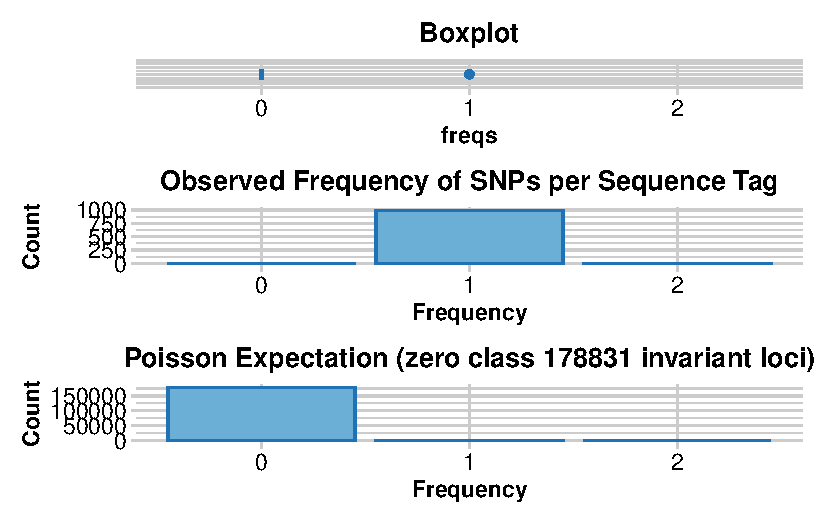
\includegraphics{basicfiltering_files/figure-pdf/unnamed-chunk-9-1.pdf}

}

\end{figure}

\begin{verbatim}
  Note: Locus metrics not recalculated
  Note: Resultant monomorphic loci not deleted
Completed: gl.filter.callrate 
\end{verbatim}

This statement filters out individuals with a Call Rate across loci of
less than 80\%. It conveniently lists the individuals that have been
removed and the populations to which they belong so you can assess the
impact of the filtering.

\hypertarget{filter-seconaries}{%
\subsection*{Filter Seconaries}\label{filter-seconaries}}
\addcontentsline{toc}{subsection}{Filter Seconaries}

Sequence tags can contain more than one callable SNP marker. Because of
their close proximity, these multiple SNPs within a single sequence tag
(referred to in dartR as `secondaries' are likely to be strongly linked
(inherited together). This is problematic for many analyses, so one
might wish to filter out the multiple SNPs to leave only one per
sequence tag. Diversity Arrays Technology include multiple SNPS in a
single sequence tag each as separate records in the data provided with
your report. The decision becomes, which SNP to retain, and which SNPs
to discard. One strategy is to leave the filtering of secondaries until
last, so that you are considering only those secondaries that have
survived the earlier filtering on call rate, reproducibility and read
depth. You can then choose one from the surviving secondaries at random
(method=`random') or based on comparisons of reproducibility (RepAvg)
and polymorphism information content (PIC) (method=`best'). The call is:

\begin{Shaded}
\begin{Highlighting}[]
\FunctionTok{gl.report.secondaries}\NormalTok{(gl)}
\end{Highlighting}
\end{Shaded}

\begin{verbatim}
Starting gl.report.secondaries 
  Processing genlight object with SNP data
Counting ....
  Warning: No loci with secondaries, no plot produced
  Total number of SNP loci scored: 255 
    Number of secondaries: 0 
Completed: gl.report.secondaries 
\end{verbatim}

\begin{verbatim}
               Param       Value
1       n.total.tags   255.00000
2 n.SNPs.secondaries     0.00000
3   n.invariant.tags          NA
4 n.tags.secondaries          NA
5          n.inv.gen 15224.00000
6       mean.len.tag    60.70196
7        n.invariant          NA
8             Lambda          NA
\end{verbatim}

The output is a bit more complex than one might expect. The total number
of SNPs scored in the dataset gl is 119,414 residing on 70,942 sequence
tags. So there are many sequence tags with more than one SNP (indeed
28,769). Filtering on secondaries will remove 48,477 SNPs. The function
models the frequency spectrum of SNPs per sequence tag with a zero
truncated Poisson Distribution (strictly the distribution is a compound
Poisson as lamda varies) and uses that distribution to estimate the
unknown zero class -- the number of sequence tags expected to contain no
SNP (that is, the invariant sequence tags). This value of 7,317,732 can
be used to correct the denominator for estimates of heterozygosity.

This estimation is best shown in a graph. (Knuth 1984: the original
example with gl does not give a plot)

\begin{Shaded}
\begin{Highlighting}[]
\FunctionTok{gl.report.secondaries}\NormalTok{(bandicoot.gl, }\AttributeTok{verbose=}\DecValTok{1}\NormalTok{)}
\end{Highlighting}
\end{Shaded}

\begin{verbatim}
Starting gl.report.secondaries 
The column 'TrimmedSequence' was not found in loc.metrics
 Mean tag length assumed to be 69 
\end{verbatim}

\begin{figure}[H]

{\centering \includegraphics{basicfiltering_files/figure-pdf/unnamed-chunk-11-1.pdf}

}

\end{figure}

\begin{verbatim}
  Total number of SNP loci scored: 1000 
   Number of sequence tags in total: 999 
   Estimated number of invariant sequence tags: 178831 
   Number of sequence tags with secondaries: 1 
   Number of secondary SNP loci that would be removed on 
            filtering: 1 
   Number of SNP loci that would be retained on filtering: 999 
   Number of invariant sites in sequenced tags: 67931 
   Mean length of sequence tags: 69 
   Total Number of invariant sites (including invariant sequence 
            tags): 12407270 
Completed: gl.report.secondaries 
\end{verbatim}

\begin{verbatim}
               Param        Value
1       n.total.tags 9.990000e+02
2 n.SNPs.secondaries 1.000000e+00
3   n.invariant.tags 1.788310e+05
4 n.tags.secondaries 1.000000e+00
5          n.inv.gen 6.793100e+04
6       mean.len.tag 6.900000e+01
7        n.invariant 1.240727e+07
8             Lambda 5.570726e-03
\end{verbatim}

Note that the estimate of the zero class involves an iterative process
that does not always converge to a satisfactory solution for lamda. In
this case it did. Note also that the estimate of the zero class can have
a very substantial error associated with it, especially if the count for
class 0 exceeds the count for the class 1. Useful, but not infallible.
Having examined the report, filtering out the secondaries is done using

\begin{Shaded}
\begin{Highlighting}[]
\NormalTok{gl }\OtherTok{\textless{}{-}} \FunctionTok{gl.filter.secondaries}\NormalTok{(gl,}\AttributeTok{method=}\StringTok{"random"}\NormalTok{)}
\end{Highlighting}
\end{Shaded}

\begin{verbatim}
Starting gl.filter.secondaries 
  Processing genlight object with SNP data
  Selecting one SNP per sequence tag at random
Completed: gl.filter.secondaries 
\end{verbatim}

\hypertarget{filtering-on-hamming-distance}{%
\subsection*{filtering on Hamming
Distance}\label{filtering-on-hamming-distance}}
\addcontentsline{toc}{subsection}{filtering on Hamming Distance}

Hamming distance is a measure of sequence similarity between sequence
tags. If two sequence tags (69 bp) differ by only a couple of base pairs
then suspicion is aroused as to whether they have arisen by sequencing
error. Diversity Arrays Technology have already filtered on a Hamming
distance of 3 bp. Rarely you might want to go further, and the
\texttt{gl.filter.hamming} function gives you this option.

\begin{Shaded}
\begin{Highlighting}[]
\NormalTok{gl }\OtherTok{\textless{}{-}} \FunctionTok{gl.filter.hamming}\NormalTok{(testset.gl)}
\end{Highlighting}
\end{Shaded}

\begin{verbatim}
Starting gl.filter.hamming 
  Processing genlight object with SNP data
  Filtering loci with a Hamming Distance of less than 0.2 
\end{verbatim}

\begin{figure}[H]

{\centering 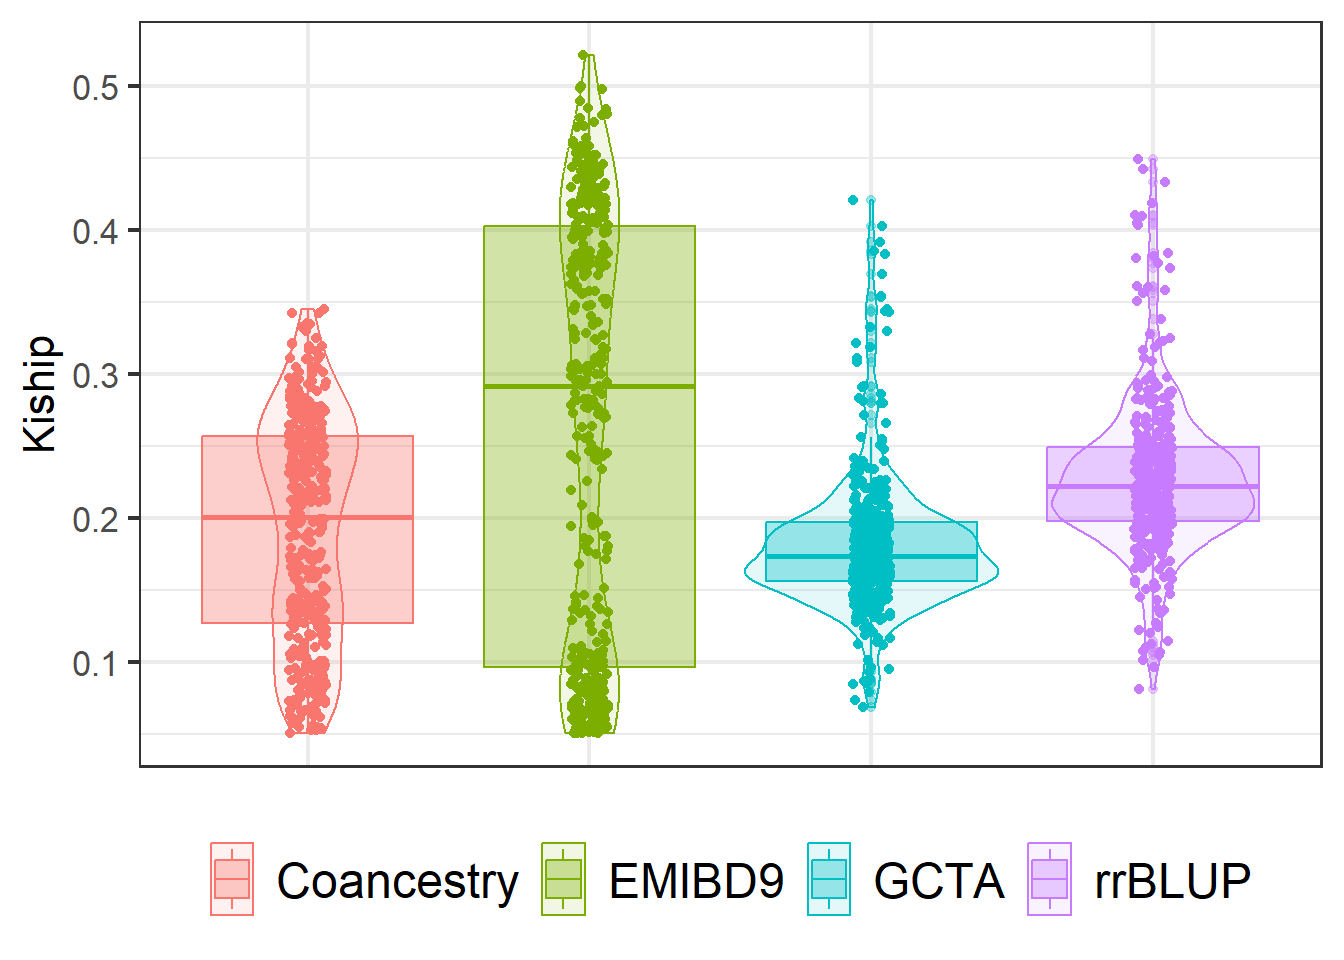
\includegraphics{basicfiltering_files/figure-pdf/unnamed-chunk-13-1.pdf}

}

\end{figure}

\begin{verbatim}
Completed: gl.filter.hamming 
\end{verbatim}

\begin{tcolorbox}[enhanced jigsaw, coltitle=black, colframe=quarto-callout-note-color-frame, colbacktitle=quarto-callout-note-color!10!white, breakable, bottomtitle=1mm, rightrule=.15mm, opacitybacktitle=0.6, left=2mm, arc=.35mm, opacityback=0, leftrule=.75mm, toptitle=1mm, titlerule=0mm, title=\textcolor{quarto-callout-note-color}{\faInfo}\hspace{0.5em}{Exercise}, bottomrule=.15mm, toprule=.15mm, colback=white]


\includegraphics[width=0.5in,height=0.5in]{images/task.png} Try this for
yourself on genlight object gl after filtering or on your own data

\end{tcolorbox}

Similarly, when filtering has resulted in removal of some individuals or
populations, variation at several loci may be lost. Some loci may even
be scored as missing across all individuals. You may wish to remove
these monomorphic loci from your dataset with

\texttt{gl\ \textless{}-\ gl.filter.monomorphs(gl)}

\begin{tcolorbox}[enhanced jigsaw, coltitle=black, colframe=quarto-callout-note-color-frame, colbacktitle=quarto-callout-note-color!10!white, breakable, bottomtitle=1mm, rightrule=.15mm, opacitybacktitle=0.6, left=2mm, arc=.35mm, opacityback=0, leftrule=.75mm, toptitle=1mm, titlerule=0mm, title=\textcolor{quarto-callout-note-color}{\faInfo}\hspace{0.5em}{Exercise}, bottomrule=.15mm, toprule=.15mm, colback=white]


\includegraphics[width=0.5in,height=0.5in]{images/task.png} Try this for
yourself on genlight object gl after filtering or on your own data

\end{tcolorbox}

Note that many functions have a \texttt{mono.rm} and \texttt{recalc}
parameters that allow you to remove monomorphic loci or recalculate
metrics on the fly. It is not a fatal error to forget to recalculate the
locus metrics because dartR scripts will detect if they have not been
recalculated and rectify this before they a particular locus metric is
needed.

\hypertarget{where-have-we-come}{%
\subsection*{Where have we come?}\label{where-have-we-come}}
\addcontentsline{toc}{subsection}{Where have we come?}

The above Session was designed to give you an overview of the scripts in
dartR for filtering your data. Having completed this Session, you should
now able to:

\begin{itemize}
\tightlist
\item
  Filter on call rate, reproducibility, secondaries, read depth and
  hamming distance.
\item
  Recalculate locus metrics after deleting individuals or populations as
  part of the filtering process.
\item
  Filter out resultant monomorphic loci.
\end{itemize}

Having played with the various filters, you should also have a good
appreciation of how to use the \texttt{gl.report} functions to select
appropriate thresholds for filtering and how to introduce a sequence of
filtering steps into your workflows.

\hypertarget{session-2-nuances-of-filtering}{%
\section*{Session 2: Nuances of
Filtering}\label{session-2-nuances-of-filtering}}
\addcontentsline{toc}{section}{Session 2: Nuances of Filtering}

\markright{Session 2: Nuances of Filtering}

\hypertarget{pre-dartr-filtering}{%
\subsection*{Pre-dartR Filtering}\label{pre-dartr-filtering}}
\addcontentsline{toc}{subsection}{Pre-dartR Filtering}

\textbf{Diversity Arrays Technology}

Sequences generated by Diversity Arrays Technology are processed using
proprietary analytical pipelines before the report (containing the SNP
and SilicoDArT markers) is provided to the client and the data are
passed to dartR.\\
Poor quality sequences are first filtered, applying more stringent
selection criteria to the barcode region than to the rest of the
sequence (minimum barcode Phred score 30, pass percentage 75; minimum
whole-read Phred score 10, pass percentage 50). In that way, assignment
of the sequences to specific samples in the sample disaggregation step
is very reliable. In a report based on full sequence volume (high),
approximately 2,500,000 (+7\%) sequences per sample are identified and
used in marker calling.\\
These sequences are truncated to 69 bp (including some adaptor sequence
where the fragments were shorter than 69 bp) and aggregated into
clusters by the DART fast clustering algorithm. A Hamming distance
threshold of 3 bp is used as a threshold for identifying distinct
sequence, taking advantage of the fixed fragment length.\\
The sequences are then error-corrected using an algorithm that corrects
a low-quality base (Phred score \textless20) to a corresponding
high-quality singleton tag (Phred score \textgreater25); where there is
more than one distinct high-quality tag, the sequence with the
low-quality base is discarded. Identical sequences are then collapsed.
These error-corrected sequences are analysed using DART software (DArT
GS14 pipeline) to output candidate SNP markers. SNP markers are
identified within each cluster by examining parameters calculated for
each sequence across all samples -- primarily average and variance of
sequencing depth, the average counts for each SNP allele and the call
rate (proportion of samples for which the marker is scored).\\
Where three sequences survive filtering to this point, the two variants
with the highest read depth are selected. The final average read depth
per locus depends on the genome size, the degree of representation
delivered by the chosen restriction enzymes and the sequencing intensity
(sequence volume).\\
As an additional quality control, a selection of samples (30 to 100\% of
samples depending on the number of plates submitted) is processed twice
using independent adaptors from DNA through to allelic calls. These are
technical replicates. Scoring consistency (reproducibility or more
strictly, repeatability) is used as the main selection criterion for
high quality/low error rate markers. The DART analysis pipelines have
been tested against hundreds of controlled crosses to verify Mendelian
behaviour of the resultant SNPs and fine tune the parameter thresholds
of the DArT GS14 pipeline as part of the commercial operations. The
bottom line is that, although analytical pipelines are proprietary and
commercial in confidence, a substantial amount of filtering of sequence
tags is undertaken before you receive the SNP and SilicoDArT markers and
report from Diversity Arrays Technology, filtering that ensures quality
outcomes in terms of the veracity of the resultant SNPs. Package dartR
picks up the analysis at this point. The additional filtering that you
may choose to undertake using dartR depends upon the research questions
and other considerations as outlined below.

\textbf{Stacks}

A full protocol for calling SNPs from reduced representation data has
been published -- Rochette, N. \& Catchen, J. (2017). Deriving genotypes
from RAD-seq short-read data using Stacks. Nature Protocols, 12(12),
2640--2659. Please refer to that article and the Stacks V2 Manual.

Package dartRverse picks up the analysis after the SNPs have been called
in Stacks. The additional filtering that you may choose to undertake
using dartR depends upon the research questions and other considerations
as outlined below.

\hypertarget{filtering-order}{%
\subsection*{Filtering Order}\label{filtering-order}}
\addcontentsline{toc}{subsection}{Filtering Order}

It is often unclear as to what order the filtering steps should take in
your dartR workflow. Does one filter on call rate by individual first
then call rate by locus or the other way around? There is no correct
answer to this, as it depends on whether you value retaining loci over
retaining individuals. Usually, you would not want to lose individuals
from your dataset, so filtering out those loci will low call rates would
come first, filtering on individuals second, though this is not always
the case. A starting point for considering a workflow might be:

\begin{enumerate}
\def\labelenumi{\arabic{enumi}.}
\tightlist
\item
  Optionally filter on read depth if the Diversity Arrays threshold is
  considered too lenient.
\item
  Filter out loci with a reproducibility below a particular threshold
  (say 0.98)
\item
  Filter out loci with a call rate below a particular threshold (say
  0.95)
\item
  Filter out individuals with a call rate below a particular threshold
  (say 0.80)
\item
  Optionally filter on Hamming Distance if the Diversity Arrays
  threshold is considered too lenient.
\item
  Filter out secondaries (all but one SNP retained per sequence tag)
\item
  Optionally filter for monomorphs created by the removal of earlier
  individuals.
\end{enumerate}

An example of a filtering sequence might be:

\begin{Shaded}
\begin{Highlighting}[]
\NormalTok{gl }\OtherTok{\textless{}{-}} \FunctionTok{gl.filter.rdepth}\NormalTok{(gl)}
\NormalTok{gl }\OtherTok{\textless{}{-}} \FunctionTok{gl.filter.reproducibility}\NormalTok{(gl)}
\NormalTok{gl }\OtherTok{\textless{}{-}} \FunctionTok{gl.filter.callrate}\NormalTok{(gl, }\AttributeTok{method=}\NormalTok{”loc”)}
\NormalTok{gl }\OtherTok{\textless{}{-}} \FunctionTok{gl.filter.callrate}\NormalTok{(gl, }\AttributeTok{method=}\NormalTok{”ind”)}
\NormalTok{gl }\OtherTok{\textless{}{-}} \FunctionTok{gl.filter.secondaries}\NormalTok{(gl)}
\NormalTok{gl }\OtherTok{\textless{}{-}} \FunctionTok{gl.filter.monomorphs}\NormalTok{(gl)}
\end{Highlighting}
\end{Shaded}

\hypertarget{filtering-thresholds}{%
\subsection*{Filtering Thresholds}\label{filtering-thresholds}}
\addcontentsline{toc}{subsection}{Filtering Thresholds}

\textbf{Strategy}

The take-home message from this section is to be careful not to
over-filter. The objective is to get an appropriate balance between
signal to noise ratio, not to eliminate noise altogether at the expense
of also taking out some signal. This balance will depend on sequence
intensity (volume in the context of genome size), sample quality and
most importantly, downstream applications.\\
There is no right answer. A good strategy is to undertake an exploratory
analysis first, whereby you experiment with filtering. Perhaps start
with very stringent filtering, examine the impact on the final analysis,
then progressively reduce the stringency to select the minimal filtering
regime that still delivers a stable outcome. Play with your data to get
a feel for the balance between signal to noise ratio, in the context of
the analyses you propose to subsequently undertake.

\textbf{What is sequence volume?}

Three services are routinely offered by Diversity Arrays Technology,
differing in the volume of sequence generated. For genomes greater in
size than 1 Gbp, sequence volume of 2.5 million is recommended (high).
For genomes ranging from 300 Mbp to 1 Gbp, sequence volume of 1.2
million is recommended (medium). For genomes less than 300 Mbp, sequence
volume of 800,000 is recommended (low). The average read depth of the
sequence tags depends upon the genome size, the sequencing volume (low,
medium, high), the proportion of the genome that is represented after
the restriction enzymes are applied and size selection, and the
proportion of mis-targeted sequence in the sample (e.g.~arising from
bacterial contamination). Average read depth per sequence tag is
calculated by dartR using \texttt{gl.report.rdepth()}.

Average read depth can be obtained using:

\begin{Shaded}
\begin{Highlighting}[]
\FunctionTok{mean}\NormalTok{(gl}\SpecialCharTok{@}\NormalTok{other}\SpecialCharTok{$}\NormalTok{loc.metrics}\SpecialCharTok{$}\NormalTok{rdepth)}
\end{Highlighting}
\end{Shaded}

\begin{verbatim}
[1] 16.75202
\end{verbatim}

This is reported also by \texttt{gl.report.basics()}.

\hypertarget{filtering-on-reproducibility-1}{%
\subsection*{Filtering on
Reproducibility}\label{filtering-on-reproducibility-1}}
\addcontentsline{toc}{subsection}{Filtering on Reproducibility}

As mentioned above, a proportion of samples is processed twice, using
independent adaptors, from DNA through to allelic calls. These are
technical replicates and their scoring consistency (repeatability) is
used as the main selection criterion for high quality/low error rate
markers. Reproducibility values may depend on the number of plates run
in a particular service, because the proportion of samples selected for
technical replication will vary (usually 60-70\%, but as high as 100\%
(partial plate) or as low as 30\%).

While it is tempting to filter on 100\% reproducibility, this is
typically over-kill. One needs to appreciate that the reproducibility of
technical replicates can depend on the quality of the input DNA. If it
is contaminated, say with bacterial DNA or a blood parasite, then the
target sequence volume can be dramatically reduced, the error rate
inflated and the reproducibility technical replicates across samples for
a locus can be substantially affected. Furthermore, the presence of
inhibitors can affect the efficiency of restriction enzymes in a context
specific way, again leading to inflation of the error rate and
systematic differences between technical replicates.

These factors, contamination and presence of PCR inhibitors, have a
greater influence on heterozygous than homozygous sites, and so
differentially affect loci that are more polymorphic than others.
Furthermore, experience shows that 90\% of the resultant error rates
occur in 10\% of samples; filtering too stringently will lead to loss of
loci that are otherwise reproducible for 90\% of samples.

Diversity Arrays Technology have already used technical replicates in
their earlier pipelines to select reliable markers to yield a basic
level of reproducibility in the data provided to you.

So by all means filter on reproducibility, but consider the
consequential loss of loci and do not filter so stringently as to
decimate your locus count, as this can lead to systematic biases and
unnecessary loss of informative loci. You should carefully consider the
plot of the distribution of reproducibility values in the exploratory
analysis (gl.report.reproducibility).

\hypertarget{filtering-on-call-rate-1}{%
\subsection*{Filtering on Call Rate}\label{filtering-on-call-rate-1}}
\addcontentsline{toc}{subsection}{Filtering on Call Rate}

When filtering loci on Call Rate, one needs to be aware failure to call
a SNP at a given locus is typically a result of a mutation at one or
both of the restriction sites. That is, a missing value typically
represents a null allele, captured in the companion SilicoDArT dataset.
In the SNP dataset, highly polymorphic regions of the genome, those with
an abundance of informative SNPs are also most prone to null alleles.
Hence, SNPs in highly polymorphic regions will be differentially
eliminated by overzealous filtering on Call Rate.

Again, by all means filter on Call Rate, but consider the consequential
loss of loci and do not filter so stringently as to decimate your locus
count, as this can lead to systematic biases (highly polymorphic loci
differentially eliminated) and unnecessary loss of informative loci.
Carefully consider the plot of the distribution of Call Rate values in
the exploratory analyses (gl.report.callrate). Depending upon the
subsequent analyses (see below), a Call Rate threshold of 0.90 might be
considered appropriate for filtering loci.

There is no strict rule when filtering individuals on Call Rate. One
should examine which individuals are likely to be lost for a given
threshold and consider the impact of their loss on the subsequent
analysis and interpretation. Of course, if individuals have
exceptionally low Call Rates, their deletion would be highly
recommended. If such individuals are of particular importance to the
study, re-extraction and re-running the samples should be considered.

Some analyses are intolerant of any missing values (e.g.~classical
Principal Components Analysis). Removing all missing values is often too
wasteful of data -- one must either remove all loci that contain one or
more missing values, or remove all individuals that contain one or more
missing values. An alternative is to impute the missing values. There
are a number of approaches to imputation.

\begin{itemize}
\tightlist
\item
  Global Imputation: Missing values are replaced by an estimate of the
  allelic value generated from the average allele frequencies for all
  the data taken collectively.
\item
  Local Imputation: Missing values are replaced by an estimate of the
  allelic value generated from the average allele frequencies or from a
  Hardy-Weinberg model at that locus in the population from which the
  individual was drawn.
\item
  Nearest Neighbour: Missing values are replaced by the value at the
  corresponding locus for the nearest neighbouring individual (nearest
  using Euclidean genetic distance)
\item
  Random: Missing data are substituted by random values (0, 1 or 2).
\end{itemize}

The appropriate statement is:

\begin{Shaded}
\begin{Highlighting}[]
\NormalTok{gl }\OtherTok{\textless{}{-}} \FunctionTok{gl.impute}\NormalTok{(gl)}
\end{Highlighting}
\end{Shaded}

\begin{tcolorbox}[enhanced jigsaw, coltitle=black, colframe=quarto-callout-note-color-frame, colbacktitle=quarto-callout-note-color!10!white, breakable, bottomtitle=1mm, rightrule=.15mm, opacitybacktitle=0.6, left=2mm, arc=.35mm, opacityback=0, leftrule=.75mm, toptitle=1mm, titlerule=0mm, title=\textcolor{quarto-callout-note-color}{\faInfo}\hspace{0.5em}{Exercise}, bottomrule=.15mm, toprule=.15mm, colback=white]


\includegraphics[width=0.5in,height=0.5in]{images/task.png}

Try this for yourself on genlight object \texttt{testset.gl} by first
filtering on Call Rate by locus (\texttt{threshold\ =\ 0.90}) and
reporting the Call Rate on the resultant data, then repeating the report
after imputation.

\end{tcolorbox}

\hypertarget{filtering-on-read-depth}{%
\subsection*{Filtering on Read Depth}\label{filtering-on-read-depth}}
\addcontentsline{toc}{subsection}{Filtering on Read Depth}

Read depth has a considerable influence on the veracity of SNP calls.
Read depth estimates for sequence tags generated from high volume
sequencing typically ranges from 3 to 1000 for single copy sequence. The
low values arise because of chance variation in the coverage of
particular bases. The high values arise because of the differential
efficiency of the PCR steps. Under some circumstances, it might be
sensible to push the lower threshold for read depth higher than has been
used by the Diversity Arrays Technology in their report. Analyses that
rely heavily on the accuracy of calls of heterozygotes may require a
higher threshold for read depth, say 10x, for example. The call is

\texttt{gl.filter.rdepth(gl,threshold=10)}

Of course, how far you can push the read depth threshold depends very
much on the sequencing volume of the service taken in the context of the
genome size. You should examine the average read depth for your data in
making this decision.

\textbf{Influence of Planned Analyses}

Possibly the most influential consideration on filtering is the purpose
for which the filtered data set is to be used.

If you are planning to generate \textbf{\emph{high resolution linkage
maps}}, then highly stringent filtering is warranted, and Diversity
Arrays Technology would adjust their pipelines accordingly upon request.
Similarly, if you are contemplating an analysis of
\textbf{\emph{relatedness or inbreeding}}, then stringent filtering
might be warranted. In any case, it would be wise to start out with high
stringency and then progressively relax the stringency and examine the
impact on outcomes.

If your focus is on identifying \textbf{\emph{sex linked markers}},
which rely heavily on identifying markers that are heterozygous in XY
individuals and homozygous in XX individuals, then a filtering threshold
for read depth of 10x would be sensible. Sequencing volume in the
context of genome size will provide an upper limit to how far you can
push the read depth threshold, so in some cases, a high sequence volume
service will need to be requested. Because the pipelines of Diversity
Arrays Technology depend in part on Mendelian behaviour in the selection
of SNP markers, and sex-linked loci do not behave in Mendelian fashion,
you might also ask them to relax the stringency of some aspects of their
filtering in generating the report.

The proof is in the pudding when searching for sex linked markers, so if
you get the balance of considerations wrong, the cost lies in the number
of false positives that will be generated, and additional work at the
validation stage.

If your focus is on \textbf{\emph{Genome-wide Association Studies
(GWAS)}} or identifying \textbf{\emph{loci under selection}}, then noise
in the data will not associate with phenotype, and so filtering can be
less stringent in order to maximize the chances of identifying promising
associations.

\textbf{\emph{Principal Coordinates Analysis}} PCA (and to a lesser
extent, \textbf{\emph{Principal Components Analysis}}, PCoA), rely on
fully populated data matrices (no missing values). Classical PCA for
example, cannot easily accommodate missing values. To overcome this, a
balance must be struck between filtering on Call Rate and imputing the
values of those missing values that remain. More stringent filtering on
Call Rate, and less imputation; but more stringent filtering on Call
Rate, more loss of potentially useful information or valuable samples.
Refer to Georges et al.~(2023, BioxRiv
https://doi.org/10.1101/2023.03.22.533737) for further discussion of
this point.

\textbf{Conclusion}

There is no hard and fast rule to guide decisions on filtering SNP
datasets prior to a substantive analysis. The decisions are based on
comparing the distribution of the parameters to be filtered (using one
of the gl.report functions) and the purpose to which the filtered
dataset is to be put. Sequencing volume can constrain options, and the
likelihood of some level of contamination of samples or presence of
inhibitors of the restriction enzymes can have a bearing on the
decisions. It is important not to over filter because of the risk of
introducing a level of systematic bias and because of the unnecessary
loss of informative loci or individuals. An experimental approach is
recommended, whereby different filtering regimes are tried (from
stringent to less stringent) and checked for influence on analysis
outcomes.

\hypertarget{where-have-we-come-1}{%
\subsection*{Where have we come?}\label{where-have-we-come-1}}
\addcontentsline{toc}{subsection}{Where have we come?}

The above Session was designed to give you an overview of the
considerations that come into play when filtering your data using dartR.
Having completed this Session, you should:

\begin{itemize}
\tightlist
\item
  Appreciate to some degree the pre-processing that is undertaken by
  Diversity Arrays Technology before you receive your report.
\item
  Understand some of the considerations that come into play in deciding
  the order in which to apply dartR filters.
\item
  Be able to apply the filtering in a nuanced manner to avoid
  over-filtering, which depends of course on the particular research
  question you are addressing as much as attributes of the data.
\end{itemize}

\begin{tcolorbox}[enhanced jigsaw, coltitle=black, colframe=quarto-callout-note-color-frame, colbacktitle=quarto-callout-note-color!10!white, breakable, bottomtitle=1mm, rightrule=.15mm, opacitybacktitle=0.6, left=2mm, arc=.35mm, opacityback=0, leftrule=.75mm, toptitle=1mm, titlerule=0mm, title=\textcolor{quarto-callout-note-color}{\faInfo}\hspace{0.5em}{Exercise 1: Filtering the Platypus dataset}, bottomrule=.15mm, toprule=.15mm, colback=white]


\includegraphics[width=0.5in,height=0.5in]{images/task.png}

\begin{itemize}
\tightlist
\item
  Examine the attributes of the dataset platypus.gl paying particular
  attention to the presence of monomorphic loci and loci or individuals
  with all NA scores.
\item
  Use the gl.report functions in combination with the gl.filter
  functions to devise and execute a series of filtering steps to yield a
  reliable set of SNP markers.
\item
  How many SNP markers did you start with, and how many did you end up
  with?
\item
  Which filtering steps generate monomorphic markers, and how does this
  influence when you filter for monomorphic markers?
\item
  Check the number of individuals remaining in each of the populations
  defined for the dataset. Has your filtering potentially compromised
  subsequent analyses by decimating particular populations {[}maybe do a
  before-after comparison{]}.
\item
  Draft a section for a possible materials and methods section of a
  paper outlining your filtering strategy and its implementation.
\end{itemize}

\end{tcolorbox}

\begin{tcolorbox}[enhanced jigsaw, coltitle=black, colframe=quarto-callout-note-color-frame, colbacktitle=quarto-callout-note-color!10!white, breakable, bottomtitle=1mm, rightrule=.15mm, opacitybacktitle=0.6, left=2mm, arc=.35mm, opacityback=0, leftrule=.75mm, toptitle=1mm, titlerule=0mm, title=\textcolor{quarto-callout-note-color}{\faInfo}\hspace{0.5em}{Exercise 2: Filtering the Turtle dataset}, bottomrule=.15mm, toprule=.15mm, colback=white]


\includegraphics[width=0.5in,height=0.5in]{images/task.png}

\begin{itemize}
\tightlist
\item
  Repeat the analyses of Exercise 1 on the dataset testset.gl.
\end{itemize}

\end{tcolorbox}

\hypertarget{further-reading}{%
\subsection*{Further reading}\label{further-reading}}
\addcontentsline{toc}{subsection}{Further reading}

\begin{figure}

\hfill{} 
\includegraphics[width=0.5in,height=0.5in]{images/reading.png}

\end{figure}

\begin{itemize}
\item
  Jombart T. and Caitlin Collins, C. (2015). Analysing genome-wide SNP
  data using adegenet 2.0.0.
  http://adegenet.r-forge.r-project.org/files/tutorial-genomics.pdf
\item
  Gruber, B., Unmack, P.J., Berry, O. and Georges, A. 2018. dartR: an R
  package to facilitate analysis of SNP data generated from reduced
  representation genome sequencing. Molecular Ecology Resources,
  18:691--699
\item
  O'Leary, S.J., Puritz, J.B., Willis, S.C., Hollenbeck, C.M. and
  Portnoy, D.S. (2018). These aren't the loci you're looking for:
  Principles of effective SNP filtering for molecular ecologists.
  Molecular Ecology 27: 3193-3206.
\end{itemize}

\begin{figure}

{\centering 
\includegraphics[width=0.83333in,height=\textheight]{images/pirat.png}

}

\end{figure}

\bookmarksetup{startatroot}

\hypertarget{sex-linked-markers}{%
\chapter*{Sex Linked Markers}\label{sex-linked-markers}}
\addcontentsline{toc}{chapter}{Sex Linked Markers}

\markboth{Sex Linked Markers}{Sex Linked Markers}

\bookmarksetup{startatroot}

\hypertarget{required-packages}{%
\chapter*{Required packages}\label{required-packages}}
\addcontentsline{toc}{chapter}{Required packages}

\markboth{Required packages}{Required packages}

\begin{Shaded}
\begin{Highlighting}[]
\FunctionTok{library}\NormalTok{(dartR.base)}
\FunctionTok{library}\NormalTok{(dartR.sexlinked)}
\end{Highlighting}
\end{Shaded}

\bookmarksetup{startatroot}

\hypertarget{dataset-1---zwzz---the-yellow-tufted-honeyeater}{%
\chapter*{Dataset 1 - ZW//ZZ - The Yellow Tufted
Honeyeater}\label{dataset-1---zwzz---the-yellow-tufted-honeyeater}}
\addcontentsline{toc}{chapter}{Dataset 1 - ZW//ZZ - The Yellow Tufted
Honeyeater}

\markboth{Dataset 1 - ZW//ZZ - The Yellow Tufted Honeyeater}{Dataset 1 -
ZW//ZZ - The Yellow Tufted Honeyeater}

\begin{figure}

{\centering 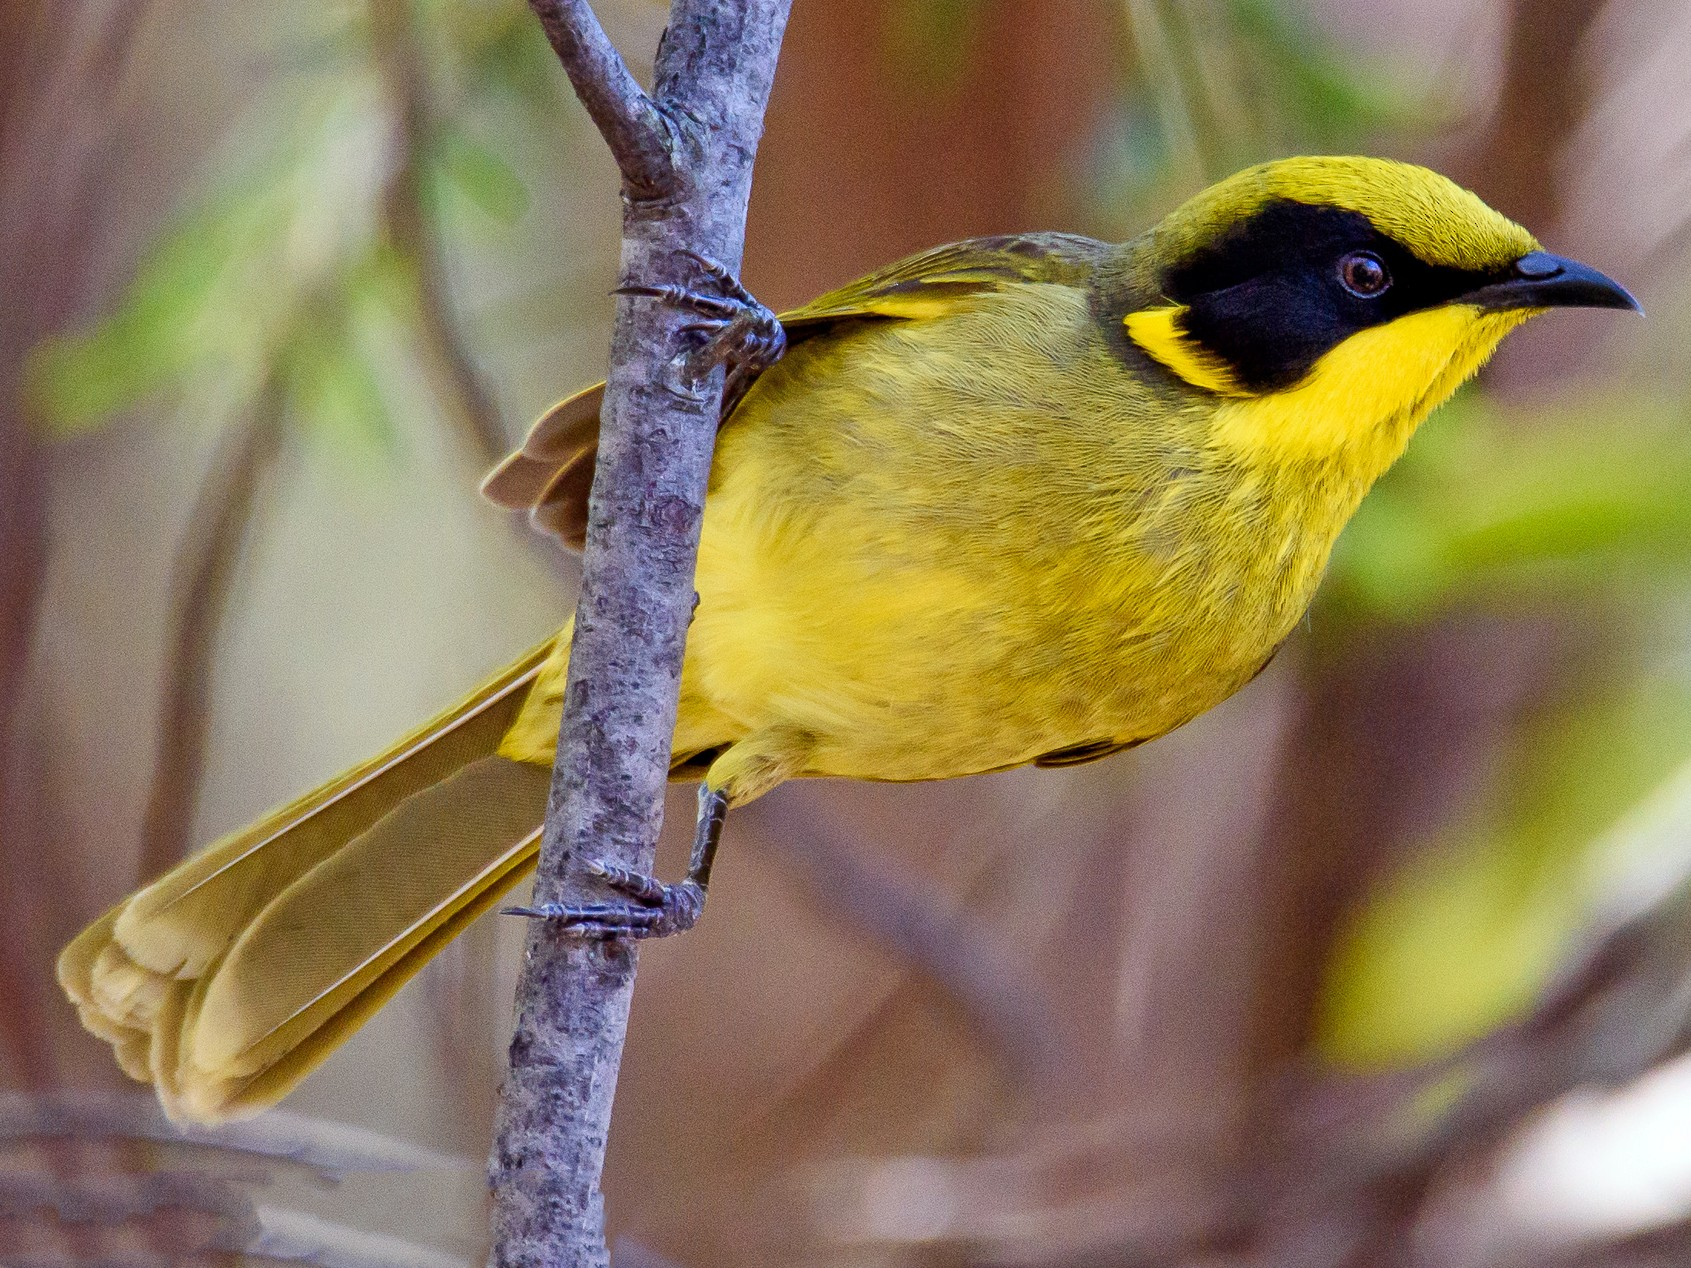
\includegraphics{images/Yellow_Tufted_Honeyeater.jpg}

}

\caption{The Yellow Tufted Honeyeater}

\end{figure}

\hypertarget{load-data}{%
\section*{Load data}\label{load-data}}
\addcontentsline{toc}{section}{Load data}

\markright{Load data}

\begin{Shaded}
\begin{Highlighting}[]
\FunctionTok{data}\NormalTok{(}\StringTok{"YTH"}\NormalTok{)}
\NormalTok{YTH  }\CommentTok{\# Explore the dataset}
\end{Highlighting}
\end{Shaded}

\begin{verbatim}
 ********************
 *** DARTR OBJECT ***
 ********************

 ** 609 genotypes,  994 SNPs , size: 49.9 Mb

    missing data: 139174 (=22.99 %) scored as NA

 ** Genetic data
   @gen: list of 609 SNPbin
   @ploidy: ploidy of each individual  (range: 2-2)

 ** Additional data
   @ind.names:  609 individual labels
   @loc.names:  994 locus labels
   @loc.all:  994 allele labels
   @position: integer storing positions of the SNPs [within 69 base sequence]
   @pop: population of each individual (group size range: 12-516)
   @other: a list containing: loc.metrics, ind.metrics, loc.metrics.flags, verbose, history 
    @other$ind.metrics: id, pop, sex, sex_original, service, plate_location 
    @other$loc.metrics: AlleleID, CloneID, AlleleSequence, TrimmedSequence, Chrom_Lichenostomus_HeHo_v1, ChromPos_Lichenostomus_HeHo_v1, AlnCnt_Lichenostomus_HeHo_v1, AlnEvalue_Lichenostomus_HeHo_v1, SNP, SnpPosition, CallRate, OneRatioRef, OneRatioSnp, FreqHomRef, FreqHomSnp, FreqHets, PICRef, PICSnp, AvgPIC, AvgCountRef, AvgCountSnp, RepAvg, clone, uid, rdepth, maf 
   @other$latlon[g]: no coordinates attached
\end{verbatim}

\begin{Shaded}
\begin{Highlighting}[]
\NormalTok{YTH}\SpecialCharTok{@}\NormalTok{n.loc  }\CommentTok{\# Number of SNPs}
\end{Highlighting}
\end{Shaded}

\begin{verbatim}
[1] 994
\end{verbatim}

\begin{Shaded}
\begin{Highlighting}[]
\FunctionTok{length}\NormalTok{(YTH}\SpecialCharTok{@}\NormalTok{ind.names)  }\CommentTok{\# Number of individuals}
\end{Highlighting}
\end{Shaded}

\begin{verbatim}
[1] 609
\end{verbatim}

\hypertarget{run-filter.sex.linked}{%
\section*{\texorpdfstring{Run
\texttt{filter.sex.linked}}{Run filter.sex.linked}}\label{run-filter.sex.linked}}
\addcontentsline{toc}{section}{Run \texttt{filter.sex.linked}}

\markright{Run \texttt{filter.sex.linked}}

This function identifies sex-linked and autosomal loci present in a SNP
dataset (i.e., genlight object) using individuals with known sex. It
identifies five types of loci: w-linked or y-linked, sex-biased,
z-linked or x-linked, gametologous and autosomal.

\emph{The genlight object must contain in gl@other\$ind.metrics a column
named ``id'', and a column named ``sex'' in which individuals with
known-sex are assigned `M' for male, or `F' for female. The function
ignores individuals that are assigned anything else or nothing at all
(unknown-sex).}

\begin{figure}

{\centering 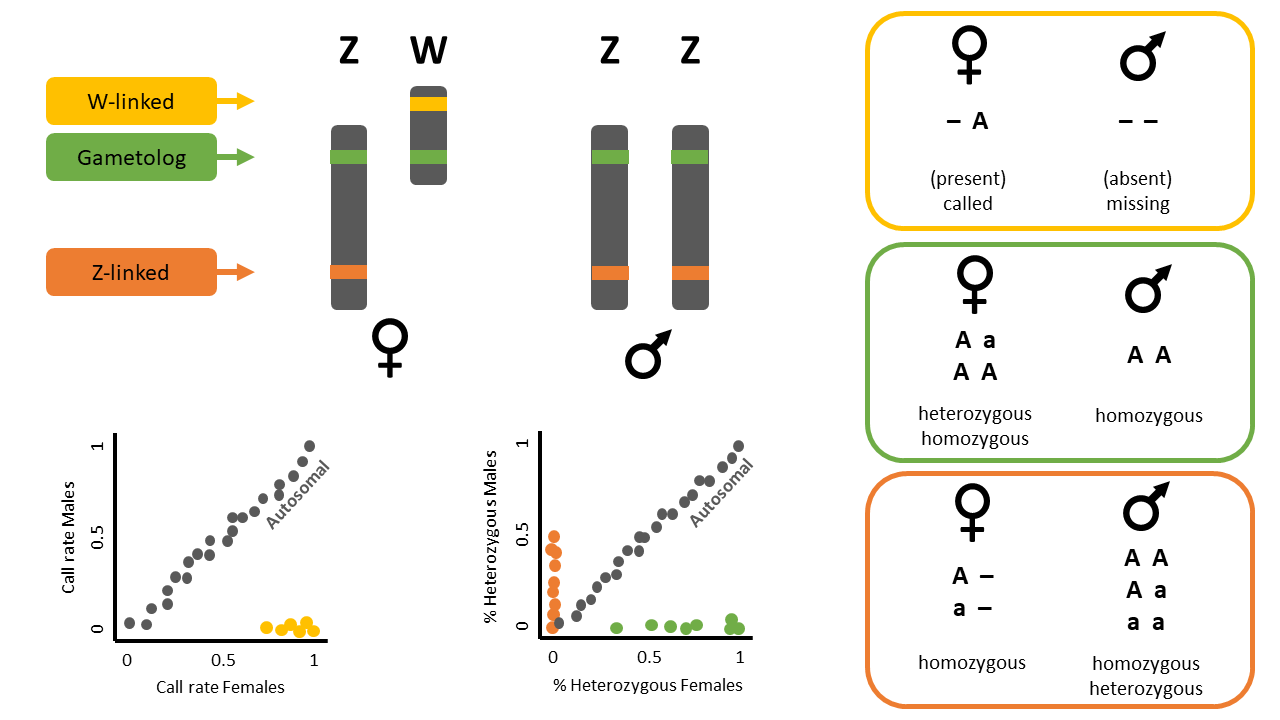
\includegraphics{images/ZW.png}

}

\caption{ZW/ZZ sex chromosomes}

\end{figure}

\textbf{NOTE}

Set \texttt{ncores} to more than 1 (default) if you have more than
50,000 SNPs, since it could actually slow down the analysis with smaller
datasets.

\begin{Shaded}
\begin{Highlighting}[]
\NormalTok{knitr}\SpecialCharTok{::}\FunctionTok{kable}\NormalTok{(}\FunctionTok{head}\NormalTok{(YTH}\SpecialCharTok{@}\NormalTok{other}\SpecialCharTok{$}\NormalTok{ind.metrics))  }\CommentTok{\# Check that ind.metrics has the necessary columns}
\end{Highlighting}
\end{Shaded}

\begin{longtable}[]{@{}
  >{\raggedright\arraybackslash}p{(\columnwidth - 12\tabcolsep) * \real{0.1351}}
  >{\raggedright\arraybackslash}p{(\columnwidth - 12\tabcolsep) * \real{0.1351}}
  >{\raggedright\arraybackslash}p{(\columnwidth - 12\tabcolsep) * \real{0.1216}}
  >{\raggedright\arraybackslash}p{(\columnwidth - 12\tabcolsep) * \real{0.0541}}
  >{\raggedright\arraybackslash}p{(\columnwidth - 12\tabcolsep) * \real{0.1757}}
  >{\raggedright\arraybackslash}p{(\columnwidth - 12\tabcolsep) * \real{0.1757}}
  >{\raggedright\arraybackslash}p{(\columnwidth - 12\tabcolsep) * \real{0.2027}}@{}}
\toprule\noalign{}
\begin{minipage}[b]{\linewidth}\raggedright
\end{minipage} & \begin{minipage}[b]{\linewidth}\raggedright
id
\end{minipage} & \begin{minipage}[b]{\linewidth}\raggedright
pop
\end{minipage} & \begin{minipage}[b]{\linewidth}\raggedright
sex
\end{minipage} & \begin{minipage}[b]{\linewidth}\raggedright
sex\_original
\end{minipage} & \begin{minipage}[b]{\linewidth}\raggedright
service
\end{minipage} & \begin{minipage}[b]{\linewidth}\raggedright
plate\_location
\end{minipage} \\
\midrule\noalign{}
\endhead
\bottomrule\noalign{}
\endlastfoot
ANWC46839 & ANWC46839 & Melanops & F & F & DLich17-2918 & 1-A1 \\
W49 & W49 & Cassidix & F & F & DLich17-2918 & 1-A10 \\
W90 & W90 & Cassidix & F & F & DLich17-2918 & 1-A12 \\
C25 & C25 & Cassidix & M & M & DLich17-2918 & 1-A2 \\
C8 & C8 & Cassidix & M & M & DLich17-2918 & 1-A3 \\
W70 & W70 & Cassidix & F & F & DLich17-2918 & 1-A4 \\
\end{longtable}

\begin{Shaded}
\begin{Highlighting}[]
\NormalTok{res }\OtherTok{\textless{}{-}}\NormalTok{ dartR.sexlinked}\SpecialCharTok{::}\FunctionTok{filter.sex.linked}\NormalTok{(}\AttributeTok{gl =}\NormalTok{ YTH, }\AttributeTok{system =} \StringTok{"zw"}\NormalTok{)}
\end{Highlighting}
\end{Shaded}

\begin{verbatim}
Detected 276 females and 333 males.
\end{verbatim}

\begin{verbatim}
Starting phase 1. May take a while...
\end{verbatim}

\begin{verbatim}
Building call rate plots.
\end{verbatim}

\begin{figure}[H]

{\centering \includegraphics{Session10_SexLinkedMarkers_files/figure-pdf/unnamed-chunk-3-1.pdf}

}

\end{figure}

\begin{verbatim}
Done. Starting phase 2.
\end{verbatim}

\begin{verbatim}
Building heterozygosity plots.
\end{verbatim}

\begin{figure}[H]

{\centering 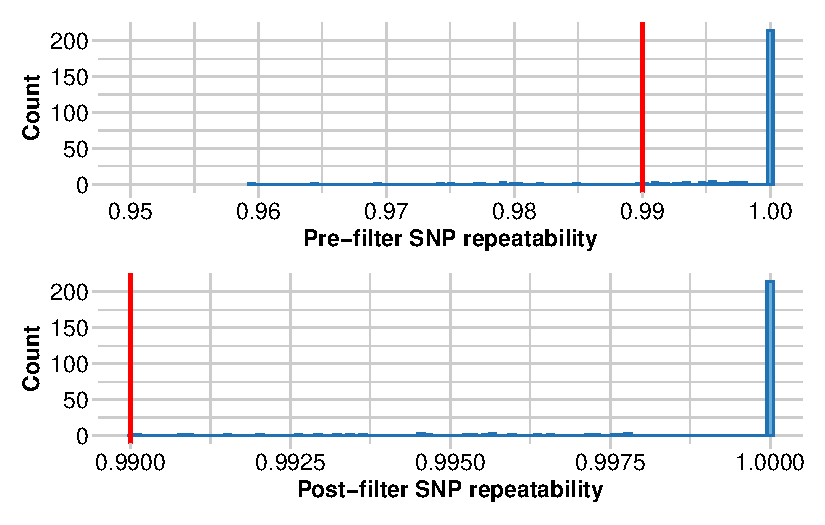
\includegraphics{Session10_SexLinkedMarkers_files/figure-pdf/unnamed-chunk-3-2.pdf}

}

\end{figure}

\begin{figure}[H]

{\centering 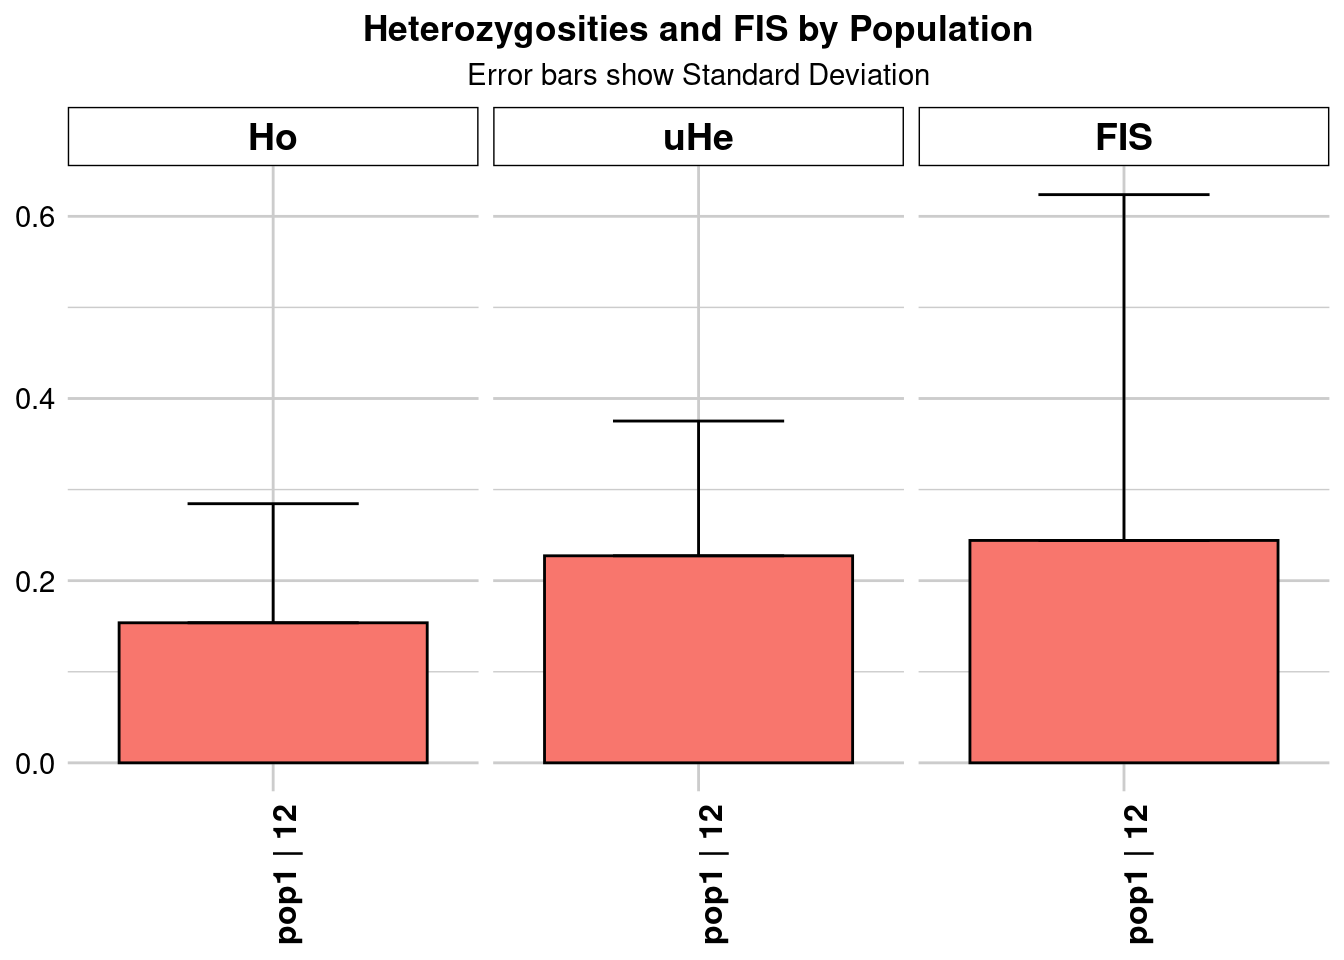
\includegraphics{Session10_SexLinkedMarkers_files/figure-pdf/unnamed-chunk-3-3.pdf}

}

\end{figure}

\begin{verbatim}
Done building heterozygosity plots.
\end{verbatim}

\begin{verbatim}
**FINISHED** Total of analyzed loci: 994.
Found 506 sex-linked loci:
   52 W-linked loci
   273 sex-biased loci
   165 Z-linked loci
   16 ZW gametologs.
And 488 autosomal loci.
\end{verbatim}

\begin{figure}[H]

{\centering 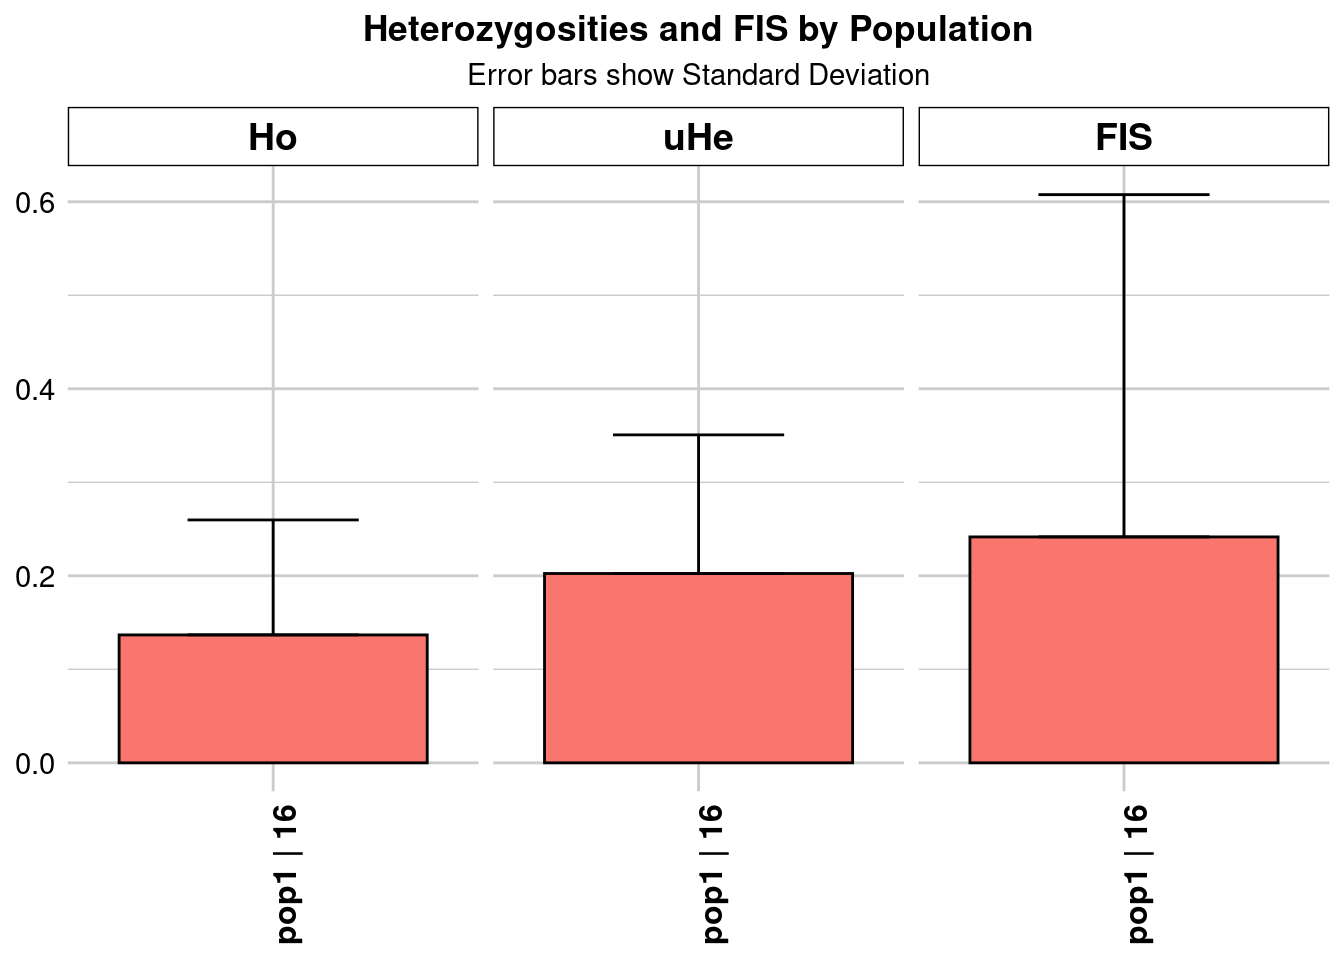
\includegraphics{Session10_SexLinkedMarkers_files/figure-pdf/unnamed-chunk-3-4.pdf}

}

\end{figure}

\begin{tcolorbox}[enhanced jigsaw, coltitle=black, colframe=quarto-callout-note-color-frame, colbacktitle=quarto-callout-note-color!10!white, breakable, bottomtitle=1mm, rightrule=.15mm, opacitybacktitle=0.6, left=2mm, arc=.35mm, opacityback=0, leftrule=.75mm, toptitle=1mm, titlerule=0mm, title=\textcolor{quarto-callout-note-color}{\faInfo}\hspace{0.5em}{Exercise}, bottomrule=.15mm, toprule=.15mm, colback=white]


\includegraphics[width=0.5in,height=0.5in]{images/task.png}

How many males and females does the dataset contain?

How many sex-linked loci were found?

\end{tcolorbox}

Now check the output:

\begin{Shaded}
\begin{Highlighting}[]
\NormalTok{res}\SpecialCharTok{$}\NormalTok{w.linked  }\CommentTok{\# Notice that it says \textquotesingle{}w{-}linked\textquotesingle{}}
\end{Highlighting}
\end{Shaded}

\begin{verbatim}
 ********************
 *** DARTR OBJECT ***
 ********************

 ** 609 genotypes,  52 SNPs , size: 48.9 Mb

    missing data: 17304 (=54.64 %) scored as NA

 ** Genetic data
   @gen: list of 609 SNPbin
   @ploidy: ploidy of each individual  (range: 2-2)

 ** Additional data
   @ind.names:  609 individual labels
   @loc.names:  52 locus labels
   @loc.all:  52 allele labels
   @position: integer storing positions of the SNPs [within 69 base sequence]
   @pop: population of each individual (group size range: 12-516)
   @other: a list containing: loc.metrics, ind.metrics, loc.metrics.flags, verbose, history 
    @other$ind.metrics: id, pop, sex, sex_original, service, plate_location 
    @other$loc.metrics: AlleleID, CloneID, AlleleSequence, TrimmedSequence, Chrom_Lichenostomus_HeHo_v1, ChromPos_Lichenostomus_HeHo_v1, AlnCnt_Lichenostomus_HeHo_v1, AlnEvalue_Lichenostomus_HeHo_v1, SNP, SnpPosition, CallRate, OneRatioRef, OneRatioSnp, FreqHomRef, FreqHomSnp, FreqHets, PICRef, PICSnp, AvgPIC, AvgCountRef, AvgCountSnp, RepAvg, clone, uid, rdepth, maf 
   @other$latlon[g]: no coordinates attached
\end{verbatim}

\begin{Shaded}
\begin{Highlighting}[]
\NormalTok{res}\SpecialCharTok{$}\NormalTok{z.linked  }\CommentTok{\# Notice that it says \textquotesingle{}z{-}linked\textquotesingle{}}
\end{Highlighting}
\end{Shaded}

\begin{verbatim}
 ********************
 *** DARTR OBJECT ***
 ********************

 ** 609 genotypes,  165 SNPs , size: 48.9 Mb

    missing data: 2990 (=2.98 %) scored as NA

 ** Genetic data
   @gen: list of 609 SNPbin
   @ploidy: ploidy of each individual  (range: 2-2)

 ** Additional data
   @ind.names:  609 individual labels
   @loc.names:  165 locus labels
   @loc.all:  165 allele labels
   @position: integer storing positions of the SNPs [within 69 base sequence]
   @pop: population of each individual (group size range: 12-516)
   @other: a list containing: loc.metrics, ind.metrics, loc.metrics.flags, verbose, history 
    @other$ind.metrics: id, pop, sex, sex_original, service, plate_location 
    @other$loc.metrics: AlleleID, CloneID, AlleleSequence, TrimmedSequence, Chrom_Lichenostomus_HeHo_v1, ChromPos_Lichenostomus_HeHo_v1, AlnCnt_Lichenostomus_HeHo_v1, AlnEvalue_Lichenostomus_HeHo_v1, SNP, SnpPosition, CallRate, OneRatioRef, OneRatioSnp, FreqHomRef, FreqHomSnp, FreqHets, PICRef, PICSnp, AvgPIC, AvgCountRef, AvgCountSnp, RepAvg, clone, uid, rdepth, maf 
   @other$latlon[g]: no coordinates attached
\end{verbatim}

\begin{Shaded}
\begin{Highlighting}[]
\NormalTok{res}\SpecialCharTok{$}\NormalTok{gametolog}
\end{Highlighting}
\end{Shaded}

\begin{verbatim}
 ********************
 *** DARTR OBJECT ***
 ********************

 ** 609 genotypes,  16 SNPs , size: 48.8 Mb

    missing data: 580 (=5.95 %) scored as NA

 ** Genetic data
   @gen: list of 609 SNPbin
   @ploidy: ploidy of each individual  (range: 2-2)

 ** Additional data
   @ind.names:  609 individual labels
   @loc.names:  16 locus labels
   @loc.all:  16 allele labels
   @position: integer storing positions of the SNPs [within 69 base sequence]
   @pop: population of each individual (group size range: 12-516)
   @other: a list containing: loc.metrics, ind.metrics, loc.metrics.flags, verbose, history 
    @other$ind.metrics: id, pop, sex, sex_original, service, plate_location 
    @other$loc.metrics: AlleleID, CloneID, AlleleSequence, TrimmedSequence, Chrom_Lichenostomus_HeHo_v1, ChromPos_Lichenostomus_HeHo_v1, AlnCnt_Lichenostomus_HeHo_v1, AlnEvalue_Lichenostomus_HeHo_v1, SNP, SnpPosition, CallRate, OneRatioRef, OneRatioSnp, FreqHomRef, FreqHomSnp, FreqHets, PICRef, PICSnp, AvgPIC, AvgCountRef, AvgCountSnp, RepAvg, clone, uid, rdepth, maf 
   @other$latlon[g]: no coordinates attached
\end{verbatim}

\begin{Shaded}
\begin{Highlighting}[]
\NormalTok{res}\SpecialCharTok{$}\NormalTok{sex.biased}
\end{Highlighting}
\end{Shaded}

\begin{verbatim}
 ********************
 *** DARTR OBJECT ***
 ********************

 ** 609 genotypes,  273 SNPs , size: 49.2 Mb

    missing data: 46048 (=27.7 %) scored as NA

 ** Genetic data
   @gen: list of 609 SNPbin
   @ploidy: ploidy of each individual  (range: 2-2)

 ** Additional data
   @ind.names:  609 individual labels
   @loc.names:  273 locus labels
   @loc.all:  273 allele labels
   @position: integer storing positions of the SNPs [within 69 base sequence]
   @pop: population of each individual (group size range: 12-516)
   @other: a list containing: loc.metrics, ind.metrics, loc.metrics.flags, verbose, history 
    @other$ind.metrics: id, pop, sex, sex_original, service, plate_location 
    @other$loc.metrics: AlleleID, CloneID, AlleleSequence, TrimmedSequence, Chrom_Lichenostomus_HeHo_v1, ChromPos_Lichenostomus_HeHo_v1, AlnCnt_Lichenostomus_HeHo_v1, AlnEvalue_Lichenostomus_HeHo_v1, SNP, SnpPosition, CallRate, OneRatioRef, OneRatioSnp, FreqHomRef, FreqHomSnp, FreqHets, PICRef, PICSnp, AvgPIC, AvgCountRef, AvgCountSnp, RepAvg, clone, uid, rdepth, maf 
   @other$latlon[g]: no coordinates attached
\end{verbatim}

\begin{Shaded}
\begin{Highlighting}[]
\NormalTok{res}\SpecialCharTok{$}\NormalTok{autosomal}
\end{Highlighting}
\end{Shaded}

\begin{verbatim}
 ********************
 *** DARTR OBJECT ***
 ********************

 ** 609 genotypes,  488 SNPs , size: 49.4 Mb

    missing data: 72252 (=24.31 %) scored as NA

 ** Genetic data
   @gen: list of 609 SNPbin
   @ploidy: ploidy of each individual  (range: 2-2)

 ** Additional data
   @ind.names:  609 individual labels
   @loc.names:  488 locus labels
   @loc.all:  488 allele labels
   @position: integer storing positions of the SNPs [within 69 base sequence]
   @pop: population of each individual (group size range: 12-516)
   @other: a list containing: loc.metrics, ind.metrics, loc.metrics.flags, verbose, history 
    @other$ind.metrics: id, pop, sex, sex_original, service, plate_location 
    @other$loc.metrics: AlleleID, CloneID, AlleleSequence, TrimmedSequence, Chrom_Lichenostomus_HeHo_v1, ChromPos_Lichenostomus_HeHo_v1, AlnCnt_Lichenostomus_HeHo_v1, AlnEvalue_Lichenostomus_HeHo_v1, SNP, SnpPosition, CallRate, OneRatioRef, OneRatioSnp, FreqHomRef, FreqHomSnp, FreqHets, PICRef, PICSnp, AvgPIC, AvgCountRef, AvgCountSnp, RepAvg, clone, uid, rdepth, maf 
   @other$latlon[g]: no coordinates attached
\end{verbatim}

\begin{Shaded}
\begin{Highlighting}[]
\NormalTok{knitr}\SpecialCharTok{::}\FunctionTok{kable}\NormalTok{(}\FunctionTok{head}\NormalTok{(res}\SpecialCharTok{$}\NormalTok{results.table))  }\CommentTok{\# The output table}
\end{Highlighting}
\end{Shaded}

\begin{longtable}[]{@{}
  >{\raggedright\arraybackslash}p{(\columnwidth - 46\tabcolsep) * \real{0.0533}}
  >{\raggedleft\arraybackslash}p{(\columnwidth - 46\tabcolsep) * \real{0.0200}}
  >{\raggedleft\arraybackslash}p{(\columnwidth - 46\tabcolsep) * \real{0.0433}}
  >{\raggedleft\arraybackslash}p{(\columnwidth - 46\tabcolsep) * \real{0.0433}}
  >{\raggedleft\arraybackslash}p{(\columnwidth - 46\tabcolsep) * \real{0.0500}}
  >{\raggedleft\arraybackslash}p{(\columnwidth - 46\tabcolsep) * \real{0.0500}}
  >{\raggedleft\arraybackslash}p{(\columnwidth - 46\tabcolsep) * \real{0.0333}}
  >{\raggedleft\arraybackslash}p{(\columnwidth - 46\tabcolsep) * \real{0.0333}}
  >{\raggedleft\arraybackslash}p{(\columnwidth - 46\tabcolsep) * \real{0.0367}}
  >{\raggedleft\arraybackslash}p{(\columnwidth - 46\tabcolsep) * \real{0.0467}}
  >{\raggedleft\arraybackslash}p{(\columnwidth - 46\tabcolsep) * \real{0.0467}}
  >{\raggedright\arraybackslash}p{(\columnwidth - 46\tabcolsep) * \real{0.0300}}
  >{\raggedright\arraybackslash}p{(\columnwidth - 46\tabcolsep) * \real{0.0367}}
  >{\raggedleft\arraybackslash}p{(\columnwidth - 46\tabcolsep) * \real{0.0400}}
  >{\raggedleft\arraybackslash}p{(\columnwidth - 46\tabcolsep) * \real{0.0400}}
  >{\raggedleft\arraybackslash}p{(\columnwidth - 46\tabcolsep) * \real{0.0400}}
  >{\raggedleft\arraybackslash}p{(\columnwidth - 46\tabcolsep) * \real{0.0400}}
  >{\raggedleft\arraybackslash}p{(\columnwidth - 46\tabcolsep) * \real{0.0333}}
  >{\raggedleft\arraybackslash}p{(\columnwidth - 46\tabcolsep) * \real{0.0433}}
  >{\raggedleft\arraybackslash}p{(\columnwidth - 46\tabcolsep) * \real{0.0533}}
  >{\raggedleft\arraybackslash}p{(\columnwidth - 46\tabcolsep) * \real{0.0567}}
  >{\raggedleft\arraybackslash}p{(\columnwidth - 46\tabcolsep) * \real{0.0567}}
  >{\raggedright\arraybackslash}p{(\columnwidth - 46\tabcolsep) * \real{0.0300}}
  >{\raggedright\arraybackslash}p{(\columnwidth - 46\tabcolsep) * \real{0.0433}}@{}}
\toprule\noalign{}
\begin{minipage}[b]{\linewidth}\raggedright
\end{minipage} & \begin{minipage}[b]{\linewidth}\raggedleft
index
\end{minipage} & \begin{minipage}[b]{\linewidth}\raggedleft
count.F.miss
\end{minipage} & \begin{minipage}[b]{\linewidth}\raggedleft
count.M.miss
\end{minipage} & \begin{minipage}[b]{\linewidth}\raggedleft
count.F.scored
\end{minipage} & \begin{minipage}[b]{\linewidth}\raggedleft
count.M.scored
\end{minipage} & \begin{minipage}[b]{\linewidth}\raggedleft
ratio
\end{minipage} & \begin{minipage}[b]{\linewidth}\raggedleft
p.value
\end{minipage} & \begin{minipage}[b]{\linewidth}\raggedleft
p.adjusted
\end{minipage} & \begin{minipage}[b]{\linewidth}\raggedleft
scoringRate.F
\end{minipage} & \begin{minipage}[b]{\linewidth}\raggedleft
scoringRate.M
\end{minipage} & \begin{minipage}[b]{\linewidth}\raggedright
w.linked
\end{minipage} & \begin{minipage}[b]{\linewidth}\raggedright
sex.biased
\end{minipage} & \begin{minipage}[b]{\linewidth}\raggedleft
count.F.het
\end{minipage} & \begin{minipage}[b]{\linewidth}\raggedleft
count.M.het
\end{minipage} & \begin{minipage}[b]{\linewidth}\raggedleft
count.F.hom
\end{minipage} & \begin{minipage}[b]{\linewidth}\raggedleft
count.M.hom
\end{minipage} & \begin{minipage}[b]{\linewidth}\raggedleft
stat
\end{minipage} & \begin{minipage}[b]{\linewidth}\raggedleft
stat.p.value
\end{minipage} & \begin{minipage}[b]{\linewidth}\raggedleft
stat.p.adjusted
\end{minipage} & \begin{minipage}[b]{\linewidth}\raggedleft
heterozygosity.F
\end{minipage} & \begin{minipage}[b]{\linewidth}\raggedleft
heterozygosity.M
\end{minipage} & \begin{minipage}[b]{\linewidth}\raggedright
z.linked
\end{minipage} & \begin{minipage}[b]{\linewidth}\raggedright
zw.gametolog
\end{minipage} \\
\midrule\noalign{}
\endhead
\bottomrule\noalign{}
\endlastfoot
27382025-26-T/C & 1 & 61 & 25 & 215 & 308 & 3.4882302 & 0.0000003 &
0.0000016 & 0.7789855 & 0.9249249 & FALSE & TRUE & 0 & 73 & 215 & 235 &
NA & NA & NA & 0.0000000 & 0.2370130 & FALSE & FALSE \\
27338005-34-A/G & 2 & 12 & 13 & 264 & 320 & 1.1186728 & 0.8390268 &
1.0000000 & 0.9565217 & 0.9609610 & FALSE & FALSE & 0 & 144 & 264 & 176
& 0.0046581 & 0.0000000 & 0.0000000 & 0.0000000 & 0.4500000 & TRUE &
FALSE \\
27331627-16-T/G & 3 & 108 & 159 & 168 & 174 & 0.7039235 & 0.0334301 &
0.0860868 & 0.6086957 & 0.5225225 & FALSE & FALSE & 0 & 2 & 168 & 172 &
0.5128690 & 1.0000000 & 1.0000000 & 0.0000000 & 0.0114943 & FALSE &
FALSE \\
53948461-35-G/A & 4 & 46 & 64 & 230 & 269 & 0.8408645 & 0.4593502 &
0.7791707 & 0.8333333 & 0.8078078 & FALSE & FALSE & 29 & 27 & 201 & 242
& 1.2924846 & 0.3950852 & 0.9051780 & 0.1260870 & 0.1003717 & FALSE &
FALSE \\
27360874-8-A/G & 5 & 41 & 63 & 235 & 270 & 0.7480768 & 0.1956613 &
0.4120495 & 0.8514493 & 0.8108108 & FALSE & FALSE & 25 & 38 & 210 & 232
& 0.7272744 & 0.2807852 & 0.7009152 & 0.1063830 & 0.1407407 & FALSE &
FALSE \\
27377678-32-C/A & 6 & 30 & 33 & 246 & 300 & 1.1084581 & 0.7894511 &
1.0000000 & 0.8913043 & 0.9009009 & FALSE & FALSE & 3 & 6 & 243 & 294 &
0.6054740 & 0.5234966 & 1.0000000 & 0.0121951 & 0.0200000 & FALSE &
FALSE \\
\end{longtable}

The output consists of a genlight object for each type of loci, plus a
results table.

\hypertarget{run-infer.sex}{%
\section*{\texorpdfstring{Run
\texttt{infer.sex}}{Run infer.sex}}\label{run-infer.sex}}
\addcontentsline{toc}{section}{Run \texttt{infer.sex}}

\markright{Run \texttt{infer.sex}}

This function uses the complete output of function filter.sex.linked
(list of 6 objects) to infer the sex of all individuals in the dataset.
Specifically, the function uses 3 types of sex-linked loci (W-/Y-linked,
Z-/X-linked, and gametologs), assigns a preliminary genetic sex for each
type of sex-linked loci available, and outputs an \texttt{agreed\ sex}.

\begin{Shaded}
\begin{Highlighting}[]
\NormalTok{sexID }\OtherTok{\textless{}{-}}\NormalTok{ dartR.sexlinked}\SpecialCharTok{::}\FunctionTok{infer.sex}\NormalTok{(}\AttributeTok{gl\_sex\_filtered =}\NormalTok{ res, }\AttributeTok{system =} \StringTok{"zw"}\NormalTok{,}
    \AttributeTok{seed =} \DecValTok{124}\NormalTok{)}
\end{Highlighting}
\end{Shaded}

\begin{verbatim}
***FINISHED***
\end{verbatim}

\begin{Shaded}
\begin{Highlighting}[]
\NormalTok{knitr}\SpecialCharTok{::}\FunctionTok{kable}\NormalTok{(}\FunctionTok{head}\NormalTok{(sexID))}
\end{Highlighting}
\end{Shaded}

\begin{longtable}[]{@{}
  >{\raggedright\arraybackslash}p{(\columnwidth - 22\tabcolsep) * \real{0.0862}}
  >{\raggedright\arraybackslash}p{(\columnwidth - 22\tabcolsep) * \real{0.0862}}
  >{\raggedright\arraybackslash}p{(\columnwidth - 22\tabcolsep) * \real{0.1121}}
  >{\raggedleft\arraybackslash}p{(\columnwidth - 22\tabcolsep) * \real{0.0776}}
  >{\raggedleft\arraybackslash}p{(\columnwidth - 22\tabcolsep) * \real{0.0690}}
  >{\raggedright\arraybackslash}p{(\columnwidth - 22\tabcolsep) * \real{0.1121}}
  >{\raggedleft\arraybackslash}p{(\columnwidth - 22\tabcolsep) * \real{0.0603}}
  >{\raggedleft\arraybackslash}p{(\columnwidth - 22\tabcolsep) * \real{0.0603}}
  >{\raggedright\arraybackslash}p{(\columnwidth - 22\tabcolsep) * \real{0.1207}}
  >{\raggedleft\arraybackslash}p{(\columnwidth - 22\tabcolsep) * \real{0.0603}}
  >{\raggedleft\arraybackslash}p{(\columnwidth - 22\tabcolsep) * \real{0.0603}}
  >{\raggedright\arraybackslash}p{(\columnwidth - 22\tabcolsep) * \real{0.0948}}@{}}
\toprule\noalign{}
\begin{minipage}[b]{\linewidth}\raggedright
\end{minipage} & \begin{minipage}[b]{\linewidth}\raggedright
id
\end{minipage} & \begin{minipage}[b]{\linewidth}\raggedright
w.linked.sex
\end{minipage} & \begin{minipage}[b]{\linewidth}\raggedleft
\#missing
\end{minipage} & \begin{minipage}[b]{\linewidth}\raggedleft
\#called
\end{minipage} & \begin{minipage}[b]{\linewidth}\raggedright
z.linked.sex
\end{minipage} & \begin{minipage}[b]{\linewidth}\raggedleft
\#Hom.z
\end{minipage} & \begin{minipage}[b]{\linewidth}\raggedleft
\#Het.z
\end{minipage} & \begin{minipage}[b]{\linewidth}\raggedright
gametolog.sex
\end{minipage} & \begin{minipage}[b]{\linewidth}\raggedleft
\#Hom.g
\end{minipage} & \begin{minipage}[b]{\linewidth}\raggedleft
\#Het.g
\end{minipage} & \begin{minipage}[b]{\linewidth}\raggedright
agreed.sex
\end{minipage} \\
\midrule\noalign{}
\endhead
\bottomrule\noalign{}
\endlastfoot
ANWC46839 & ANWC46839 & F & 51 & 1 & F & 1 & 141 & F & 5 & 0 & F \\
W49 & W49 & F & 52 & 0 & F & 2 & 156 & F & 5 & 0 & F \\
W90 & W90 & F & 48 & 4 & F & 0 & 162 & F & 5 & 0 & F \\
C25 & C25 & M & 0 & 52 & M & 52 & 113 & M & 0 & 5 & M \\
C8 & C8 & M & 0 & 52 & M & 48 & 116 & M & 0 & 5 & M \\
W70 & W70 & F & 49 & 3 & F & 0 & 152 & F & 5 & 0 & F \\
\end{longtable}

\begin{tcolorbox}[enhanced jigsaw, coltitle=black, colframe=quarto-callout-warning-color-frame, colbacktitle=quarto-callout-warning-color!10!white, breakable, bottomtitle=1mm, rightrule=.15mm, opacitybacktitle=0.6, left=2mm, arc=.35mm, opacityback=0, leftrule=.75mm, toptitle=1mm, titlerule=0mm, title=\textcolor{quarto-callout-warning-color}{\faExclamationTriangle}\hspace{0.5em}{Warning}, bottomrule=.15mm, toprule=.15mm, colback=white]

\textbf{IMPORTANT} We created this function with the explicit intent
that a human checks the evidence for the \texttt{agreed\ sex} that do
NOT agree for all types of sex-linked loci (denoted as `*M' or `*F').
This human can then use their criterion to validate these assignments.

\end{tcolorbox}

\begin{tcolorbox}[enhanced jigsaw, coltitle=black, colframe=quarto-callout-note-color-frame, colbacktitle=quarto-callout-note-color!10!white, breakable, bottomtitle=1mm, rightrule=.15mm, opacitybacktitle=0.6, left=2mm, arc=.35mm, opacityback=0, leftrule=.75mm, toptitle=1mm, titlerule=0mm, title=\textcolor{quarto-callout-note-color}{\faInfo}\hspace{0.5em}{Exercise}, bottomrule=.15mm, toprule=.15mm, colback=white]


\includegraphics[width=0.5in,height=0.5in]{images/task.png}

Can you find individuals for which the \texttt{agreed\ sex} is uncertain
(i.e., has an asterisk ``*'')?

\end{tcolorbox}

\bookmarksetup{startatroot}

\hypertarget{dataset-2---xxxy---the-leadbeaters-possum}{%
\chapter*{Dataset 2 - XX/XY - The Leadbeater's
possum}\label{dataset-2---xxxy---the-leadbeaters-possum}}
\addcontentsline{toc}{chapter}{Dataset 2 - XX/XY - The Leadbeater's
possum}

\markboth{Dataset 2 - XX/XY - The Leadbeater's possum}{Dataset 2 - XX/XY
- The Leadbeater's possum}

\begin{figure}

{\centering 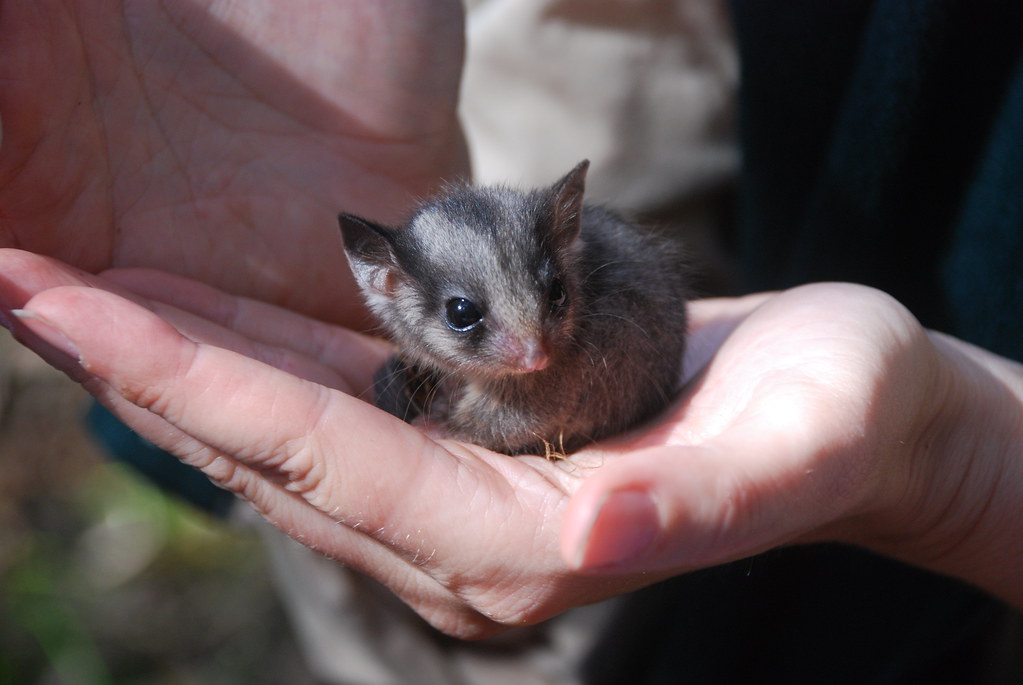
\includegraphics{images/Leadbeaters_possum.jpg}

}

\caption{The Leadbeater's possum}

\end{figure}

\hypertarget{load-data-1}{%
\section*{Load data}\label{load-data-1}}
\addcontentsline{toc}{section}{Load data}

\markright{Load data}

\begin{Shaded}
\begin{Highlighting}[]
\FunctionTok{data}\NormalTok{(}\StringTok{"LBP"}\NormalTok{)}
\NormalTok{LBP  }\CommentTok{\# Explore the dataset}
\end{Highlighting}
\end{Shaded}

\begin{verbatim}
 ********************
 *** DARTR OBJECT ***
 ********************

 ** 376 genotypes,  1,000 SNPs , size: 5.2 Mb

    missing data: 20670 (=5.5 %) scored as NA

 ** Genetic data
   @gen: list of 376 SNPbin
   @ploidy: ploidy of each individual  (range: 2-2)

 ** Additional data
   @ind.names:  376 individual labels
   @loc.names:  1000 locus labels
   @loc.all:  1000 allele labels
   @position: integer storing positions of the SNPs [within 69 base sequence]
   @pop: population of each individual (group size range: 95-281)
   @other: a list containing: loc.metrics, ind.metrics, loc.metrics.flags, verbose, history 
    @other$ind.metrics: id, sex, pop, Year.collected, service, plate_location 
    @other$loc.metrics: AlleleID, CloneID, AlleleSequence, TrimmedSequence, Chrom_Possum_v2, ChromPos_Possum_v2, AlnCnt_Possum_v2, AlnEvalue_Possum_v2, SNP, SnpPosition, CallRate, OneRatioRef, OneRatioSnp, FreqHomRef, FreqHomSnp, FreqHets, PICRef, PICSnp, AvgPIC, AvgCountRef, AvgCountSnp, RepAvg, clone, uid, rdepth, monomorphs, maf, OneRatio, PIC 
   @other$latlon[g]: no coordinates attached
\end{verbatim}

\begin{Shaded}
\begin{Highlighting}[]
\NormalTok{LBP}\SpecialCharTok{@}\NormalTok{n.loc  }\CommentTok{\# Number of SNPs}
\end{Highlighting}
\end{Shaded}

\begin{verbatim}
[1] 1000
\end{verbatim}

\begin{Shaded}
\begin{Highlighting}[]
\FunctionTok{length}\NormalTok{(LBP}\SpecialCharTok{@}\NormalTok{ind.names)  }\CommentTok{\# Number of individuals}
\end{Highlighting}
\end{Shaded}

\begin{verbatim}
[1] 376
\end{verbatim}

\hypertarget{run-filter.sex.linked-1}{%
\section*{\texorpdfstring{Run
\texttt{filter.sex.linked}}{Run filter.sex.linked}}\label{run-filter.sex.linked-1}}
\addcontentsline{toc}{section}{Run \texttt{filter.sex.linked}}

\markright{Run \texttt{filter.sex.linked}}

This function identifies sex-linked and autosomal loci present in a SNP
dataset (genlight object) using individuals with known sex. It
identifies five types of loci: w-linked or y-linked, sex-biased,
z-linked or x-linked, gametologous and autosomal.

\emph{The genlight object must contain in gl@other\$ind.metrics a column
named ``id'', and a column named ``sex'' in which individuals with
known-sex are assigned `M' for male, or `F' for female. The function
ignores individuals that are assigned anything else or nothing at all
(unknown-sex).}

\begin{figure}

{\centering 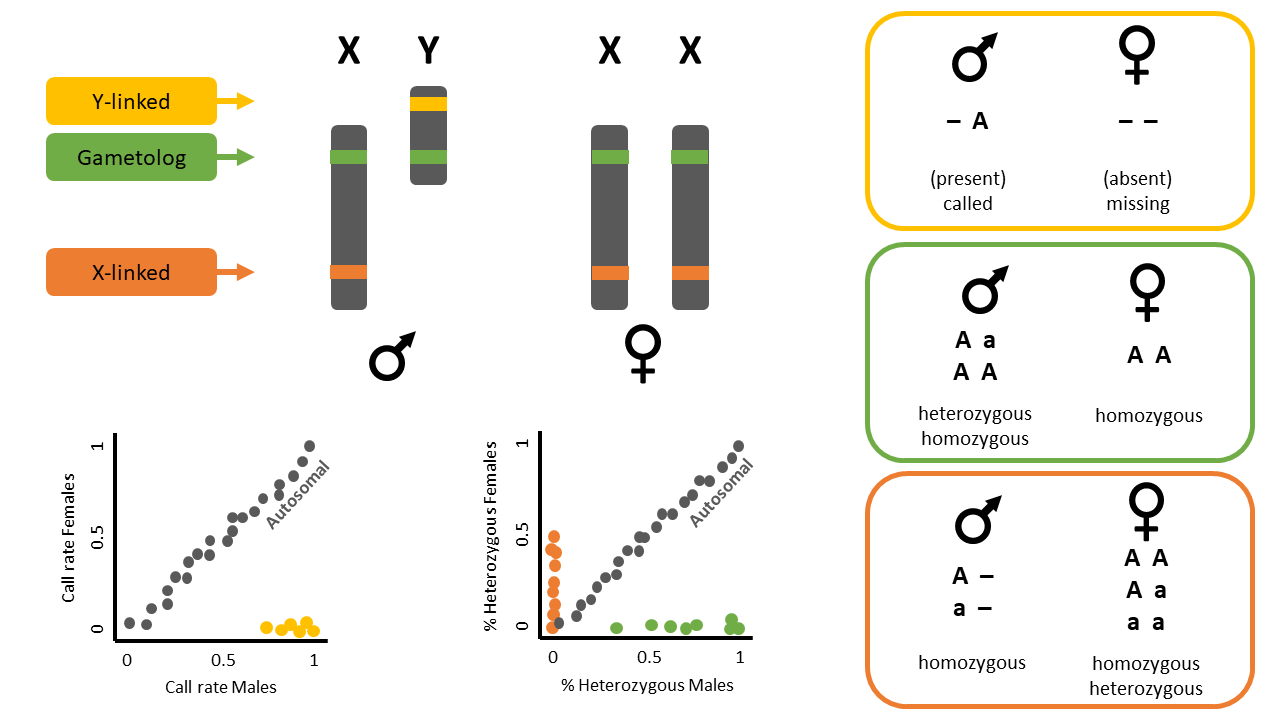
\includegraphics{images/XY.png}

}

\caption{XX/XY sex chromosomes}

\end{figure}

\begin{Shaded}
\begin{Highlighting}[]
\NormalTok{knitr}\SpecialCharTok{::}\FunctionTok{kable}\NormalTok{(}\FunctionTok{head}\NormalTok{(LBP}\SpecialCharTok{@}\NormalTok{other}\SpecialCharTok{$}\NormalTok{ind.metrics))  }\CommentTok{\# Check that ind.metrics has the necessary columns}
\end{Highlighting}
\end{Shaded}

\begin{longtable}[]{@{}
  >{\raggedright\arraybackslash}p{(\columnwidth - 12\tabcolsep) * \real{0.0615}}
  >{\raggedright\arraybackslash}p{(\columnwidth - 12\tabcolsep) * \real{0.0615}}
  >{\raggedright\arraybackslash}p{(\columnwidth - 12\tabcolsep) * \real{0.0615}}
  >{\raggedright\arraybackslash}p{(\columnwidth - 12\tabcolsep) * \real{0.1538}}
  >{\raggedleft\arraybackslash}p{(\columnwidth - 12\tabcolsep) * \real{0.2308}}
  >{\raggedright\arraybackslash}p{(\columnwidth - 12\tabcolsep) * \real{0.2000}}
  >{\raggedright\arraybackslash}p{(\columnwidth - 12\tabcolsep) * \real{0.2308}}@{}}
\toprule\noalign{}
\begin{minipage}[b]{\linewidth}\raggedright
\end{minipage} & \begin{minipage}[b]{\linewidth}\raggedright
id
\end{minipage} & \begin{minipage}[b]{\linewidth}\raggedright
sex
\end{minipage} & \begin{minipage}[b]{\linewidth}\raggedright
pop
\end{minipage} & \begin{minipage}[b]{\linewidth}\raggedleft
Year.collected
\end{minipage} & \begin{minipage}[b]{\linewidth}\raggedright
service
\end{minipage} & \begin{minipage}[b]{\linewidth}\raggedright
plate\_location
\end{minipage} \\
\midrule\noalign{}
\endhead
\bottomrule\noalign{}
\endlastfoot
Y2 & Y2 & F & Yellingbo & 1997 & DLpos17-2786 & 1-A1 \\
Y16 & Y16 & M & Yellingbo & 2001 & DLpos17-2786 & 1-A10 \\
Y17 & Y17 & F & Yellingbo & 1997 & DLpos17-2786 & 1-A11 \\
Y18 & Y18 & F & Yellingbo & 1999 & DLpos17-2786 & 1-A12 \\
Y3 & Y3 & F & Yellingbo & 1997 & DLpos17-2786 & 1-A2 \\
Y4 & Y4 & M & Yellingbo & 1997 & DLpos17-2786 & 1-A3 \\
\end{longtable}

\begin{Shaded}
\begin{Highlighting}[]
\NormalTok{res }\OtherTok{\textless{}{-}}\NormalTok{ dartR.sexlinked}\SpecialCharTok{::}\FunctionTok{filter.sex.linked}\NormalTok{(}\AttributeTok{gl =}\NormalTok{ LBP, }\AttributeTok{system =} \StringTok{"xy"}\NormalTok{)}
\end{Highlighting}
\end{Shaded}

\begin{verbatim}
Detected 162 females and 211 males.
\end{verbatim}

\begin{verbatim}
Starting phase 1. May take a while...
\end{verbatim}

\begin{verbatim}
Building call rate plots.
\end{verbatim}

\begin{figure}[H]

{\centering \includegraphics{Session10_SexLinkedMarkers_files/figure-pdf/unnamed-chunk-7-1.pdf}

}

\end{figure}

\begin{verbatim}
Done. Starting phase 2.
\end{verbatim}

\begin{verbatim}
Building heterozygosity plots.
\end{verbatim}

\begin{figure}[H]

{\centering 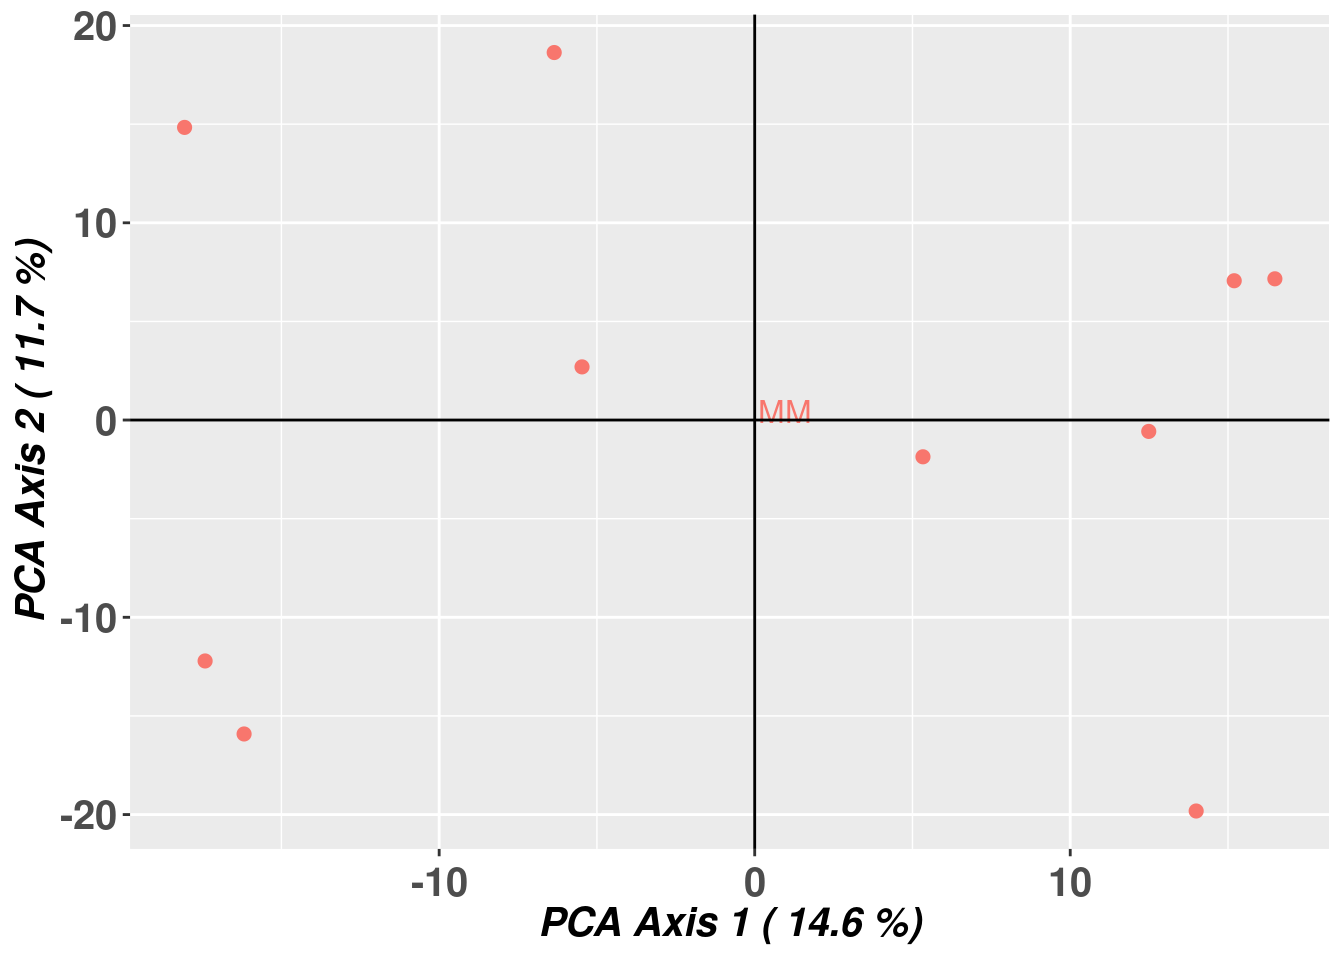
\includegraphics{Session10_SexLinkedMarkers_files/figure-pdf/unnamed-chunk-7-2.pdf}

}

\end{figure}

\begin{figure}[H]

{\centering 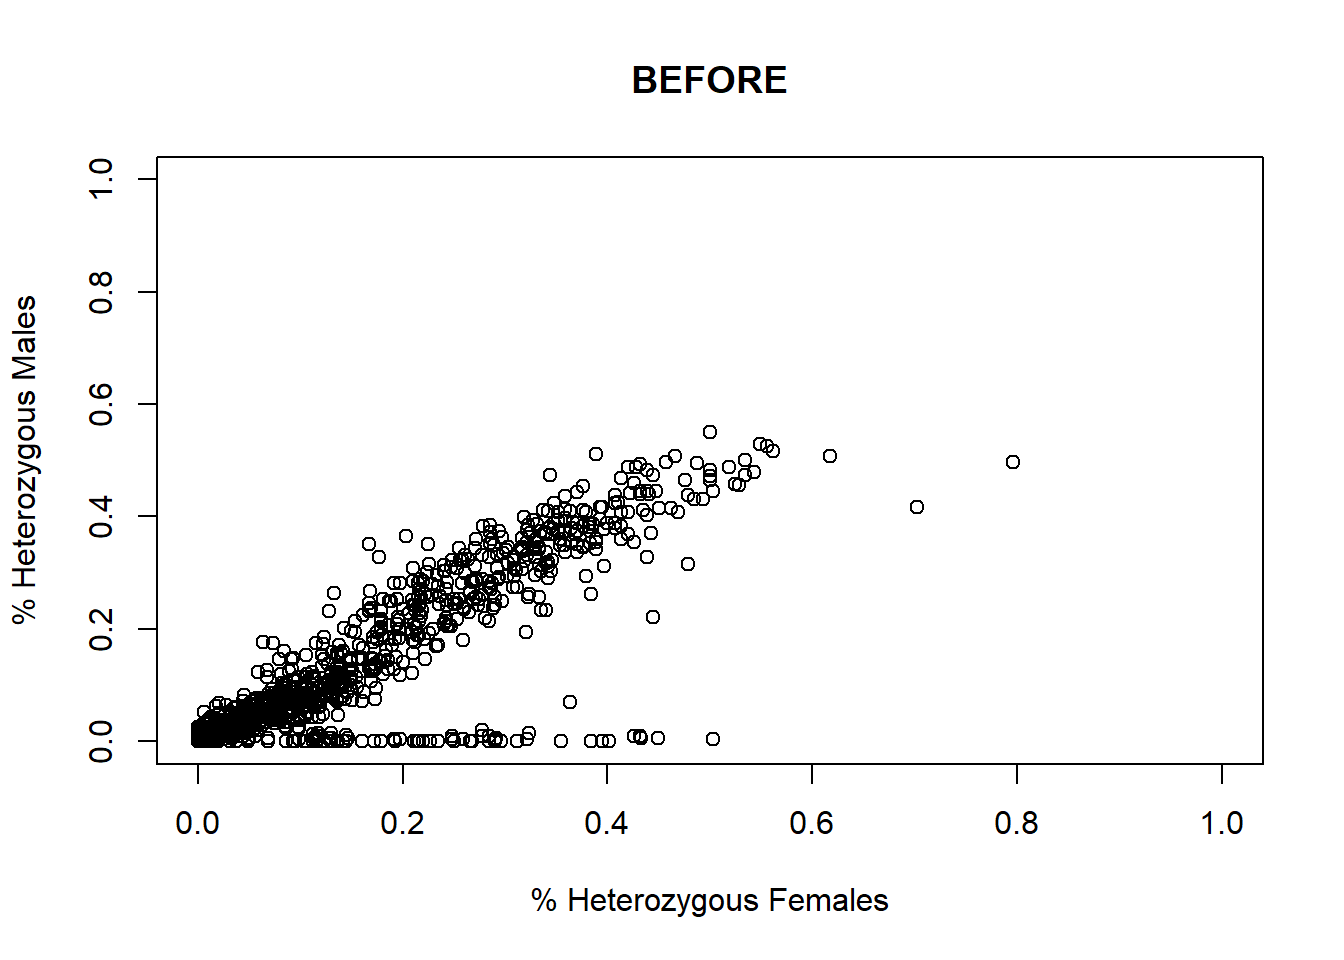
\includegraphics{Session10_SexLinkedMarkers_files/figure-pdf/unnamed-chunk-7-3.pdf}

}

\end{figure}

\begin{verbatim}
Done building heterozygosity plots.
\end{verbatim}

\begin{verbatim}
**FINISHED** Total of analyzed loci: 1000.
Found 77 sex-linked loci:
   1 Y-linked loci
   9 sex-biased loci
   66 X-linked loci
   1 XY gametologs.
And 923 autosomal loci.
\end{verbatim}

\begin{figure}[H]

{\centering 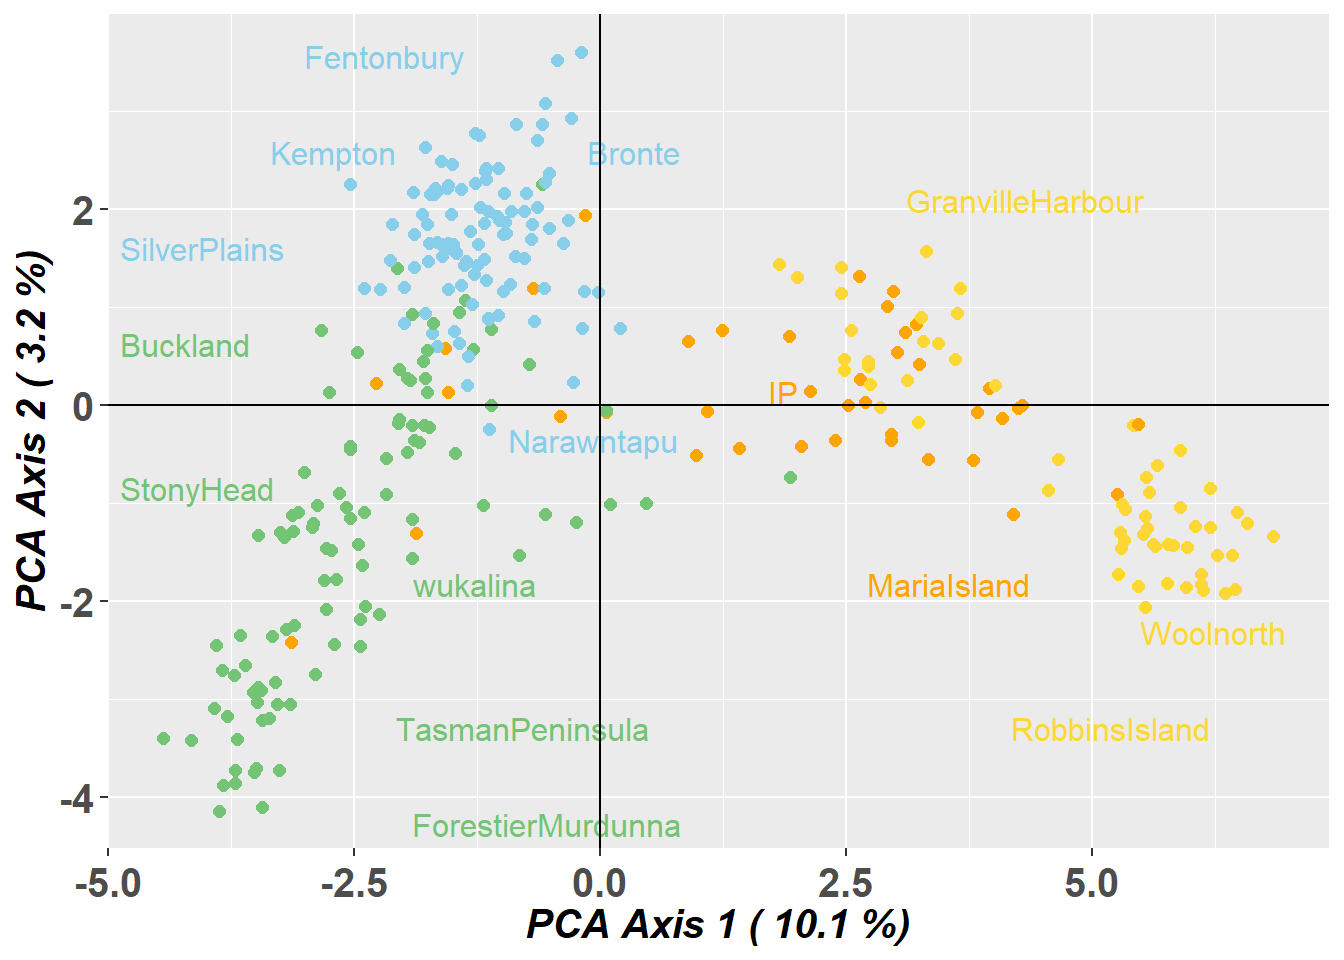
\includegraphics{Session10_SexLinkedMarkers_files/figure-pdf/unnamed-chunk-7-4.pdf}

}

\end{figure}

\begin{tcolorbox}[enhanced jigsaw, coltitle=black, colframe=quarto-callout-note-color-frame, colbacktitle=quarto-callout-note-color!10!white, breakable, bottomtitle=1mm, rightrule=.15mm, opacitybacktitle=0.6, left=2mm, arc=.35mm, opacityback=0, leftrule=.75mm, toptitle=1mm, titlerule=0mm, title=\textcolor{quarto-callout-note-color}{\faInfo}\hspace{0.5em}{Exercise}, bottomrule=.15mm, toprule=.15mm, colback=white]


\includegraphics[width=0.5in,height=0.5in]{images/task.png}

How many males and females does the dataset contain?

How many sex-linked loci were found?

\end{tcolorbox}

Now check the output:

\begin{Shaded}
\begin{Highlighting}[]
\NormalTok{res}\SpecialCharTok{$}\NormalTok{y.linked  }\CommentTok{\# Notice that it says \textquotesingle{}y{-}linked\textquotesingle{}}
\end{Highlighting}
\end{Shaded}

\begin{verbatim}
 ********************
 *** DARTR OBJECT ***
 ********************

 ** 376 genotypes,  1 SNPs , size: 4.7 Mb

    missing data: 164 (=43.62 %) scored as NA

 ** Genetic data
   @gen: list of 376 SNPbin
   @ploidy: ploidy of each individual  (range: 2-2)

 ** Additional data
   @ind.names:  376 individual labels
   @loc.names:  1 locus labels
   @loc.all:  1 allele labels
   @position: integer storing positions of the SNPs [within 69 base sequence]
   @pop: population of each individual (group size range: 95-281)
   @other: a list containing: loc.metrics, ind.metrics, loc.metrics.flags, verbose, history 
    @other$ind.metrics: id, sex, pop, Year.collected, service, plate_location 
    @other$loc.metrics: AlleleID, CloneID, AlleleSequence, TrimmedSequence, Chrom_Possum_v2, ChromPos_Possum_v2, AlnCnt_Possum_v2, AlnEvalue_Possum_v2, SNP, SnpPosition, CallRate, OneRatioRef, OneRatioSnp, FreqHomRef, FreqHomSnp, FreqHets, PICRef, PICSnp, AvgPIC, AvgCountRef, AvgCountSnp, RepAvg, clone, uid, rdepth, monomorphs, maf, OneRatio, PIC 
   @other$latlon[g]: no coordinates attached
\end{verbatim}

\begin{Shaded}
\begin{Highlighting}[]
\NormalTok{res}\SpecialCharTok{$}\NormalTok{x.linked  }\CommentTok{\# Notice that it says \textquotesingle{}x{-}linked\textquotesingle{}}
\end{Highlighting}
\end{Shaded}

\begin{verbatim}
 ********************
 *** DARTR OBJECT ***
 ********************

 ** 376 genotypes,  66 SNPs , size: 4.7 Mb

    missing data: 827 (=3.33 %) scored as NA

 ** Genetic data
   @gen: list of 376 SNPbin
   @ploidy: ploidy of each individual  (range: 2-2)

 ** Additional data
   @ind.names:  376 individual labels
   @loc.names:  66 locus labels
   @loc.all:  66 allele labels
   @position: integer storing positions of the SNPs [within 69 base sequence]
   @pop: population of each individual (group size range: 95-281)
   @other: a list containing: loc.metrics, ind.metrics, loc.metrics.flags, verbose, history 
    @other$ind.metrics: id, sex, pop, Year.collected, service, plate_location 
    @other$loc.metrics: AlleleID, CloneID, AlleleSequence, TrimmedSequence, Chrom_Possum_v2, ChromPos_Possum_v2, AlnCnt_Possum_v2, AlnEvalue_Possum_v2, SNP, SnpPosition, CallRate, OneRatioRef, OneRatioSnp, FreqHomRef, FreqHomSnp, FreqHets, PICRef, PICSnp, AvgPIC, AvgCountRef, AvgCountSnp, RepAvg, clone, uid, rdepth, monomorphs, maf, OneRatio, PIC 
   @other$latlon[g]: no coordinates attached
\end{verbatim}

\begin{Shaded}
\begin{Highlighting}[]
\NormalTok{res}\SpecialCharTok{$}\NormalTok{gametolog}
\end{Highlighting}
\end{Shaded}

\begin{verbatim}
 ********************
 *** DARTR OBJECT ***
 ********************

 ** 376 genotypes,  1 SNPs , size: 4.7 Mb

    missing data: 0 (=0 %) scored as NA

 ** Genetic data
   @gen: list of 376 SNPbin
   @ploidy: ploidy of each individual  (range: 2-2)

 ** Additional data
   @ind.names:  376 individual labels
   @loc.names:  1 locus labels
   @loc.all:  1 allele labels
   @position: integer storing positions of the SNPs [within 69 base sequence]
   @pop: population of each individual (group size range: 95-281)
   @other: a list containing: loc.metrics, ind.metrics, loc.metrics.flags, verbose, history 
    @other$ind.metrics: id, sex, pop, Year.collected, service, plate_location 
    @other$loc.metrics: AlleleID, CloneID, AlleleSequence, TrimmedSequence, Chrom_Possum_v2, ChromPos_Possum_v2, AlnCnt_Possum_v2, AlnEvalue_Possum_v2, SNP, SnpPosition, CallRate, OneRatioRef, OneRatioSnp, FreqHomRef, FreqHomSnp, FreqHets, PICRef, PICSnp, AvgPIC, AvgCountRef, AvgCountSnp, RepAvg, clone, uid, rdepth, monomorphs, maf, OneRatio, PIC 
   @other$latlon[g]: no coordinates attached
\end{verbatim}

\begin{Shaded}
\begin{Highlighting}[]
\NormalTok{res}\SpecialCharTok{$}\NormalTok{sex.biased}
\end{Highlighting}
\end{Shaded}

\begin{verbatim}
 ********************
 *** DARTR OBJECT ***
 ********************

 ** 376 genotypes,  9 SNPs , size: 4.7 Mb

    missing data: 853 (=25.21 %) scored as NA

 ** Genetic data
   @gen: list of 376 SNPbin
   @ploidy: ploidy of each individual  (range: 2-2)

 ** Additional data
   @ind.names:  376 individual labels
   @loc.names:  9 locus labels
   @loc.all:  9 allele labels
   @position: integer storing positions of the SNPs [within 69 base sequence]
   @pop: population of each individual (group size range: 95-281)
   @other: a list containing: loc.metrics, ind.metrics, loc.metrics.flags, verbose, history 
    @other$ind.metrics: id, sex, pop, Year.collected, service, plate_location 
    @other$loc.metrics: AlleleID, CloneID, AlleleSequence, TrimmedSequence, Chrom_Possum_v2, ChromPos_Possum_v2, AlnCnt_Possum_v2, AlnEvalue_Possum_v2, SNP, SnpPosition, CallRate, OneRatioRef, OneRatioSnp, FreqHomRef, FreqHomSnp, FreqHets, PICRef, PICSnp, AvgPIC, AvgCountRef, AvgCountSnp, RepAvg, clone, uid, rdepth, monomorphs, maf, OneRatio, PIC 
   @other$latlon[g]: no coordinates attached
\end{verbatim}

\begin{Shaded}
\begin{Highlighting}[]
\NormalTok{res}\SpecialCharTok{$}\NormalTok{autosomal}
\end{Highlighting}
\end{Shaded}

\begin{verbatim}
 ********************
 *** DARTR OBJECT ***
 ********************

 ** 376 genotypes,  923 SNPs , size: 5.2 Mb

    missing data: 18826 (=5.42 %) scored as NA

 ** Genetic data
   @gen: list of 376 SNPbin
   @ploidy: ploidy of each individual  (range: 2-2)

 ** Additional data
   @ind.names:  376 individual labels
   @loc.names:  923 locus labels
   @loc.all:  923 allele labels
   @position: integer storing positions of the SNPs [within 69 base sequence]
   @pop: population of each individual (group size range: 95-281)
   @other: a list containing: loc.metrics, ind.metrics, loc.metrics.flags, verbose, history 
    @other$ind.metrics: id, sex, pop, Year.collected, service, plate_location 
    @other$loc.metrics: AlleleID, CloneID, AlleleSequence, TrimmedSequence, Chrom_Possum_v2, ChromPos_Possum_v2, AlnCnt_Possum_v2, AlnEvalue_Possum_v2, SNP, SnpPosition, CallRate, OneRatioRef, OneRatioSnp, FreqHomRef, FreqHomSnp, FreqHets, PICRef, PICSnp, AvgPIC, AvgCountRef, AvgCountSnp, RepAvg, clone, uid, rdepth, monomorphs, maf, OneRatio, PIC 
   @other$latlon[g]: no coordinates attached
\end{verbatim}

\begin{Shaded}
\begin{Highlighting}[]
\NormalTok{knitr}\SpecialCharTok{::}\FunctionTok{kable}\NormalTok{(}\FunctionTok{head}\NormalTok{(res}\SpecialCharTok{$}\NormalTok{results.table))  }\CommentTok{\# The output table}
\end{Highlighting}
\end{Shaded}

\begin{longtable}[]{@{}
  >{\raggedright\arraybackslash}p{(\columnwidth - 46\tabcolsep) * \real{0.0535}}
  >{\raggedleft\arraybackslash}p{(\columnwidth - 46\tabcolsep) * \real{0.0201}}
  >{\raggedleft\arraybackslash}p{(\columnwidth - 46\tabcolsep) * \real{0.0435}}
  >{\raggedleft\arraybackslash}p{(\columnwidth - 46\tabcolsep) * \real{0.0435}}
  >{\raggedleft\arraybackslash}p{(\columnwidth - 46\tabcolsep) * \real{0.0502}}
  >{\raggedleft\arraybackslash}p{(\columnwidth - 46\tabcolsep) * \real{0.0502}}
  >{\raggedleft\arraybackslash}p{(\columnwidth - 46\tabcolsep) * \real{0.0334}}
  >{\raggedleft\arraybackslash}p{(\columnwidth - 46\tabcolsep) * \real{0.0334}}
  >{\raggedleft\arraybackslash}p{(\columnwidth - 46\tabcolsep) * \real{0.0368}}
  >{\raggedleft\arraybackslash}p{(\columnwidth - 46\tabcolsep) * \real{0.0468}}
  >{\raggedleft\arraybackslash}p{(\columnwidth - 46\tabcolsep) * \real{0.0468}}
  >{\raggedright\arraybackslash}p{(\columnwidth - 46\tabcolsep) * \real{0.0301}}
  >{\raggedright\arraybackslash}p{(\columnwidth - 46\tabcolsep) * \real{0.0368}}
  >{\raggedleft\arraybackslash}p{(\columnwidth - 46\tabcolsep) * \real{0.0401}}
  >{\raggedleft\arraybackslash}p{(\columnwidth - 46\tabcolsep) * \real{0.0401}}
  >{\raggedleft\arraybackslash}p{(\columnwidth - 46\tabcolsep) * \real{0.0401}}
  >{\raggedleft\arraybackslash}p{(\columnwidth - 46\tabcolsep) * \real{0.0401}}
  >{\raggedleft\arraybackslash}p{(\columnwidth - 46\tabcolsep) * \real{0.0301}}
  >{\raggedleft\arraybackslash}p{(\columnwidth - 46\tabcolsep) * \real{0.0435}}
  >{\raggedleft\arraybackslash}p{(\columnwidth - 46\tabcolsep) * \real{0.0535}}
  >{\raggedleft\arraybackslash}p{(\columnwidth - 46\tabcolsep) * \real{0.0569}}
  >{\raggedleft\arraybackslash}p{(\columnwidth - 46\tabcolsep) * \real{0.0569}}
  >{\raggedright\arraybackslash}p{(\columnwidth - 46\tabcolsep) * \real{0.0301}}
  >{\raggedright\arraybackslash}p{(\columnwidth - 46\tabcolsep) * \real{0.0435}}@{}}
\toprule\noalign{}
\begin{minipage}[b]{\linewidth}\raggedright
\end{minipage} & \begin{minipage}[b]{\linewidth}\raggedleft
index
\end{minipage} & \begin{minipage}[b]{\linewidth}\raggedleft
count.F.miss
\end{minipage} & \begin{minipage}[b]{\linewidth}\raggedleft
count.M.miss
\end{minipage} & \begin{minipage}[b]{\linewidth}\raggedleft
count.F.scored
\end{minipage} & \begin{minipage}[b]{\linewidth}\raggedleft
count.M.scored
\end{minipage} & \begin{minipage}[b]{\linewidth}\raggedleft
ratio
\end{minipage} & \begin{minipage}[b]{\linewidth}\raggedleft
p.value
\end{minipage} & \begin{minipage}[b]{\linewidth}\raggedleft
p.adjusted
\end{minipage} & \begin{minipage}[b]{\linewidth}\raggedleft
scoringRate.F
\end{minipage} & \begin{minipage}[b]{\linewidth}\raggedleft
scoringRate.M
\end{minipage} & \begin{minipage}[b]{\linewidth}\raggedright
y.linked
\end{minipage} & \begin{minipage}[b]{\linewidth}\raggedright
sex.biased
\end{minipage} & \begin{minipage}[b]{\linewidth}\raggedleft
count.F.het
\end{minipage} & \begin{minipage}[b]{\linewidth}\raggedleft
count.M.het
\end{minipage} & \begin{minipage}[b]{\linewidth}\raggedleft
count.F.hom
\end{minipage} & \begin{minipage}[b]{\linewidth}\raggedleft
count.M.hom
\end{minipage} & \begin{minipage}[b]{\linewidth}\raggedleft
stat
\end{minipage} & \begin{minipage}[b]{\linewidth}\raggedleft
stat.p.value
\end{minipage} & \begin{minipage}[b]{\linewidth}\raggedleft
stat.p.adjusted
\end{minipage} & \begin{minipage}[b]{\linewidth}\raggedleft
heterozygosity.F
\end{minipage} & \begin{minipage}[b]{\linewidth}\raggedleft
heterozygosity.M
\end{minipage} & \begin{minipage}[b]{\linewidth}\raggedright
x.linked
\end{minipage} & \begin{minipage}[b]{\linewidth}\raggedright
xy.gametolog
\end{minipage} \\
\midrule\noalign{}
\endhead
\bottomrule\noalign{}
\endlastfoot
28681424-34-G/T & 1 & 0 & 1 & 162 & 210 & 1.2953770 & 1.0000000 & 1 &
1.0000000 & 0.9952607 & FALSE & FALSE & 1 & 0 & 161 & 210 & 1.303397 &
1.0000000 & 1.0000000 & 0.0061728 & 0.0000000 & FALSE & FALSE \\
28678947-56-C/T & 2 & 12 & 8 & 150 & 203 & 2.0261283 & 0.1638428 & 1 &
0.9259259 & 0.9620853 & FALSE & FALSE & 9 & 7 & 141 & 196 & 1.784196 &
0.3044519 & 0.9598961 & 0.0600000 & 0.0344828 & FALSE & FALSE \\
28680567-32-T/G & 3 & 12 & 12 & 150 & 199 & 1.3256351 & 0.5289429 & 1 &
0.9259259 & 0.9431280 & FALSE & FALSE & 9 & 11 & 141 & 188 & 1.090635 &
1.0000000 & 1.0000000 & 0.0600000 & 0.0552764 & FALSE & FALSE \\
28688313-7-C/G & 4 & 0 & 0 & 162 & 211 & 1.3015303 & 1.0000000 & 1 &
1.0000000 & 1.0000000 & FALSE & FALSE & 6 & 0 & 156 & 211 & 8.076192 &
0.0459068 & 0.3917911 & 0.0370370 & 0.0000000 & FALSE & FALSE \\
28681679-51-C/T & 5 & 22 & 30 & 140 & 181 & 0.9482168 & 0.8814171 & 1 &
0.8641975 & 0.8578199 & FALSE & FALSE & 1 & 1 & 139 & 180 & 1.293900 &
1.0000000 & 1.0000000 & 0.0071429 & 0.0055249 & FALSE & FALSE \\
28681994-14-G/A & 6 & 0 & 1 & 162 & 210 & 1.2953770 & 1.0000000 & 1 &
1.0000000 & 0.9952607 & FALSE & FALSE & 18 & 19 & 144 & 191 & 1.255791 &
0.6007790 & 1.0000000 & 0.1111111 & 0.0904762 & FALSE & FALSE \\
\end{longtable}

The output consists of a genlight object for each type of loci, plus a
results table.

\hypertarget{run-infer.sex-1}{%
\section*{\texorpdfstring{Run
\texttt{infer.sex}}{Run infer.sex}}\label{run-infer.sex-1}}
\addcontentsline{toc}{section}{Run \texttt{infer.sex}}

\markright{Run \texttt{infer.sex}}

This function uses the output of function filter.sex.linked (list of 6
objects) to infer the sex of all individuals in the dataset. It uses 3
types of sex-linked loci (W-/Y-linked, Z-/X-linked, and gametologs),
assigns a preliminary genetic sex for each type of sex-linked loci
available, and outputs an \texttt{agreed\ sex}.

\begin{Shaded}
\begin{Highlighting}[]
\NormalTok{sexID }\OtherTok{\textless{}{-}}\NormalTok{ dartR.sexlinked}\SpecialCharTok{::}\FunctionTok{infer.sex}\NormalTok{(}\AttributeTok{gl\_sex\_filtered =}\NormalTok{ res, }\AttributeTok{system =} \StringTok{"xy"}\NormalTok{,}
    \AttributeTok{seed =} \DecValTok{124}\NormalTok{)}
\end{Highlighting}
\end{Shaded}

\begin{verbatim}
Not enough gametologs (need at least 5). Assigning NA...
\end{verbatim}

\begin{verbatim}
***FINISHED***
\end{verbatim}

\begin{Shaded}
\begin{Highlighting}[]
\NormalTok{knitr}\SpecialCharTok{::}\FunctionTok{kable}\NormalTok{(}\FunctionTok{head}\NormalTok{(sexID))}
\end{Highlighting}
\end{Shaded}

\begin{longtable}[]{@{}
  >{\raggedright\arraybackslash}p{(\columnwidth - 22\tabcolsep) * \real{0.0385}}
  >{\raggedright\arraybackslash}p{(\columnwidth - 22\tabcolsep) * \real{0.0385}}
  >{\raggedright\arraybackslash}p{(\columnwidth - 22\tabcolsep) * \real{0.1250}}
  >{\raggedleft\arraybackslash}p{(\columnwidth - 22\tabcolsep) * \real{0.0769}}
  >{\raggedleft\arraybackslash}p{(\columnwidth - 22\tabcolsep) * \real{0.0865}}
  >{\raggedright\arraybackslash}p{(\columnwidth - 22\tabcolsep) * \real{0.1250}}
  >{\raggedleft\arraybackslash}p{(\columnwidth - 22\tabcolsep) * \real{0.0673}}
  >{\raggedleft\arraybackslash}p{(\columnwidth - 22\tabcolsep) * \real{0.0673}}
  >{\raggedright\arraybackslash}p{(\columnwidth - 22\tabcolsep) * \real{0.1346}}
  >{\raggedright\arraybackslash}p{(\columnwidth - 22\tabcolsep) * \real{0.0673}}
  >{\raggedright\arraybackslash}p{(\columnwidth - 22\tabcolsep) * \real{0.0673}}
  >{\raggedright\arraybackslash}p{(\columnwidth - 22\tabcolsep) * \real{0.1058}}@{}}
\toprule\noalign{}
\begin{minipage}[b]{\linewidth}\raggedright
\end{minipage} & \begin{minipage}[b]{\linewidth}\raggedright
id
\end{minipage} & \begin{minipage}[b]{\linewidth}\raggedright
y.linked.sex
\end{minipage} & \begin{minipage}[b]{\linewidth}\raggedleft
\#called
\end{minipage} & \begin{minipage}[b]{\linewidth}\raggedleft
\#missing
\end{minipage} & \begin{minipage}[b]{\linewidth}\raggedright
x.linked.sex
\end{minipage} & \begin{minipage}[b]{\linewidth}\raggedleft
\#Het.x
\end{minipage} & \begin{minipage}[b]{\linewidth}\raggedleft
\#Hom.x
\end{minipage} & \begin{minipage}[b]{\linewidth}\raggedright
gametolog.sex
\end{minipage} & \begin{minipage}[b]{\linewidth}\raggedright
\#Het.g
\end{minipage} & \begin{minipage}[b]{\linewidth}\raggedright
\#Hom.g
\end{minipage} & \begin{minipage}[b]{\linewidth}\raggedright
agreed.sex
\end{minipage} \\
\midrule\noalign{}
\endhead
\bottomrule\noalign{}
\endlastfoot
Y2 & Y2 & F & 0 & 1 & F & 19 & 47 & NA & NA & NA & F \\
Y16 & Y16 & M & 1 & 0 & M & 2 & 56 & NA & NA & NA & M \\
Y17 & Y17 & F & 0 & 1 & F & 27 & 37 & NA & NA & NA & F \\
Y18 & Y18 & F & 0 & 1 & M & 4 & 62 & NA & NA & NA & *F \\
Y3 & Y3 & M & 1 & 0 & M & 3 & 63 & NA & NA & NA & M \\
Y4 & Y4 & M & 1 & 0 & M & 1 & 63 & NA & NA & NA & M \\
\end{longtable}

What did the function mention about gametologs? How did that impact the
results table? How many types of sex-linked loci were used to infer an
\texttt{agreed\ sex}?

\begin{tcolorbox}[enhanced jigsaw, coltitle=black, colframe=quarto-callout-note-color-frame, colbacktitle=quarto-callout-note-color!10!white, breakable, bottomtitle=1mm, rightrule=.15mm, opacitybacktitle=0.6, left=2mm, arc=.35mm, opacityback=0, leftrule=.75mm, toptitle=1mm, titlerule=0mm, title=\textcolor{quarto-callout-note-color}{\faInfo}\hspace{0.5em}{Exercise}, bottomrule=.15mm, toprule=.15mm, colback=white]


\includegraphics[width=0.5in,height=0.5in]{images/task.png}

Can you find individuals for which the \texttt{agreed\ sex} is uncertain
(i.e., has an asterisk ``*'')?

\end{tcolorbox}

\bookmarksetup{startatroot}

\hypertarget{exercise-10}{%
\chapter*{EXERCISE}\label{exercise-10}}
\addcontentsline{toc}{chapter}{EXERCISE}

\markboth{EXERCISE}{EXERCISE}

\begin{tcolorbox}[enhanced jigsaw, coltitle=black, colframe=quarto-callout-note-color-frame, colbacktitle=quarto-callout-note-color!10!white, breakable, bottomtitle=1mm, rightrule=.15mm, opacitybacktitle=0.6, left=2mm, arc=.35mm, opacityback=0, leftrule=.75mm, toptitle=1mm, titlerule=0mm, title=\textcolor{quarto-callout-note-color}{\faInfo}\hspace{0.5em}{Exercise}, bottomrule=.15mm, toprule=.15mm, colback=white]


\includegraphics[width=0.5in,height=0.5in]{images/task.png}

Imagine you are analyzing the genetic data of a population and you want
to look at its genetic structure and genetic diversity. You get to work
by filtering your beautiful set of SNPs. Because you are a rigorous, you
want to test whether using function \texttt{filter.sex.linked} to
properly filter out sex-linked loci changes the results of the
populations analyses. So you: (1) process your SNP dataset by applying
standard filters and run analyses, and (2) process the dataset by
filtering out sex-linked loci first, applying standard filters second,
and then run analyses.

Choose one of the following datasets (or your own data) and report:

\begin{enumerate}
\def\labelenumi{\arabic{enumi}.}
\item
  How many sex-linked markers are present?
\item
  How many individuals had a wrong sexID?
\item
  Do you see any changes in your PCA/structure analyses when you
  filtered out sex-linked markers versus when you did not?
\item
  Do you see any differences in genetic diversity and fixation indices
  when you filtered out sex-linked markers versus when you did not?
\end{enumerate}

\end{tcolorbox}


\includegraphics[width=3.64583in,height=2.08333in]{images/beer.png}
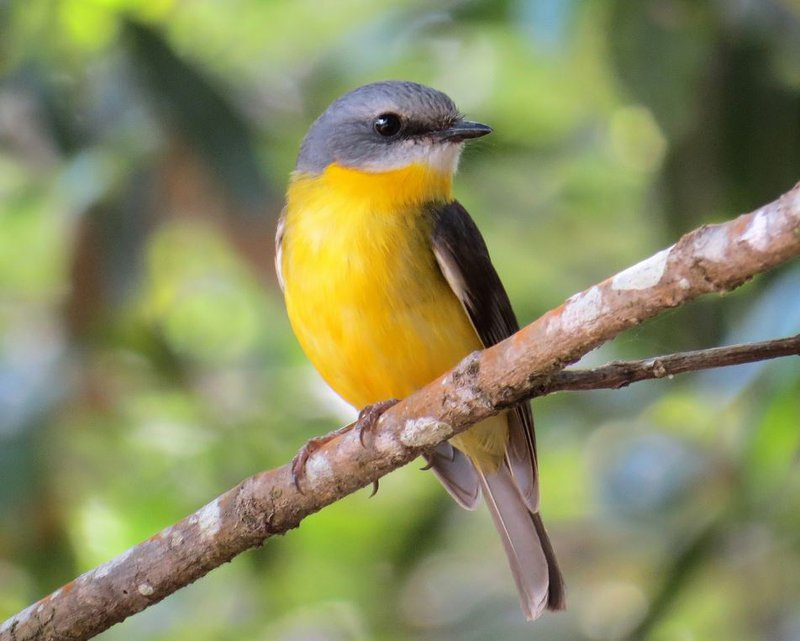
\includegraphics[width=3.63542in,height=\textheight]{images/Eastern_Yellow_Robin.jpg}

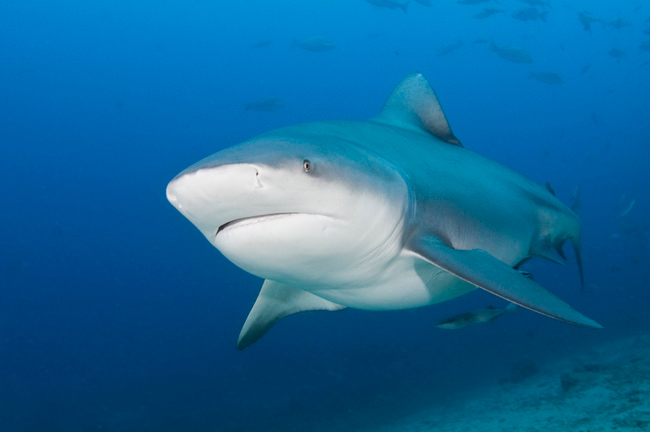
\includegraphics[width=3.64583in,height=2.08333in]{images/Bull_Shark.jpg}
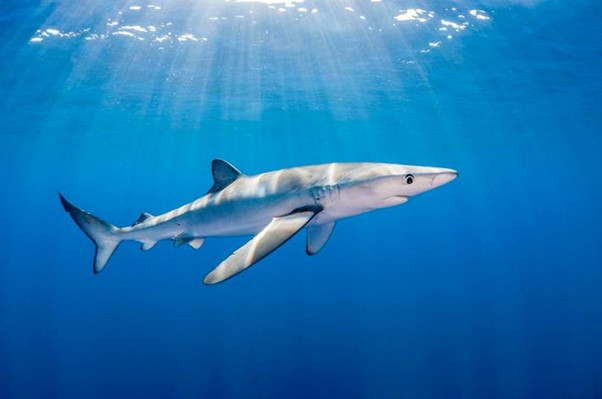
\includegraphics[width=3.64583in,height=2.08333in]{images/Blue_shark.jpg}

\hypertarget{exercise-data-1---your-own-data}{%
\section*{Exercise data 1 - Your own
data}\label{exercise-data-1---your-own-data}}
\addcontentsline{toc}{section}{Exercise data 1 - Your own data}

\markright{Exercise data 1 - Your own data}

\begin{infobox}{task}
\textbf{HINT}

You can have a look at the exercise data below for inspiration.

\end{infobox}

\hypertarget{number-of-sex-linked-markers}{%
\subsection*{1. Number of sex-linked
markers?}\label{number-of-sex-linked-markers}}
\addcontentsline{toc}{subsection}{1. Number of sex-linked markers?}

\hypertarget{individuals-with-wrong-sexid}{%
\subsection*{2. Individuals with wrong
sexID?}\label{individuals-with-wrong-sexid}}
\addcontentsline{toc}{subsection}{2. Individuals with wrong sexID?}

\hypertarget{changes-in-pca-before-and-after-removing-the-slm}{%
\subsection*{3. Changes in PCA before and after removing the
SLM?}\label{changes-in-pca-before-and-after-removing-the-slm}}
\addcontentsline{toc}{subsection}{3. Changes in PCA before and after
removing the SLM?}

\hypertarget{differences-in-genetic-diversity-and-fixation-indices-between-autosomal-and-slm}{%
\subsection*{4. Differences in genetic diversity and fixation indices
between autosomal and
SLM?}\label{differences-in-genetic-diversity-and-fixation-indices-between-autosomal-and-slm}}
\addcontentsline{toc}{subsection}{4. Differences in genetic diversity
and fixation indices between autosomal and SLM?}

\hypertarget{exercise-data-2---the-eastern-yellow-robin}{%
\section*{Exercise data 2 - The Eastern Yellow
Robin}\label{exercise-data-2---the-eastern-yellow-robin}}
\addcontentsline{toc}{section}{Exercise data 2 - The Eastern Yellow
Robin}

\markright{Exercise data 2 - The Eastern Yellow Robin}

Data from Robledo-Ruiz et al.~2023.

\begin{figure}

{\centering 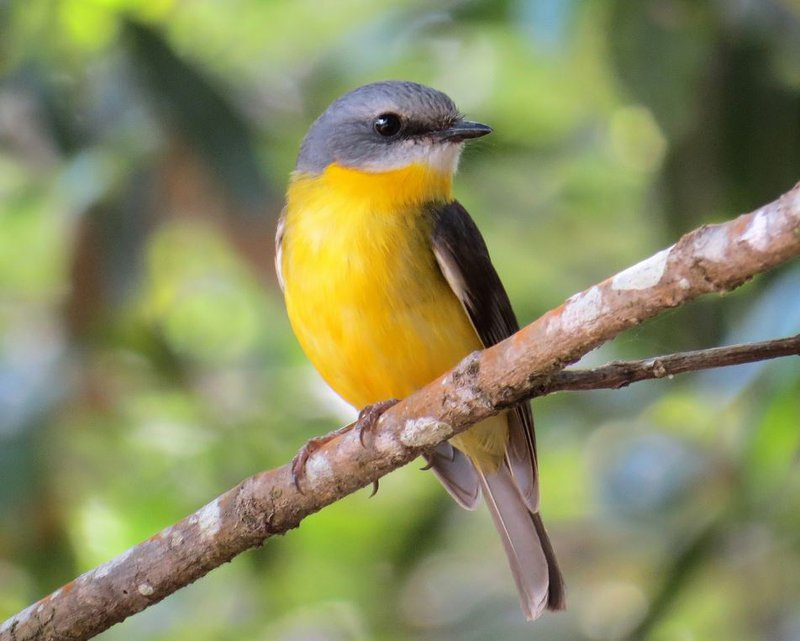
\includegraphics{images/Eastern_Yellow_Robin.jpg}

}

\caption{The Eastern Yellow Robin}

\end{figure}

\hypertarget{load-data-2}{%
\subsection*{Load data}\label{load-data-2}}
\addcontentsline{toc}{subsection}{Load data}

\begin{Shaded}
\begin{Highlighting}[]
\FunctionTok{data}\NormalTok{(}\StringTok{"EYR"}\NormalTok{)}

\NormalTok{EYR}\SpecialCharTok{@}\NormalTok{n.loc}
\FunctionTok{table}\NormalTok{(EYR}\SpecialCharTok{@}\NormalTok{pop)}
\FunctionTok{table}\NormalTok{(EYR}\SpecialCharTok{@}\NormalTok{other}\SpecialCharTok{$}\NormalTok{ind.metrics}\SpecialCharTok{$}\NormalTok{pop)}
\FunctionTok{table}\NormalTok{(EYR}\SpecialCharTok{@}\NormalTok{other}\SpecialCharTok{$}\NormalTok{ind.metrics}\SpecialCharTok{$}\NormalTok{sex, }\AttributeTok{useNA =} \StringTok{"ifany"}\NormalTok{)}
\end{Highlighting}
\end{Shaded}

\begin{verbatim}
[1] 1000

    Crusoe Muckleford      Timor     Wombat 
       238        421         52         71 

    Crusoe Muckleford      Timor     Wombat 
       238        421         52         71 

      F   M 
  1 352 429 
\end{verbatim}

\hypertarget{number-of-sex-linked-markers-1}{%
\subsection*{1. Number of sex-linked
markers?}\label{number-of-sex-linked-markers-1}}
\addcontentsline{toc}{subsection}{1. Number of sex-linked markers?}

\begin{Shaded}
\begin{Highlighting}[]
\NormalTok{res }\OtherTok{\textless{}{-}}\NormalTok{ dartR.sexlinked}\SpecialCharTok{::}\FunctionTok{filter.sex.linked}\NormalTok{(}\AttributeTok{gl =}\NormalTok{ EYR, }\AttributeTok{system =} \StringTok{"zw"}\NormalTok{)}
\end{Highlighting}
\end{Shaded}

\begin{verbatim}
Detected 352 females and 429 males.
\end{verbatim}

\begin{verbatim}
Starting phase 1. May take a while...
\end{verbatim}

\begin{verbatim}
Building call rate plots.
\end{verbatim}

\begin{figure}[H]

{\centering \includegraphics{Session10_SexLinkedMarkers_files/figure-pdf/unnamed-chunk-11-1.pdf}

}

\end{figure}

\begin{verbatim}
Done. Starting phase 2.
\end{verbatim}

\begin{verbatim}
Building heterozygosity plots.
\end{verbatim}

\begin{figure}[H]

{\centering 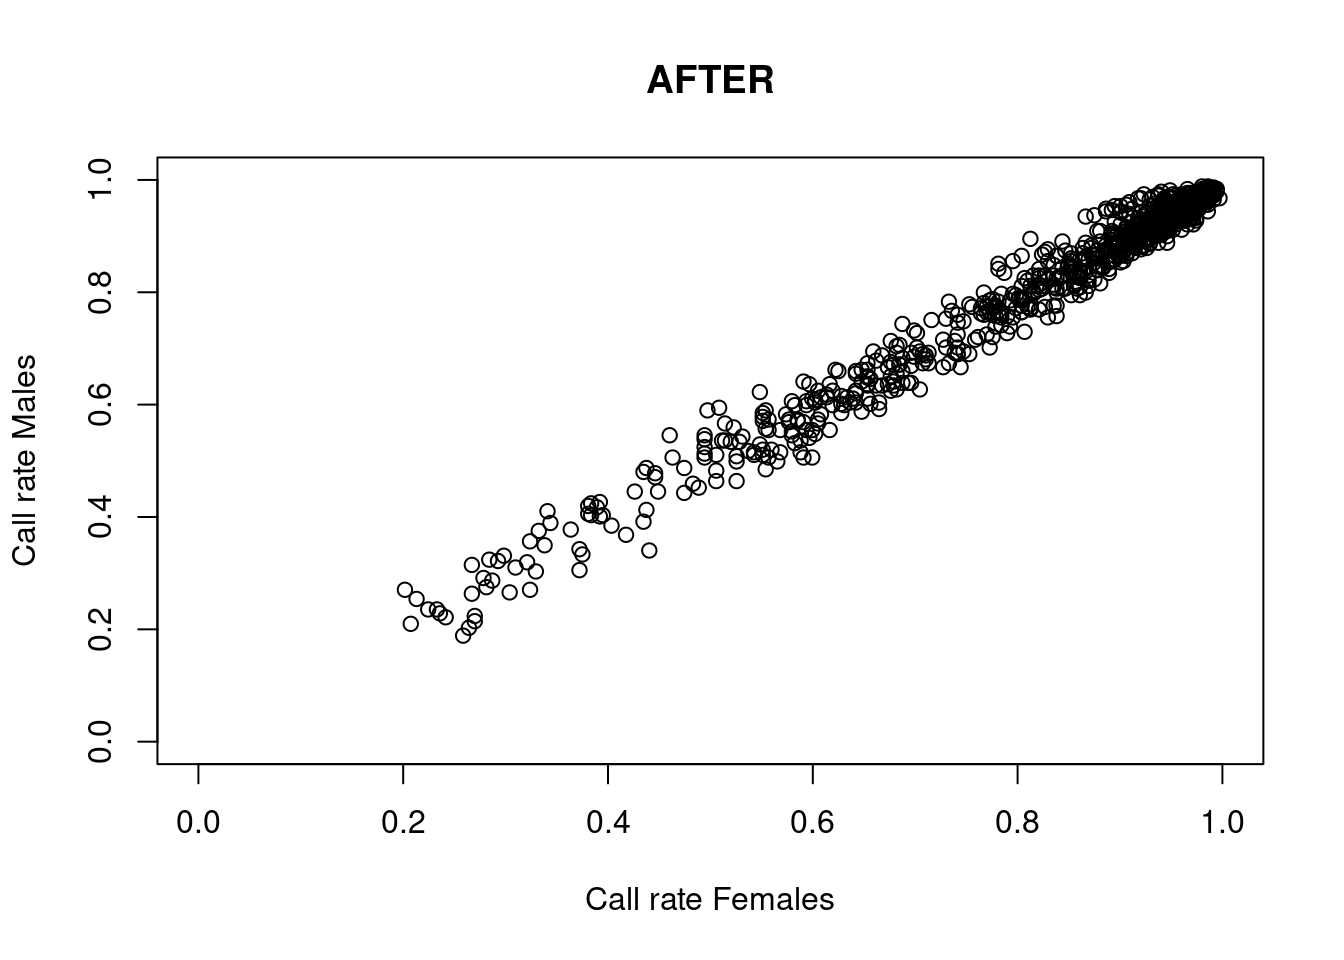
\includegraphics{Session10_SexLinkedMarkers_files/figure-pdf/unnamed-chunk-11-2.pdf}

}

\end{figure}

\begin{figure}[H]

{\centering \includegraphics{Session10_SexLinkedMarkers_files/figure-pdf/unnamed-chunk-11-3.pdf}

}

\end{figure}

\begin{verbatim}
Done building heterozygosity plots.
\end{verbatim}

\begin{verbatim}
**FINISHED** Total of analyzed loci: 1000.
Found 150 sex-linked loci:
   16 W-linked loci
   82 sex-biased loci
   32 Z-linked loci
   20 ZW gametologs.
And 850 autosomal loci.
\end{verbatim}

\begin{figure}[H]

{\centering \includegraphics{Session10_SexLinkedMarkers_files/figure-pdf/unnamed-chunk-11-4.pdf}

}

\end{figure}

\hypertarget{individuals-with-wrong-sexid-1}{%
\subsection*{2. Individuals with wrong
sexID?}\label{individuals-with-wrong-sexid-1}}
\addcontentsline{toc}{subsection}{2. Individuals with wrong sexID?}

\begin{Shaded}
\begin{Highlighting}[]
\NormalTok{sexID }\OtherTok{\textless{}{-}}\NormalTok{ dartR.sexlinked}\SpecialCharTok{::}\FunctionTok{infer.sex}\NormalTok{(}\AttributeTok{gl\_sex\_filtered =}\NormalTok{ res, }\AttributeTok{system =} \StringTok{"zw"}\NormalTok{,}
    \AttributeTok{seed =} \DecValTok{124}\NormalTok{)}
\end{Highlighting}
\end{Shaded}

\begin{verbatim}
***FINISHED***
\end{verbatim}

\begin{Shaded}
\begin{Highlighting}[]
\NormalTok{knitr}\SpecialCharTok{::}\FunctionTok{kable}\NormalTok{(}\FunctionTok{head}\NormalTok{(sexID))}

\FunctionTok{sum}\NormalTok{(EYR}\SpecialCharTok{$}\NormalTok{other}\SpecialCharTok{$}\NormalTok{ind.metrics}\SpecialCharTok{$}\NormalTok{sex }\SpecialCharTok{!=}\NormalTok{ sexID}\SpecialCharTok{$}\NormalTok{agreed.sex, }\AttributeTok{na.rm =} \ConstantTok{TRUE}\NormalTok{)}
\end{Highlighting}
\end{Shaded}

\begin{longtable}[]{@{}
  >{\raggedright\arraybackslash}p{(\columnwidth - 22\tabcolsep) * \real{0.0932}}
  >{\raggedright\arraybackslash}p{(\columnwidth - 22\tabcolsep) * \real{0.0932}}
  >{\raggedright\arraybackslash}p{(\columnwidth - 22\tabcolsep) * \real{0.1102}}
  >{\raggedleft\arraybackslash}p{(\columnwidth - 22\tabcolsep) * \real{0.0763}}
  >{\raggedleft\arraybackslash}p{(\columnwidth - 22\tabcolsep) * \real{0.0678}}
  >{\raggedright\arraybackslash}p{(\columnwidth - 22\tabcolsep) * \real{0.1102}}
  >{\raggedleft\arraybackslash}p{(\columnwidth - 22\tabcolsep) * \real{0.0593}}
  >{\raggedleft\arraybackslash}p{(\columnwidth - 22\tabcolsep) * \real{0.0593}}
  >{\raggedright\arraybackslash}p{(\columnwidth - 22\tabcolsep) * \real{0.1186}}
  >{\raggedleft\arraybackslash}p{(\columnwidth - 22\tabcolsep) * \real{0.0593}}
  >{\raggedleft\arraybackslash}p{(\columnwidth - 22\tabcolsep) * \real{0.0593}}
  >{\raggedright\arraybackslash}p{(\columnwidth - 22\tabcolsep) * \real{0.0932}}@{}}
\toprule\noalign{}
\begin{minipage}[b]{\linewidth}\raggedright
\end{minipage} & \begin{minipage}[b]{\linewidth}\raggedright
id
\end{minipage} & \begin{minipage}[b]{\linewidth}\raggedright
w.linked.sex
\end{minipage} & \begin{minipage}[b]{\linewidth}\raggedleft
\#missing
\end{minipage} & \begin{minipage}[b]{\linewidth}\raggedleft
\#called
\end{minipage} & \begin{minipage}[b]{\linewidth}\raggedright
z.linked.sex
\end{minipage} & \begin{minipage}[b]{\linewidth}\raggedleft
\#Hom.z
\end{minipage} & \begin{minipage}[b]{\linewidth}\raggedleft
\#Het.z
\end{minipage} & \begin{minipage}[b]{\linewidth}\raggedright
gametolog.sex
\end{minipage} & \begin{minipage}[b]{\linewidth}\raggedleft
\#Hom.g
\end{minipage} & \begin{minipage}[b]{\linewidth}\raggedleft
\#Het.g
\end{minipage} & \begin{minipage}[b]{\linewidth}\raggedright
agreed.sex
\end{minipage} \\
\midrule\noalign{}
\endhead
\bottomrule\noalign{}
\endlastfoot
024-96401 & 024-96401 & M & 0 & 16 & M & 7 & 25 & M & 0 & 5 & M \\
024-96401b & 024-96401b & M & 0 & 16 & M & 9 & 21 & M & 0 & 5 & M \\
024-96402 & 024-96402 & F & 15 & 1 & F & 0 & 32 & F & 5 & 0 & F \\
024-96403 & 024-96403 & M & 1 & 15 & M & 11 & 21 & M & 0 & 5 & M \\
024-96404 & 024-96404 & M & 0 & 16 & M & 12 & 20 & M & 0 & 5 & M \\
024-96405 & 024-96405 & M & 0 & 16 & M & 11 & 21 & M & 0 & 5 & M \\
\end{longtable}

\begin{verbatim}
[1] 55
\end{verbatim}

\begin{tcolorbox}[enhanced jigsaw, coltitle=black, colframe=quarto-callout-note-color-frame, colbacktitle=quarto-callout-note-color!10!white, breakable, bottomtitle=1mm, rightrule=.15mm, opacitybacktitle=0.6, left=2mm, arc=.35mm, opacityback=0, leftrule=.75mm, toptitle=1mm, titlerule=0mm, title=\textcolor{quarto-callout-note-color}{\faInfo}\hspace{0.5em}{Exercise}, bottomrule=.15mm, toprule=.15mm, colback=white]

\includegraphics[width=0.5in,height=0.5in]{images/task.png}

Can you tell which misidentified sexes are due to uncertain genetic sex
(indicated with *)?

\textbf{HINT} Try using
\texttt{grep(pattern\ =\ "\textbackslash{}\textbackslash{}*",\ x\ =\ sexID\$agreed.sex)}

\end{tcolorbox}

\hypertarget{processing-snps-with-two-filtering-regimes}{%
\subsubsection*{Processing SNPs with two filtering
regimes}\label{processing-snps-with-two-filtering-regimes}}
\addcontentsline{toc}{subsubsection}{Processing SNPs with two filtering
regimes}

\hypertarget{filtering-snps-only-with-standard-filters-sloppy}{%
\paragraph*{Filtering SNPs only with standard filters
(sloppy)}\label{filtering-snps-only-with-standard-filters-sloppy}}
\addcontentsline{toc}{paragraph}{Filtering SNPs only with standard
filters (sloppy)}

\begin{Shaded}
\begin{Highlighting}[]
\CommentTok{\# Filter for read depth}
\NormalTok{dartR.base}\SpecialCharTok{::}\FunctionTok{gl.report.rdepth}\NormalTok{(EYR)  }\CommentTok{\# This is the initial dataset}
\end{Highlighting}
\end{Shaded}

\begin{verbatim}
Starting :: 
 Starting dartR.base 
 Starting gl.report.rdepth 
  Processing genlight object with SNP data
  Reporting Read Depth by Locus
  No. of loci = 1000 
  No. of individuals = 782 
    Minimum      :  2.6 
    1st quartile :  4.3 
    Median       :  5.6 
    Mean         :  5.9649 
    3r quartile  :  7.325 
    Maximum      :  13.2 
    Missing Rate Overall:  0.19 
\end{verbatim}

\begin{figure}[H]

{\centering \includegraphics{Session10_SexLinkedMarkers_files/figure-pdf/unnamed-chunk-13-1.pdf}

}

\end{figure}

\begin{verbatim}
   Quantile Threshold Retained Percent Filtered Percent
1      100%      13.2        1     0.1      999    99.9
2       95%       9.9       51     5.1      949    94.9
3       90%       9.0      105    10.5      895    89.5
4       85%       8.3      151    15.1      849    84.9
5       80%       7.8      208    20.8      792    79.2
6       75%       7.3      258    25.8      742    74.2
7       70%       6.9      304    30.4      696    69.6
8       65%       6.5      354    35.4      646    64.6
9       60%       6.2      404    40.4      596    59.6
10      55%       5.9      451    45.1      549    54.9
11      50%       5.6      504    50.4      496    49.6
12      45%       5.3      563    56.3      437    43.7
13      40%       5.1      602    60.2      398    39.8
14      35%       4.8      659    65.9      341    34.1
15      30%       4.6      702    70.2      298    29.8
16      25%       4.3      752    75.2      248    24.8
17      20%       4.0      823    82.3      177    17.7
18      15%       3.9      852    85.2      148    14.8
19      10%       3.6      906    90.6       94     9.4
20       5%       3.3      956    95.6       44     4.4
21       0%       2.6     1000   100.0        0     0.0
Completed: :: 
 Completed: dartR.base 
 Completed: gl.report.rdepth 
\end{verbatim}

\begin{Shaded}
\begin{Highlighting}[]
\NormalTok{EYR.sloppy }\OtherTok{\textless{}{-}}\NormalTok{ dartR.base}\SpecialCharTok{::}\FunctionTok{gl.filter.rdepth}\NormalTok{(EYR, }\AttributeTok{lower =} \DecValTok{3}\NormalTok{, }\AttributeTok{upper =} \DecValTok{11}\NormalTok{, }\AttributeTok{verbose =} \DecValTok{0}\NormalTok{)}
\end{Highlighting}
\end{Shaded}

\begin{figure}[H]

{\centering \includegraphics{Session10_SexLinkedMarkers_files/figure-pdf/unnamed-chunk-13-2.pdf}

}

\end{figure}

\begin{Shaded}
\begin{Highlighting}[]
\CommentTok{\# Filter for loci call rate}
\NormalTok{dartR.base}\SpecialCharTok{::}\FunctionTok{gl.report.callrate}\NormalTok{(EYR.sloppy, }\AttributeTok{method =} \StringTok{"loc"}\NormalTok{)}
\end{Highlighting}
\end{Shaded}

\begin{verbatim}
Starting :: 
 Starting dartR.base 
 Starting gl.report.callrate 
  Processing genlight object with SNP data
  Reporting Call Rate by Locus
  No. of loci = 958 
  No. of individuals = 782 
    Minimum      :  0.20844 
    1st quartile :  0.7202688 
    Median       :  0.895141 
    Mean         :  0.8131871 
    3r quartile  :  0.950128 
    Maximum      :  0.988491 
    Missing Rate Overall:  0.1868 
\end{verbatim}

\begin{figure}[H]

{\centering \includegraphics{Session10_SexLinkedMarkers_files/figure-pdf/unnamed-chunk-13-3.pdf}

}

\end{figure}

\begin{verbatim}
Completed: :: 
 Completed: dartR.base 
 Completed: gl.report.callrate 
\end{verbatim}

\begin{Shaded}
\begin{Highlighting}[]
\NormalTok{EYR.sloppy }\OtherTok{\textless{}{-}}\NormalTok{ dartR.base}\SpecialCharTok{::}\FunctionTok{gl.filter.callrate}\NormalTok{(EYR.sloppy, }\AttributeTok{method =} \StringTok{"loc"}\NormalTok{,}
    \AttributeTok{threshold =} \FloatTok{0.75}\NormalTok{, }\AttributeTok{verbose =} \DecValTok{0}\NormalTok{, }\AttributeTok{recalc =} \ConstantTok{TRUE}\NormalTok{)}

\CommentTok{\# Filter for individual call rate}
\NormalTok{dartR.base}\SpecialCharTok{::}\FunctionTok{gl.report.callrate}\NormalTok{(EYR.sloppy, }\AttributeTok{method =} \StringTok{"ind"}\NormalTok{)}
\end{Highlighting}
\end{Shaded}

\begin{verbatim}
Starting :: 
 Starting dartR.base 
 Starting gl.report.callrate 
  Processing genlight object with SNP data

  Reporting Call Rate by Individual
  No. of loci = 703 
  No. of individuals = 782 
    Minimum      :  0.03556188 
    1st quartile :  0.9174964 
    Median       :  0.9416785 
    Mean         :  0.9108097 
    3r quartile  :  0.9573257 
    Maximum      :  0.9829303 
    Missing Rate Overall:  0.0892 

Listing 4 populations and their average CallRates
  Monitor again after filtering
  Population CallRate   N
1     Crusoe   0.9027 238
2 Muckleford   0.9073 421
3      Timor   0.9402  52
4     Wombat   0.9371  71

Listing 20 individuals with the lowest CallRates
  Use this list to see which individuals will be lost on filtering by individual
  Set ind.to.list parameter to see more individuals
   Individual   CallRate
1    M18.29.1 0.03556188
2    M18.18.1 0.03982930
3    M18.47.2 0.06970128
4    C18.16.1 0.07112376
5   027-34168 0.07681366
6    C18.15.2 0.08534851
7    C18.21.2 0.08677098
8    M18.47.3 0.14224751
9    M18.35.2 0.17211949
10   M18.20.3 0.24039829
11   M20.70.2 0.39687055
12   C18.28.1 0.39971550
13   C18.17.2 0.46088193
14  027-34065 0.50640114
15   C18.14.1 0.50640114
16   M20.70.3 0.50782361
17  M20.110.1 0.52347084
18   M19.12.1 0.53342817
19    M19.8.1 0.54907539
20   M20.64.3 0.56045519

)
\end{verbatim}

\begin{figure}[H]

{\centering \includegraphics{Session10_SexLinkedMarkers_files/figure-pdf/unnamed-chunk-13-4.pdf}

}

\end{figure}

\begin{verbatim}
Completed: :: 
 Completed: dartR.base 
 Completed: gl.report.callrate 
\end{verbatim}

\begin{Shaded}
\begin{Highlighting}[]
\NormalTok{EYR.sloppy }\OtherTok{\textless{}{-}}\NormalTok{ dartR.base}\SpecialCharTok{::}\FunctionTok{gl.filter.callrate}\NormalTok{(EYR.sloppy, }\AttributeTok{method =} \StringTok{"ind"}\NormalTok{,}
    \AttributeTok{threshold =} \FloatTok{0.65}\NormalTok{, }\AttributeTok{verbose =} \DecValTok{0}\NormalTok{, }\AttributeTok{recalc =} \ConstantTok{TRUE}\NormalTok{)}
\end{Highlighting}
\end{Shaded}

\begin{Shaded}
\begin{Highlighting}[]
\CommentTok{\# Filter for MAC (= 3)}
\NormalTok{dartR.base}\SpecialCharTok{::}\FunctionTok{gl.report.maf}\NormalTok{(EYR.sloppy)}
\end{Highlighting}
\end{Shaded}

\begin{verbatim}
Starting :: 
 Starting dartR.base 
 Starting gl.report.maf 
  Processing genlight object with SNP data
Starting :: 

 Starting dartR.base 

 Starting gl.report.maf 

  Reporting Minor Allele Frequency (MAF) by Locus for population Crusoe 
  No. of loci = 670 
  No. of individuals = 231 
    Minimum      :  0.0022 
    1st quantile :  0.064825 
    Median       :  0.1582 
    Mean         :  0.1793525 
    3r quantile  :  0.267475 
    Maximum      :  0.4975 
    Missing Rate Overall:  0.08 

  Reporting Minor Allele Frequency (MAF) by Locus for population Muckleford 
  No. of loci = 683 
  No. of individuals = 401 
    Minimum      :  0.0013 
    1st quantile :  0.05875 
    Median       :  0.1404 
    Mean         :  0.172949 
    3r quantile  :  0.2617 
    Maximum      :  0.4985 
    Missing Rate Overall:  0.07 

  Reporting Minor Allele Frequency (MAF) by Locus for population Timor 
  No. of loci = 589 
  No. of individuals = 52 
    Minimum      :  0.0096 
    1st quantile :  0.0673 
    Median       :  0.1667 
    Mean         :  0.1914129 
    3r quantile  :  0.2872 
    Maximum      :  0.5 
    Missing Rate Overall:  0.06 

  Reporting Minor Allele Frequency (MAF) by Locus for population Wombat 
  No. of loci = 627 
  No. of individuals = 71 
    Minimum      :  0.007 
    1st quantile :  0.06385 
    Median       :  0.1449 
    Mean         :  0.1746703 
    3r quantile  :  0.2542 
    Maximum      :  0.5 
    Missing Rate Overall:  0.06 

  Reporting Minor Allele Frequency (MAF) by Locus OVERALL
  No. of loci = 703 
  No. of individuals = 755 
    Minimum      :  3e-04 
    1st quantile :  0.0627 
    Median       :  0.13435 
    Mean         :  0.1696497 
    3r quantile  :  0.246025 
    Maximum      :  0.4991 
    Missing Rate Overall:  0.07 
\end{verbatim}

\begin{figure}[H]

{\centering \includegraphics{Session10_SexLinkedMarkers_files/figure-pdf/unnamed-chunk-13-5.pdf}

}

\end{figure}

\begin{verbatim}
   Quantile Threshold Retained Percent Filtered Percent
1      100%    0.4991        1     0.1      699    99.9
2       95%    0.4343       36     5.1      664    94.9
3       90%    0.3807       71    10.1      629    89.9
4       85%    0.3331      105    15.0      595    85.0
5       80%    0.2858      141    20.1      559    79.9
6       75%    0.2460      176    25.1      524    74.9
7       70%    0.2233      210    30.0      490    70.0
8       65%    0.2003      246    35.1      454    64.9
9       60%    0.1797      280    40.0      420    60.0
10      55%    0.1562      315    45.0      385    55.0
11      50%    0.1341      352    50.3      348    49.7
12      45%    0.1214      386    55.1      314    44.9
13      40%    0.1032      421    60.1      279    39.9
14      35%    0.0904      455    65.0      245    35.0
15      30%    0.0742      490    70.0      210    30.0
16      25%    0.0627      526    75.1      174    24.9
17      20%    0.0476      561    80.1      139    19.9
18      15%    0.0359      595    85.0      105    15.0
19      10%    0.0224      631    90.1       69     9.9
20       5%    0.0059      666    95.1       34     4.9
21       0%    0.0003      700   100.0        0     0.0
Completed: :: 
 Completed: dartR.base 
 Completed: gl.report.maf 
\end{verbatim}

\begin{Shaded}
\begin{Highlighting}[]
\NormalTok{EYR.sloppy }\OtherTok{\textless{}{-}}\NormalTok{ dartR.base}\SpecialCharTok{::}\FunctionTok{gl.filter.maf}\NormalTok{(EYR.sloppy, }\AttributeTok{threshold =} \DecValTok{3}\NormalTok{, }\AttributeTok{verbose =} \DecValTok{0}\NormalTok{,}
    \AttributeTok{recalc =} \ConstantTok{TRUE}\NormalTok{)}
\end{Highlighting}
\end{Shaded}

\begin{verbatim}
Starting gl.select.colors 
  Warning: Number of required colors not specified, set to 9
  Library: RColorBrewer
  Palette: brewer.pal
  Showing and returning 2 of 9 colors for library RColorBrewer : palette Blues 
\end{verbatim}

\begin{figure}[H]

{\centering \includegraphics{Session10_SexLinkedMarkers_files/figure-pdf/unnamed-chunk-13-6.pdf}

}

\end{figure}

\begin{verbatim}
Completed: gl.select.colors 
\end{verbatim}

\hypertarget{filtering-snps-with-filter.sex.linked-and-standard-filters-correct}{%
\paragraph*{Filtering SNPs with filter.sex.linked and standard filters
(correct)}\label{filtering-snps-with-filter.sex.linked-and-standard-filters-correct}}
\addcontentsline{toc}{paragraph}{Filtering SNPs with filter.sex.linked
and standard filters (correct)}

\begin{Shaded}
\begin{Highlighting}[]
\CommentTok{\# Filter for sex{-}linked loci}
\NormalTok{correct }\OtherTok{\textless{}{-}}\NormalTok{ dartR.sexlinked}\SpecialCharTok{::}\FunctionTok{filter.sex.linked}\NormalTok{(EYR, }\AttributeTok{system =} \StringTok{"zw"}\NormalTok{)  }\CommentTok{\# This is the initial dataset}
\end{Highlighting}
\end{Shaded}

\begin{figure}[H]

{\centering \includegraphics{Session10_SexLinkedMarkers_files/figure-pdf/unnamed-chunk-14-1.pdf}

}

\end{figure}

\begin{figure}[H]

{\centering \includegraphics{Session10_SexLinkedMarkers_files/figure-pdf/unnamed-chunk-14-2.pdf}

}

\end{figure}

\begin{figure}[H]

{\centering \includegraphics{Session10_SexLinkedMarkers_files/figure-pdf/unnamed-chunk-14-3.pdf}

}

\end{figure}

\begin{figure}[H]

{\centering \includegraphics{Session10_SexLinkedMarkers_files/figure-pdf/unnamed-chunk-14-4.pdf}

}

\end{figure}

\begin{Shaded}
\begin{Highlighting}[]
\CommentTok{\# We will use correct$autosomal for the next filters}

\CommentTok{\# Filter for read depth}
\NormalTok{dartR.base}\SpecialCharTok{::}\FunctionTok{gl.report.rdepth}\NormalTok{(correct}\SpecialCharTok{$}\NormalTok{autosomal)  }\CommentTok{\# This is the filtered dataset}
\end{Highlighting}
\end{Shaded}

\begin{verbatim}
Starting :: 
 Starting dartR.base 
 Starting gl.report.rdepth 
  Processing genlight object with SNP data
  Reporting Read Depth by Locus
  No. of loci = 850 
  No. of individuals = 782 
    Minimum      :  2.6 
    1st quartile :  4.3 
    Median       :  5.6 
    Mean         :  6.008941 
    3r quartile  :  7.4 
    Maximum      :  13.2 
    Missing Rate Overall:  0.18 
\end{verbatim}

\begin{figure}[H]

{\centering \includegraphics{Session10_SexLinkedMarkers_files/figure-pdf/unnamed-chunk-14-5.pdf}

}

\end{figure}

\begin{verbatim}
   Quantile Threshold Retained Percent Filtered Percent
1      100%      13.2        1     0.1      849    99.9
2       95%       9.9       45     5.3      805    94.7
3       90%       9.1       88    10.4      762    89.6
4       85%       8.4      129    15.2      721    84.8
5       80%       7.9      173    20.4      677    79.6
6       75%       7.4      220    25.9      630    74.1
7       70%       6.9      264    31.1      586    68.9
8       65%       6.5      305    35.9      545    64.1
9       60%       6.2      350    41.2      500    58.8
10      55%       5.9      391    46.0      459    54.0
11      50%       5.6      435    51.2      415    48.8
12      45%       5.4      472    55.5      378    44.5
13      40%       5.1      519    61.1      331    38.9
14      35%       4.9      555    65.3      295    34.7
15      30%       4.6      603    70.9      247    29.1
16      25%       4.3      645    75.9      205    24.1
17      20%       4.0      705    82.9      145    17.1
18      15%       3.9      730    85.9      120    14.1
19      10%       3.6      774    91.1       76     8.9
20       5%       3.3      812    95.5       38     4.5
21       0%       2.6      850   100.0        0     0.0
Completed: :: 
 Completed: dartR.base 
 Completed: gl.report.rdepth 
\end{verbatim}

\begin{Shaded}
\begin{Highlighting}[]
\NormalTok{EYR.correct }\OtherTok{\textless{}{-}}\NormalTok{ dartR.base}\SpecialCharTok{::}\FunctionTok{gl.filter.rdepth}\NormalTok{(correct}\SpecialCharTok{$}\NormalTok{autosomal, }\AttributeTok{lower =} \DecValTok{3}\NormalTok{,}
    \AttributeTok{upper =} \DecValTok{11}\NormalTok{, }\AttributeTok{verbose =} \DecValTok{0}\NormalTok{)}
\end{Highlighting}
\end{Shaded}

\begin{figure}[H]

{\centering \includegraphics{Session10_SexLinkedMarkers_files/figure-pdf/unnamed-chunk-14-6.pdf}

}

\end{figure}

\begin{Shaded}
\begin{Highlighting}[]
\CommentTok{\# Filter for loci call rate}
\NormalTok{dartR.base}\SpecialCharTok{::}\FunctionTok{gl.report.callrate}\NormalTok{(EYR.correct, }\AttributeTok{method =} \StringTok{"loc"}\NormalTok{)}
\end{Highlighting}
\end{Shaded}

\begin{verbatim}
Starting :: 
 Starting dartR.base 
 Starting gl.report.callrate 
  Processing genlight object with SNP data
  Reporting Call Rate by Locus
  No. of loci = 811 
  No. of individuals = 782 
    Minimum      :  0.20844 
    1st quartile :  0.7436065 
    Median       :  0.900256 
    Mean         :  0.8192658 
    3r quartile  :  0.951407 
    Maximum      :  0.988491 
    Missing Rate Overall:  0.1807 
\end{verbatim}

\begin{figure}[H]

{\centering \includegraphics{Session10_SexLinkedMarkers_files/figure-pdf/unnamed-chunk-14-7.pdf}

}

\end{figure}

\begin{verbatim}
Completed: :: 
 Completed: dartR.base 
 Completed: gl.report.callrate 
\end{verbatim}

\begin{Shaded}
\begin{Highlighting}[]
\NormalTok{EYR.correct }\OtherTok{\textless{}{-}}\NormalTok{ dartR.base}\SpecialCharTok{::}\FunctionTok{gl.filter.callrate}\NormalTok{(EYR.correct, }\AttributeTok{method =} \StringTok{"loc"}\NormalTok{,}
    \AttributeTok{threshold =} \FloatTok{0.75}\NormalTok{, }\AttributeTok{verbose =} \DecValTok{0}\NormalTok{, }\AttributeTok{recalc =} \ConstantTok{TRUE}\NormalTok{)}

\CommentTok{\# Filter for individual call rate}
\NormalTok{dartR.base}\SpecialCharTok{::}\FunctionTok{gl.report.callrate}\NormalTok{(EYR.correct, }\AttributeTok{method =} \StringTok{"ind"}\NormalTok{)}
\end{Highlighting}
\end{Shaded}

\begin{verbatim}
Starting :: 
 Starting dartR.base 
 Starting gl.report.callrate 
  Processing genlight object with SNP data

  Reporting Call Rate by Individual
  No. of loci = 605 
  No. of individuals = 782 
    Minimum      :  0.03801653 
    1st quartile :  0.9173554 
    Median       :  0.9438017 
    Mean         :  0.9120479 
    3r quartile  :  0.9586777 
    Maximum      :  0.9818182 
    Missing Rate Overall:  0.088 

Listing 4 populations and their average CallRates
  Monitor again after filtering
  Population CallRate   N
1     Crusoe   0.9037 238
2 Muckleford   0.9090 421
3      Timor   0.9418  52
4     Wombat   0.9365  71

Listing 20 individuals with the lowest CallRates
  Use this list to see which individuals will be lost on filtering by individual
  Set ind.to.list parameter to see more individuals
   Individual   CallRate
1    M18.29.1 0.03801653
2    M18.18.1 0.04462810
3    M18.47.2 0.06776860
4    C18.16.1 0.07438017
5   027-34168 0.08760331
6    C18.15.2 0.08760331
7    C18.21.2 0.08760331
8    M18.47.3 0.13719008
9    M18.35.2 0.18016529
10   M18.20.3 0.24132231
11   C18.28.1 0.41487603
12   M20.70.2 0.42644628
13   C18.17.2 0.44628099
14  027-34065 0.49586777
15   C18.14.1 0.49752066
16  M20.110.1 0.53057851
17   M20.70.3 0.53553719
18   M19.12.1 0.54380165
19    M19.8.1 0.56694215
20   M19.33.2 0.57851240

)
\end{verbatim}

\begin{figure}[H]

{\centering \includegraphics{Session10_SexLinkedMarkers_files/figure-pdf/unnamed-chunk-14-8.pdf}

}

\end{figure}

\begin{verbatim}
Completed: :: 
 Completed: dartR.base 
 Completed: gl.report.callrate 
\end{verbatim}

\begin{Shaded}
\begin{Highlighting}[]
\NormalTok{EYR.correct }\OtherTok{\textless{}{-}}\NormalTok{ dartR.base}\SpecialCharTok{::}\FunctionTok{gl.filter.callrate}\NormalTok{(EYR.correct, }\AttributeTok{method =} \StringTok{"ind"}\NormalTok{,}
    \AttributeTok{threshold =} \FloatTok{0.65}\NormalTok{, }\AttributeTok{verbose =} \DecValTok{0}\NormalTok{, }\AttributeTok{recalc =} \ConstantTok{TRUE}\NormalTok{)}
\end{Highlighting}
\end{Shaded}

\begin{Shaded}
\begin{Highlighting}[]
\CommentTok{\# Filter for MAC (= 3)}
\NormalTok{dartR.base}\SpecialCharTok{::}\FunctionTok{gl.report.maf}\NormalTok{(EYR.correct)}
\end{Highlighting}
\end{Shaded}

\begin{verbatim}
Starting :: 
 Starting dartR.base 
 Starting gl.report.maf 
  Processing genlight object with SNP data
Starting :: 

 Starting dartR.base 

 Starting gl.report.maf 

  Reporting Minor Allele Frequency (MAF) by Locus for population Crusoe 
  No. of loci = 573 
  No. of individuals = 231 
    Minimum      :  0.0022 
    1st quantile :  0.06 
    Median       :  0.1488 
    Mean         :  0.1741178 
    3r quantile  :  0.2646 
    Maximum      :  0.4975 
    Missing Rate Overall:  0.08 

  Reporting Minor Allele Frequency (MAF) by Locus for population Muckleford 
  No. of loci = 585 
  No. of individuals = 401 
    Minimum      :  0.0013 
    1st quantile :  0.055 
    Median       :  0.129 
    Mean         :  0.163993 
    3r quantile  :  0.2474 
    Maximum      :  0.4985 
    Missing Rate Overall:  0.07 

  Reporting Minor Allele Frequency (MAF) by Locus for population Timor 
  No. of loci = 504 
  No. of individuals = 52 
    Minimum      :  0.0096 
    1st quantile :  0.068275 
    Median       :  0.1635 
    Mean         :  0.1898613 
    3r quantile  :  0.286075 
    Maximum      :  0.5 
    Missing Rate Overall:  0.06 

  Reporting Minor Allele Frequency (MAF) by Locus for population Wombat 
  No. of loci = 536 
  No. of individuals = 71 
    Minimum      :  0.007 
    1st quantile :  0.062475 
    Median       :  0.13805 
    Mean         :  0.1706063 
    3r quantile  :  0.2509 
    Maximum      :  0.5 
    Missing Rate Overall:  0.06 

  Reporting Minor Allele Frequency (MAF) by Locus OVERALL
  No. of loci = 605 
  No. of individuals = 755 
    Minimum      :  3e-04 
    1st quantile :  0.058025 
    Median       :  0.1306 
    Mean         :  0.1628656 
    3r quantile  :  0.23785 
    Maximum      :  0.4991 
    Missing Rate Overall:  0.07 
\end{verbatim}

\begin{figure}[H]

{\centering \includegraphics{Session10_SexLinkedMarkers_files/figure-pdf/unnamed-chunk-14-9.pdf}

}

\end{figure}

\begin{verbatim}
   Quantile Threshold Retained Percent Filtered Percent
1      100%    0.4991        1     0.2      601    99.8
2       95%    0.4367       31     5.1      571    94.9
3       90%    0.3771       61    10.1      541    89.9
4       85%    0.3250       91    15.1      511    84.9
5       80%    0.2747      121    20.1      481    79.9
6       75%    0.2387      151    25.1      451    74.9
7       70%    0.2132      181    30.1      421    69.9
8       65%    0.1916      211    35.0      391    65.0
9       60%    0.1720      241    40.0      361    60.0
10      55%    0.1486      271    45.0      331    55.0
11      50%    0.1306      302    50.2      300    49.8
12      45%    0.1118      332    55.1      270    44.9
13      40%    0.0975      362    60.1      240    39.9
14      35%    0.0808      392    65.1      210    34.9
15      30%    0.0700      422    70.1      180    29.9
16      25%    0.0578      452    75.1      150    24.9
17      20%    0.0445      482    80.1      120    19.9
18      15%    0.0300      512    85.0       90    15.0
19      10%    0.0174      542    90.0       60    10.0
20       5%    0.0046      572    95.0       30     5.0
21       0%    0.0003      602   100.0        0     0.0
Completed: :: 
 Completed: dartR.base 
 Completed: gl.report.maf 
\end{verbatim}

\begin{Shaded}
\begin{Highlighting}[]
\NormalTok{EYR.correct }\OtherTok{\textless{}{-}}\NormalTok{ dartR.base}\SpecialCharTok{::}\FunctionTok{gl.filter.maf}\NormalTok{(EYR.correct, }\AttributeTok{threshold =} \DecValTok{3}\NormalTok{, }\AttributeTok{verbose =} \DecValTok{0}\NormalTok{,}
    \AttributeTok{recalc =} \ConstantTok{TRUE}\NormalTok{)}
\end{Highlighting}
\end{Shaded}

\begin{verbatim}
Starting gl.select.colors 
  Warning: Number of required colors not specified, set to 9
  Library: RColorBrewer
  Palette: brewer.pal
  Showing and returning 2 of 9 colors for library RColorBrewer : palette Blues 
\end{verbatim}

\begin{figure}[H]

{\centering \includegraphics{Session10_SexLinkedMarkers_files/figure-pdf/unnamed-chunk-14-10.pdf}

}

\end{figure}

\begin{verbatim}
Completed: gl.select.colors 
\end{verbatim}

\hypertarget{changes-in-pca-before-and-after-removing-the-slm-1}{%
\subsection*{3. Changes in PCA before and after removing the
SLM?}\label{changes-in-pca-before-and-after-removing-the-slm-1}}
\addcontentsline{toc}{subsection}{3. Changes in PCA before and after
removing the SLM?}

\hypertarget{pca-on-sloppy-dataset-only-standard-filters}{%
\subsubsection*{PCA on sloppy dataset (only standard
filters)}\label{pca-on-sloppy-dataset-only-standard-filters}}
\addcontentsline{toc}{subsubsection}{PCA on sloppy dataset (only
standard filters)}

\begin{Shaded}
\begin{Highlighting}[]
\NormalTok{PCA.sloppy }\OtherTok{\textless{}{-}}\NormalTok{ dartR.base}\SpecialCharTok{::}\FunctionTok{gl.pcoa}\NormalTok{(EYR.sloppy, }\AttributeTok{verbose =} \DecValTok{0}\NormalTok{)}
\NormalTok{dartR.base}\SpecialCharTok{::}\FunctionTok{gl.pcoa.plot}\NormalTok{(PCA.sloppy, EYR.sloppy, }\AttributeTok{xaxis =} \DecValTok{1}\NormalTok{, }\AttributeTok{yaxis =} \DecValTok{2}\NormalTok{)}
\NormalTok{dartR.base}\SpecialCharTok{::}\FunctionTok{gl.pcoa.plot}\NormalTok{(PCA.sloppy, EYR.sloppy, }\AttributeTok{xaxis =} \DecValTok{2}\NormalTok{, }\AttributeTok{yaxis =} \DecValTok{3}\NormalTok{)}
\end{Highlighting}
\end{Shaded}

\begin{verbatim}
Starting gl.colors 
Selected color type 2 
Completed: gl.colors 
Starting :: 
 Starting dartR.base 
 Starting gl.pcoa.plot 
  Processing an ordination file (glPca)
  Processing genlight object with SNP data
Package directlabels  needed for this function to work. Please install it.
[1] -1
Starting :: 
 Starting dartR.base 
 Starting gl.pcoa.plot 
  Processing an ordination file (glPca)
  Processing genlight object with SNP data
Package directlabels  needed for this function to work. Please install it.
[1] -1
\end{verbatim}

\hypertarget{pca-on-correct-dataset-filter.sex.linked-and-standard-filters}{%
\subsubsection*{PCA on correct dataset (filter.sex.linked and standard
filters)}\label{pca-on-correct-dataset-filter.sex.linked-and-standard-filters}}
\addcontentsline{toc}{subsubsection}{PCA on correct dataset
(filter.sex.linked and standard filters)}

\begin{Shaded}
\begin{Highlighting}[]
\NormalTok{PCA.correct }\OtherTok{\textless{}{-}}\NormalTok{ dartR.base}\SpecialCharTok{::}\FunctionTok{gl.pcoa}\NormalTok{(EYR.correct, }\AttributeTok{verbose =} \DecValTok{0}\NormalTok{)}
\NormalTok{dartR.base}\SpecialCharTok{::}\FunctionTok{gl.pcoa.plot}\NormalTok{(PCA.correct, EYR.correct, }\AttributeTok{xaxis =} \DecValTok{1}\NormalTok{, }\AttributeTok{yaxis =} \DecValTok{2}\NormalTok{)}
\NormalTok{dartR.base}\SpecialCharTok{::}\FunctionTok{gl.pcoa.plot}\NormalTok{(PCA.correct, EYR.correct, }\AttributeTok{xaxis =} \DecValTok{2}\NormalTok{, }\AttributeTok{yaxis =} \DecValTok{3}\NormalTok{)}
\end{Highlighting}
\end{Shaded}

\begin{verbatim}
Starting gl.colors 
Selected color type 2 
Completed: gl.colors 
Starting :: 
 Starting dartR.base 
 Starting gl.pcoa.plot 
  Processing an ordination file (glPca)
  Processing genlight object with SNP data
Package directlabels  needed for this function to work. Please install it.
[1] -1
Starting :: 
 Starting dartR.base 
 Starting gl.pcoa.plot 
  Processing an ordination file (glPca)
  Processing genlight object with SNP data
Package directlabels  needed for this function to work. Please install it.
[1] -1
\end{verbatim}

\hypertarget{differences-in-genetic-diversity-and-fixation-indices-between-autosomal-and-slm-1}{%
\subsection*{4. Differences in genetic diversity and fixation indices
between autosomal and
SLM?}\label{differences-in-genetic-diversity-and-fixation-indices-between-autosomal-and-slm-1}}
\addcontentsline{toc}{subsection}{4. Differences in genetic diversity
and fixation indices between autosomal and SLM?}

\begin{Shaded}
\begin{Highlighting}[]
\CommentTok{\# Basic stats}
\NormalTok{basic.sloppy }\OtherTok{\textless{}{-}}\NormalTok{ dartR.base}\SpecialCharTok{::}\FunctionTok{utils.basic.stats}\NormalTok{(EYR.sloppy)}
\NormalTok{basic.correct }\OtherTok{\textless{}{-}}\NormalTok{ dartR.base}\SpecialCharTok{::}\FunctionTok{utils.basic.stats}\NormalTok{(EYR.correct)}
\NormalTok{basic.sloppy}\SpecialCharTok{$}\NormalTok{overall}
\end{Highlighting}
\end{Shaded}

\begin{verbatim}
     Ho      Hs      Ht     Dst     Htp    Dstp     Fst    Fstp     Fis    Dest 
 0.1603  0.2376  0.2464  0.0087  0.2487  0.0148  0.0355  0.0596  0.3256  0.0259 
Gst_max   Gst_H 
 0.7141  0.0834 
\end{verbatim}

\begin{Shaded}
\begin{Highlighting}[]
\NormalTok{basic.correct}\SpecialCharTok{$}\NormalTok{overall}
\end{Highlighting}
\end{Shaded}

\begin{verbatim}
     Ho      Hs      Ht     Dst     Htp    Dstp     Fst    Fstp     Fis    Dest 
 0.1579  0.2302  0.2375  0.0073  0.2398  0.0128  0.0307  0.0532  0.3139  0.0221 
Gst_max   Gst_H 
 0.7229  0.0737 
\end{verbatim}

\begin{Shaded}
\begin{Highlighting}[]
\CommentTok{\# Genetic diversity per pop}
\NormalTok{divers.sloppy }\OtherTok{\textless{}{-}}\NormalTok{ dartR.base}\SpecialCharTok{::}\FunctionTok{gl.report.diversity}\NormalTok{(EYR.sloppy, }\AttributeTok{pbar =} \ConstantTok{FALSE}\NormalTok{,}
    \AttributeTok{table =} \ConstantTok{FALSE}\NormalTok{, }\AttributeTok{verbose =} \DecValTok{0}\NormalTok{)}
\end{Highlighting}
\end{Shaded}

\begin{verbatim}
  Processing genlight object with SNP data
\end{verbatim}

\begin{figure}[H]

{\centering \includegraphics{Session10_SexLinkedMarkers_files/figure-pdf/unnamed-chunk-17-1.pdf}

}

\end{figure}

\begin{Shaded}
\begin{Highlighting}[]
\NormalTok{divers.correct }\OtherTok{\textless{}{-}}\NormalTok{ dartR.base}\SpecialCharTok{::}\FunctionTok{gl.report.diversity}\NormalTok{(EYR.correct, }\AttributeTok{pbar =} \ConstantTok{FALSE}\NormalTok{,}
    \AttributeTok{table =} \ConstantTok{FALSE}\NormalTok{, }\AttributeTok{verbose =} \DecValTok{0}\NormalTok{)}
\end{Highlighting}
\end{Shaded}

\begin{verbatim}
  Processing genlight object with SNP data
\end{verbatim}

\begin{figure}[H]

{\centering \includegraphics{Session10_SexLinkedMarkers_files/figure-pdf/unnamed-chunk-17-2.pdf}

}

\end{figure}

\begin{Shaded}
\begin{Highlighting}[]
\NormalTok{divers.sloppy}\SpecialCharTok{$}\NormalTok{one\_H\_alpha}
\end{Highlighting}
\end{Shaded}

\begin{verbatim}
    Crusoe Muckleford      Timor     Wombat 
 0.3884366  0.3844244  0.3519361  0.3591638 
\end{verbatim}

\begin{Shaded}
\begin{Highlighting}[]
\NormalTok{divers.correct}\SpecialCharTok{$}\NormalTok{one\_H\_alpha}
\end{Highlighting}
\end{Shaded}

\begin{verbatim}
    Crusoe Muckleford      Timor     Wombat 
 0.3766483  0.3689045  0.3468530  0.3503540 
\end{verbatim}

\begin{Shaded}
\begin{Highlighting}[]
\NormalTok{divers.sloppy}\SpecialCharTok{$}\NormalTok{one\_H\_beta}
\end{Highlighting}
\end{Shaded}

\begin{verbatim}
                Crusoe Muckleford      Timor     Wombat
Crusoe              NA 0.02660219 0.09367676 0.06237102
Muckleford 0.006274769         NA 0.07326488 0.06577359
Timor      0.022518949 0.02452504         NA 0.08763552
Wombat     0.018905085 0.02091118 0.03715536         NA
\end{verbatim}

\begin{Shaded}
\begin{Highlighting}[]
\NormalTok{divers.correct}\SpecialCharTok{$}\NormalTok{one\_H\_beta}
\end{Highlighting}
\end{Shaded}

\begin{verbatim}
                Crusoe Muckleford      Timor     Wombat
Crusoe              NA 0.02545762 0.08568969 0.05988791
Muckleford 0.005778848         NA 0.06967786 0.06243346
Timor      0.016804630 0.02067653         NA 0.08306746
Wombat     0.015054123 0.01892602 0.02995180         NA
\end{verbatim}

\begin{Shaded}
\begin{Highlighting}[]
\CommentTok{\# Fixation indices}
\NormalTok{dartR.base}\SpecialCharTok{::}\FunctionTok{gl.fst.pop}\NormalTok{(EYR.sloppy, }\AttributeTok{verbose =} \DecValTok{0}\NormalTok{)}
\end{Highlighting}
\end{Shaded}

\begin{verbatim}
               Crusoe Muckleford      Timor Wombat
Crusoe             NA         NA         NA     NA
Muckleford 0.03160198         NA         NA     NA
Timor      0.04023766 0.05408752         NA     NA
Wombat     0.05466955 0.02407235 0.08452847     NA
\end{verbatim}

\begin{Shaded}
\begin{Highlighting}[]
\NormalTok{dartR.base}\SpecialCharTok{::}\FunctionTok{gl.fst.pop}\NormalTok{(EYR.correct, }\AttributeTok{verbose =} \DecValTok{0}\NormalTok{)}
\end{Highlighting}
\end{Shaded}

\begin{verbatim}
               Crusoe Muckleford      Timor Wombat
Crusoe             NA         NA         NA     NA
Muckleford 0.02777612         NA         NA     NA
Timor      0.04008148 0.04786375         NA     NA
Wombat     0.04413257 0.02208816 0.07111737     NA
\end{verbatim}

\begin{Shaded}
\begin{Highlighting}[]
\NormalTok{dartR.base}\SpecialCharTok{::}\FunctionTok{gl.report.fstat}\NormalTok{(EYR.sloppy, }\AttributeTok{verbose =} \DecValTok{0}\NormalTok{)}
\end{Highlighting}
\end{Shaded}

\begin{verbatim}
   Your plot was not shown in full because your 'Plots' pane
    is too small. Increase the size of the 'Plots' pane and run the
    function again. Alternatively, use the parameter 'plot.file' to
    save the plot to a file.
\end{verbatim}

\begin{verbatim}
$Stat_matrices
$Stat_matrices$Fst
           Crusoe Muckleford  Timor Wombat
Crusoe         NA     0.0148 0.0171 0.0255
Muckleford 0.0148         NA 0.0249 0.0096
Timor      0.0171     0.0249     NA 0.0387
Wombat     0.0255     0.0096 0.0387     NA

$Stat_matrices$Fstp
           Crusoe Muckleford  Timor Wombat
Crusoe         NA     0.0356 0.0545 0.0669
Muckleford 0.0356         NA 0.0681 0.0337
Timor      0.0545     0.0681     NA 0.1046
Wombat     0.0669     0.0337 0.1046     NA

$Stat_matrices$Dest
           Crusoe Muckleford  Timor Wombat
Crusoe         NA     0.0236 0.0351 0.0434
Muckleford 0.0236         NA 0.0437 0.0213
Timor      0.0351     0.0437     NA 0.0657
Wombat     0.0434     0.0213 0.0657     NA

$Stat_matrices$Gst_H
           Crusoe Muckleford  Timor Wombat
Crusoe         NA     0.0566 0.0850 0.1047
Muckleford 0.0566         NA 0.1059 0.0525
Timor      0.0850     0.1059     NA 0.1603
Wombat     0.1047     0.0525 0.1603     NA


[[2]]
      Stat_tables.Crusoe_vs_Muckleford Stat_tables.Crusoe_vs_Timor
Fst                             0.0148                      0.0171
Fstp                            0.0356                      0.0545
Dest                            0.0236                      0.0351
Gst_H                           0.0566                      0.0850
      Stat_tables.Crusoe_vs_Wombat Stat_tables.Muckleford_vs_Timor
Fst                         0.0255                          0.0249
Fstp                        0.0669                          0.0681
Dest                        0.0434                          0.0437
Gst_H                       0.1047                          0.1059
      Stat_tables.Muckleford_vs_Wombat Stat_tables.Timor_vs_Wombat
Fst                             0.0096                      0.0387
Fstp                            0.0337                      0.1046
Dest                            0.0213                      0.0657
Gst_H                           0.0525                      0.1603
\end{verbatim}

\begin{Shaded}
\begin{Highlighting}[]
\NormalTok{dartR.base}\SpecialCharTok{::}\FunctionTok{gl.report.fstat}\NormalTok{(EYR.correct, }\AttributeTok{verbose =} \DecValTok{0}\NormalTok{)}
\end{Highlighting}
\end{Shaded}

\begin{verbatim}
   Your plot was not shown in full because your 'Plots' pane
    is too small. Increase the size of the 'Plots' pane and run the
    function again. Alternatively, use the parameter 'plot.file' to
    save the plot to a file.
\end{verbatim}

\begin{verbatim}
$Stat_matrices
$Stat_matrices$Fst
           Crusoe Muckleford  Timor Wombat
Crusoe         NA     0.0128 0.0168 0.0199
Muckleford 0.0128         NA 0.0212 0.0085
Timor      0.0168     0.0212     NA 0.0313
Wombat     0.0199     0.0085 0.0313     NA

$Stat_matrices$Fstp
           Crusoe Muckleford  Timor Wombat
Crusoe         NA     0.0317 0.0540 0.0556
Muckleford 0.0317         NA 0.0608 0.0315
Timor      0.0540     0.0608     NA 0.0903
Wombat     0.0556     0.0315 0.0903     NA

$Stat_matrices$Dest
           Crusoe Muckleford  Timor Wombat
Crusoe         NA     0.0199 0.0337 0.0344
Muckleford 0.0199         NA 0.0373 0.0189
Timor      0.0337     0.0373     NA 0.0547
Wombat     0.0344     0.0189 0.0547     NA

$Stat_matrices$Gst_H
           Crusoe Muckleford  Timor Wombat
Crusoe         NA     0.0492 0.0832 0.0856
Muckleford 0.0492         NA 0.0930 0.0480
Timor      0.0832     0.0930     NA 0.1368
Wombat     0.0856     0.0480 0.1368     NA


[[2]]
      Stat_tables.Crusoe_vs_Muckleford Stat_tables.Crusoe_vs_Timor
Fst                             0.0128                      0.0168
Fstp                            0.0317                      0.0540
Dest                            0.0199                      0.0337
Gst_H                           0.0492                      0.0832
      Stat_tables.Crusoe_vs_Wombat Stat_tables.Muckleford_vs_Timor
Fst                         0.0199                          0.0212
Fstp                        0.0556                          0.0608
Dest                        0.0344                          0.0373
Gst_H                       0.0856                          0.0930
      Stat_tables.Muckleford_vs_Wombat Stat_tables.Timor_vs_Wombat
Fst                             0.0085                      0.0313
Fstp                            0.0315                      0.0903
Dest                            0.0189                      0.0547
Gst_H                           0.0480                      0.1368
\end{verbatim}

\hypertarget{exercise-data-3---bull-shark}{%
\section*{Exercise data 3 - Bull
shark}\label{exercise-data-3---bull-shark}}
\addcontentsline{toc}{section}{Exercise data 3 - Bull shark}

\markright{Exercise data 3 - Bull shark}

Data from Devloo-Delva et al.~2023.

\begin{figure}

{\centering \includegraphics{images/Bull_Shark.jpg}

}

\caption{The Bull Shark}

\end{figure}

\hypertarget{load-data-3}{%
\subsection*{Load data}\label{load-data-3}}
\addcontentsline{toc}{subsection}{Load data}

\begin{Shaded}
\begin{Highlighting}[]
\FunctionTok{print}\NormalTok{(}\FunctionTok{load}\NormalTok{(}\StringTok{"data/Bull\_shark\_DArTseq\_genlight\_for\_sex{-}linked\_markers.Rdata"}\NormalTok{))}
\end{Highlighting}
\end{Shaded}

\begin{verbatim}
[1] "data.gl"
\end{verbatim}

\begin{Shaded}
\begin{Highlighting}[]
\NormalTok{data.gl}\SpecialCharTok{@}\NormalTok{n.loc}
\end{Highlighting}
\end{Shaded}

\begin{verbatim}
[1] 93202
\end{verbatim}

\begin{Shaded}
\begin{Highlighting}[]
\FunctionTok{table}\NormalTok{(data.gl}\SpecialCharTok{@}\NormalTok{pop)}
\end{Highlighting}
\end{Shaded}

\begin{verbatim}

E-ATL  E-IO  Fiji Japan  N-IO W-ATL  W-IO W-PAC 
    2    36     8    14    20    36    40    26 
\end{verbatim}

\begin{Shaded}
\begin{Highlighting}[]
\FunctionTok{table}\NormalTok{(data.gl}\SpecialCharTok{@}\NormalTok{other}\SpecialCharTok{$}\NormalTok{ind.metrics}\SpecialCharTok{$}\NormalTok{pop)}
\end{Highlighting}
\end{Shaded}

\begin{verbatim}

E-ATL  E-IO  Fiji Japan  N-IO W-ATL  W-IO W-PAC 
    2    36     8    14    20    36    40    26 
\end{verbatim}

\begin{Shaded}
\begin{Highlighting}[]
\FunctionTok{table}\NormalTok{(data.gl}\SpecialCharTok{@}\NormalTok{other}\SpecialCharTok{$}\NormalTok{ind.metrics}\SpecialCharTok{$}\NormalTok{sex, }\AttributeTok{useNA =} \StringTok{"ifany"}\NormalTok{)}
\end{Highlighting}
\end{Shaded}

\begin{verbatim}

   F    M <NA> 
  85   64   33 
\end{verbatim}

\hypertarget{number-of-sex-linked-markers-2}{%
\subsection*{1. Number of sex-linked
markers?}\label{number-of-sex-linked-markers-2}}
\addcontentsline{toc}{subsection}{1. Number of sex-linked markers?}

\begin{Shaded}
\begin{Highlighting}[]
\NormalTok{res }\OtherTok{\textless{}{-}}\NormalTok{ dartR.sexlinked}\SpecialCharTok{::}\FunctionTok{filter.sex.linked}\NormalTok{(}\AttributeTok{gl =}\NormalTok{ data.gl, }\AttributeTok{system =} \StringTok{"xy"}\NormalTok{, }\AttributeTok{plots =} \ConstantTok{TRUE}\NormalTok{,}
    \AttributeTok{ncores =} \DecValTok{1}\NormalTok{)}
\end{Highlighting}
\end{Shaded}

\begin{verbatim}
Detected 85 females and 64 males.
\end{verbatim}

\begin{verbatim}
Starting phase 1. May take a while...
\end{verbatim}

\begin{verbatim}
Building call rate plots.
\end{verbatim}

\begin{figure}[H]

{\centering \includegraphics{Session10_SexLinkedMarkers_files/figure-pdf/unnamed-chunk-19-1.pdf}

}

\end{figure}

\begin{verbatim}
Done. Starting phase 2.
\end{verbatim}

\begin{verbatim}
Building heterozygosity plots.
\end{verbatim}

\begin{figure}[H]

{\centering \includegraphics{Session10_SexLinkedMarkers_files/figure-pdf/unnamed-chunk-19-2.pdf}

}

\end{figure}

\begin{figure}[H]

{\centering \includegraphics{Session10_SexLinkedMarkers_files/figure-pdf/unnamed-chunk-19-3.pdf}

}

\end{figure}

\begin{verbatim}
Done building heterozygosity plots.
\end{verbatim}

\begin{verbatim}
**FINISHED** Total of analyzed loci: 93202.
Found 9 sex-linked loci:
   2 Y-linked loci
   2 sex-biased loci
   4 X-linked loci
   1 XY gametologs.
And 93193 autosomal loci.
\end{verbatim}

\begin{figure}[H]

{\centering \includegraphics{Session10_SexLinkedMarkers_files/figure-pdf/unnamed-chunk-19-4.pdf}

}

\end{figure}

\hypertarget{individuals-with-wrong-sexid-2}{%
\subsection*{2. Individuals with wrong
sexID?}\label{individuals-with-wrong-sexid-2}}
\addcontentsline{toc}{subsection}{2. Individuals with wrong sexID?}

\begin{Shaded}
\begin{Highlighting}[]
\NormalTok{sexID }\OtherTok{\textless{}{-}}\NormalTok{ dartR.sexlinked}\SpecialCharTok{::}\FunctionTok{infer.sex}\NormalTok{(}\AttributeTok{gl\_sex\_filtered =}\NormalTok{ res, }\AttributeTok{system =} \StringTok{"xy"}\NormalTok{,}
    \AttributeTok{seed =} \DecValTok{124}\NormalTok{)}
\end{Highlighting}
\end{Shaded}

\begin{verbatim}
Not enough gametologs (need at least 5). Assigning NA...
\end{verbatim}

\begin{verbatim}
***FINISHED***
\end{verbatim}

\begin{Shaded}
\begin{Highlighting}[]
\NormalTok{knitr}\SpecialCharTok{::}\FunctionTok{kable}\NormalTok{(}\FunctionTok{head}\NormalTok{(sexID))}

\NormalTok{agreed.sex }\OtherTok{\textless{}{-}} \FunctionTok{sub}\NormalTok{(}\AttributeTok{pattern =} \StringTok{"}\SpecialCharTok{\textbackslash{}\textbackslash{}}\StringTok{*"}\NormalTok{, }\AttributeTok{replacement =} \StringTok{""}\NormalTok{, }\AttributeTok{x =}\NormalTok{ sexID}\SpecialCharTok{$}\NormalTok{agreed.sex)  }\CommentTok{\# remove asterisk}
\FunctionTok{sum}\NormalTok{(data.gl}\SpecialCharTok{$}\NormalTok{other}\SpecialCharTok{$}\NormalTok{ind.metrics}\SpecialCharTok{$}\NormalTok{sex }\SpecialCharTok{!=}\NormalTok{ agreed.sex, }\AttributeTok{na.rm =} \ConstantTok{TRUE}\NormalTok{)}
\end{Highlighting}
\end{Shaded}

\begin{longtable}[]{@{}
  >{\raggedright\arraybackslash}p{(\columnwidth - 22\tabcolsep) * \real{0.1000}}
  >{\raggedright\arraybackslash}p{(\columnwidth - 22\tabcolsep) * \real{0.1000}}
  >{\raggedright\arraybackslash}p{(\columnwidth - 22\tabcolsep) * \real{0.1083}}
  >{\raggedleft\arraybackslash}p{(\columnwidth - 22\tabcolsep) * \real{0.0667}}
  >{\raggedleft\arraybackslash}p{(\columnwidth - 22\tabcolsep) * \real{0.0750}}
  >{\raggedright\arraybackslash}p{(\columnwidth - 22\tabcolsep) * \real{0.1083}}
  >{\raggedleft\arraybackslash}p{(\columnwidth - 22\tabcolsep) * \real{0.0583}}
  >{\raggedleft\arraybackslash}p{(\columnwidth - 22\tabcolsep) * \real{0.0583}}
  >{\raggedright\arraybackslash}p{(\columnwidth - 22\tabcolsep) * \real{0.1167}}
  >{\raggedright\arraybackslash}p{(\columnwidth - 22\tabcolsep) * \real{0.0583}}
  >{\raggedright\arraybackslash}p{(\columnwidth - 22\tabcolsep) * \real{0.0583}}
  >{\raggedright\arraybackslash}p{(\columnwidth - 22\tabcolsep) * \real{0.0917}}@{}}
\toprule\noalign{}
\begin{minipage}[b]{\linewidth}\raggedright
\end{minipage} & \begin{minipage}[b]{\linewidth}\raggedright
id
\end{minipage} & \begin{minipage}[b]{\linewidth}\raggedright
y.linked.sex
\end{minipage} & \begin{minipage}[b]{\linewidth}\raggedleft
\#called
\end{minipage} & \begin{minipage}[b]{\linewidth}\raggedleft
\#missing
\end{minipage} & \begin{minipage}[b]{\linewidth}\raggedright
x.linked.sex
\end{minipage} & \begin{minipage}[b]{\linewidth}\raggedleft
\#Het.x
\end{minipage} & \begin{minipage}[b]{\linewidth}\raggedleft
\#Hom.x
\end{minipage} & \begin{minipage}[b]{\linewidth}\raggedright
gametolog.sex
\end{minipage} & \begin{minipage}[b]{\linewidth}\raggedright
\#Het.g
\end{minipage} & \begin{minipage}[b]{\linewidth}\raggedright
\#Hom.g
\end{minipage} & \begin{minipage}[b]{\linewidth}\raggedright
agreed.sex
\end{minipage} \\
\midrule\noalign{}
\endhead
\bottomrule\noalign{}
\endlastfoot
CL-FIJ002-F & CL-FIJ002-F & F & 0 & 2 & F & 4 & 0 & NA & NA & NA & F \\
CL-FIJ003-M & CL-FIJ003-M & M & 2 & 0 & M & 0 & 4 & NA & NA & NA & M \\
CL-FIJ008-F & CL-FIJ008-F & F & 0 & 2 & F & 2 & 2 & NA & NA & NA & F \\
CL-FIJ010-F & CL-FIJ010-F & F & 0 & 2 & F & 3 & 1 & NA & NA & NA & F \\
CL-FIJ015-F & CL-FIJ015-F & F & 0 & 2 & F & 4 & 0 & NA & NA & NA & F \\
CL-FIJ018-F & CL-FIJ018-F & F & 0 & 2 & F & 3 & 1 & NA & NA & NA & F \\
\end{longtable}

\begin{verbatim}
[1] 8
\end{verbatim}

\hypertarget{exercise-data-4---blue-shark}{%
\section*{Exercise data 4 - Blue
shark}\label{exercise-data-4---blue-shark}}
\addcontentsline{toc}{section}{Exercise data 4 - Blue shark}

\markright{Exercise data 4 - Blue shark}

Data from Nikolic et al.~2023.

\begin{figure}

{\centering \includegraphics{images/Blue_shark.jpg}

}

\caption{The Blue Shark}

\end{figure}

\hypertarget{load-data-4}{%
\subsection*{Load data}\label{load-data-4}}
\addcontentsline{toc}{subsection}{Load data}

\begin{Shaded}
\begin{Highlighting}[]
\FunctionTok{print}\NormalTok{(}\FunctionTok{load}\NormalTok{(}\StringTok{"data/Blue\_shark\_DArTseq\_genlight\_for\_sex{-}linked\_markers.Rdata"}\NormalTok{))}
\end{Highlighting}
\end{Shaded}

\begin{verbatim}
[1] "data.gl"
\end{verbatim}

\begin{Shaded}
\begin{Highlighting}[]
\NormalTok{data.gl}\SpecialCharTok{@}\NormalTok{n.loc}
\end{Highlighting}
\end{Shaded}

\begin{verbatim}
[1] 172384
\end{verbatim}

\begin{Shaded}
\begin{Highlighting}[]
\FunctionTok{table}\NormalTok{(data.gl}\SpecialCharTok{@}\NormalTok{pop)}
\end{Highlighting}
\end{Shaded}

\begin{verbatim}

   EIO   MED1   MED2   NATL  NEATL    NIO   NPAC   SAF1   SAF2 SWPAC1 SWPAC2 
     8     34     20     49     26     27      4     21     89     30     16 
SWPAC3    WIO 
    11     29 
\end{verbatim}

\begin{Shaded}
\begin{Highlighting}[]
\FunctionTok{table}\NormalTok{(data.gl}\SpecialCharTok{@}\NormalTok{other}\SpecialCharTok{$}\NormalTok{ind.metrics}\SpecialCharTok{$}\NormalTok{pop)}
\end{Highlighting}
\end{Shaded}

\begin{verbatim}

   EIO   MED1   MED2   NATL  NEATL    NIO   NPAC   SAF1   SAF2 SWPAC1 SWPAC2 
     8     34     20     49     26     27      4     21     89     30     16 
SWPAC3    WIO 
    11     29 
\end{verbatim}

\begin{Shaded}
\begin{Highlighting}[]
\FunctionTok{table}\NormalTok{(data.gl}\SpecialCharTok{@}\NormalTok{other}\SpecialCharTok{$}\NormalTok{ind.metrics}\SpecialCharTok{$}\NormalTok{sex, }\AttributeTok{useNA =} \StringTok{"ifany"}\NormalTok{)}
\end{Highlighting}
\end{Shaded}

\begin{verbatim}

   F    M <NA> 
 104  111  149 
\end{verbatim}

\hypertarget{number-of-sex-linked-markers-3}{%
\subsection*{1. Number of sex-linked
markers?}\label{number-of-sex-linked-markers-3}}
\addcontentsline{toc}{subsection}{1. Number of sex-linked markers?}

\begin{Shaded}
\begin{Highlighting}[]
\NormalTok{res }\OtherTok{\textless{}{-}}\NormalTok{ dartR.sexlinked}\SpecialCharTok{::}\FunctionTok{filter.sex.linked}\NormalTok{(}\AttributeTok{gl =}\NormalTok{ data.gl, }\AttributeTok{system =} \StringTok{"xy"}\NormalTok{, }\AttributeTok{plots =} \ConstantTok{TRUE}\NormalTok{,}
    \AttributeTok{ncores =} \DecValTok{1}\NormalTok{)}
\end{Highlighting}
\end{Shaded}

\begin{verbatim}
Detected 104 females and 111 males.
\end{verbatim}

\begin{verbatim}
Starting phase 1. May take a while...
\end{verbatim}

\begin{verbatim}
Building call rate plots.
\end{verbatim}

\begin{figure}[H]

{\centering \includegraphics{Session10_SexLinkedMarkers_files/figure-pdf/unnamed-chunk-22-1.pdf}

}

\end{figure}

\begin{verbatim}
Done. Starting phase 2.
\end{verbatim}

\begin{verbatim}
Building heterozygosity plots.
\end{verbatim}

\begin{figure}[H]

{\centering \includegraphics{Session10_SexLinkedMarkers_files/figure-pdf/unnamed-chunk-22-2.pdf}

}

\end{figure}

\begin{figure}[H]

{\centering \includegraphics{Session10_SexLinkedMarkers_files/figure-pdf/unnamed-chunk-22-3.pdf}

}

\end{figure}

\begin{verbatim}
Done building heterozygosity plots.
\end{verbatim}

\begin{verbatim}
**FINISHED** Total of analyzed loci: 172384.
Found 26 sex-linked loci:
   2 Y-linked loci
   2 sex-biased loci
   22 X-linked loci
   0 XY gametologs.
And 172358 autosomal loci.
\end{verbatim}

\begin{figure}[H]

{\centering \includegraphics{Session10_SexLinkedMarkers_files/figure-pdf/unnamed-chunk-22-4.pdf}

}

\end{figure}

\hypertarget{individuals-with-wrong-sexid-3}{%
\subsection*{2. Individuals with wrong
sexID?}\label{individuals-with-wrong-sexid-3}}
\addcontentsline{toc}{subsection}{2. Individuals with wrong sexID?}

\begin{Shaded}
\begin{Highlighting}[]
\NormalTok{sexID }\OtherTok{\textless{}{-}}\NormalTok{ dartR.sexlinked}\SpecialCharTok{::}\FunctionTok{infer.sex}\NormalTok{(}\AttributeTok{gl\_sex\_filtered =}\NormalTok{ res, }\AttributeTok{system =} \StringTok{"xy"}\NormalTok{,}
    \AttributeTok{seed =} \DecValTok{124}\NormalTok{)}
\end{Highlighting}
\end{Shaded}

\begin{verbatim}
Not enough gametologs (need at least 5). Assigning NA...
\end{verbatim}

\begin{verbatim}
***FINISHED***
\end{verbatim}

\begin{Shaded}
\begin{Highlighting}[]
\NormalTok{knitr}\SpecialCharTok{::}\FunctionTok{kable}\NormalTok{(}\FunctionTok{head}\NormalTok{(sexID))}

\NormalTok{agreed.sex }\OtherTok{\textless{}{-}} \FunctionTok{sub}\NormalTok{(}\AttributeTok{pattern =} \StringTok{"}\SpecialCharTok{\textbackslash{}\textbackslash{}}\StringTok{*"}\NormalTok{, }\AttributeTok{replacement =} \StringTok{""}\NormalTok{, }\AttributeTok{x =}\NormalTok{ sexID}\SpecialCharTok{$}\NormalTok{agreed.sex)  }\CommentTok{\# remove asterisk}
\FunctionTok{sum}\NormalTok{(data.gl}\SpecialCharTok{$}\NormalTok{other}\SpecialCharTok{$}\NormalTok{ind.metrics}\SpecialCharTok{$}\NormalTok{sex }\SpecialCharTok{!=}\NormalTok{ agreed.sex, }\AttributeTok{na.rm =} \ConstantTok{TRUE}\NormalTok{)}
\end{Highlighting}
\end{Shaded}

\begin{longtable}[]{@{}
  >{\raggedright\arraybackslash}p{(\columnwidth - 22\tabcolsep) * \real{0.0556}}
  >{\raggedright\arraybackslash}p{(\columnwidth - 22\tabcolsep) * \real{0.0556}}
  >{\raggedright\arraybackslash}p{(\columnwidth - 22\tabcolsep) * \real{0.1204}}
  >{\raggedleft\arraybackslash}p{(\columnwidth - 22\tabcolsep) * \real{0.0741}}
  >{\raggedleft\arraybackslash}p{(\columnwidth - 22\tabcolsep) * \real{0.0833}}
  >{\raggedright\arraybackslash}p{(\columnwidth - 22\tabcolsep) * \real{0.1204}}
  >{\raggedleft\arraybackslash}p{(\columnwidth - 22\tabcolsep) * \real{0.0648}}
  >{\raggedleft\arraybackslash}p{(\columnwidth - 22\tabcolsep) * \real{0.0648}}
  >{\raggedright\arraybackslash}p{(\columnwidth - 22\tabcolsep) * \real{0.1296}}
  >{\raggedright\arraybackslash}p{(\columnwidth - 22\tabcolsep) * \real{0.0648}}
  >{\raggedright\arraybackslash}p{(\columnwidth - 22\tabcolsep) * \real{0.0648}}
  >{\raggedright\arraybackslash}p{(\columnwidth - 22\tabcolsep) * \real{0.1019}}@{}}
\toprule\noalign{}
\begin{minipage}[b]{\linewidth}\raggedright
\end{minipage} & \begin{minipage}[b]{\linewidth}\raggedright
id
\end{minipage} & \begin{minipage}[b]{\linewidth}\raggedright
y.linked.sex
\end{minipage} & \begin{minipage}[b]{\linewidth}\raggedleft
\#called
\end{minipage} & \begin{minipage}[b]{\linewidth}\raggedleft
\#missing
\end{minipage} & \begin{minipage}[b]{\linewidth}\raggedright
x.linked.sex
\end{minipage} & \begin{minipage}[b]{\linewidth}\raggedleft
\#Het.x
\end{minipage} & \begin{minipage}[b]{\linewidth}\raggedleft
\#Hom.x
\end{minipage} & \begin{minipage}[b]{\linewidth}\raggedright
gametolog.sex
\end{minipage} & \begin{minipage}[b]{\linewidth}\raggedright
\#Het.g
\end{minipage} & \begin{minipage}[b]{\linewidth}\raggedright
\#Hom.g
\end{minipage} & \begin{minipage}[b]{\linewidth}\raggedright
agreed.sex
\end{minipage} \\
\midrule\noalign{}
\endhead
\bottomrule\noalign{}
\endlastfoot
60088 & 60088 & M & 2 & 0 & M & 0 & 22 & NA & NA & NA & M \\
60160 & 60160 & M & 2 & 0 & M & 0 & 21 & NA & NA & NA & M \\
60168 & 60168 & M & 2 & 0 & M & 0 & 22 & NA & NA & NA & M \\
60176 & 60176 & M & 2 & 0 & M & 0 & 21 & NA & NA & NA & M \\
60096 & 60096 & M & 2 & 0 & M & 0 & 22 & NA & NA & NA & M \\
60104 & 60104 & M & 2 & 0 & M & 1 & 19 & NA & NA & NA & M \\
\end{longtable}

\begin{verbatim}
[1] 22
\end{verbatim}

\bookmarksetup{startatroot}

\hypertarget{references}{%
\chapter*{References}\label{references}}
\addcontentsline{toc}{chapter}{References}

\markboth{References}{References}

Devloo-Delva, F., Burridge, C. P., Kyne, P. M., Brunnschweiler, J. M.,
Chapman, D. D., Charvet, P., \ldots{} \& Feutry, P. (2023). From rivers
to ocean basins: The role of ocean barriers and philopatry in the
genetic structuring of a cosmopolitan coastal predator. Ecology and
Evolution, 13(2), e9837. https://doi.org/10.1002/ece3.9837

Nikolic, N., Devloo-Delva, F., Bailleul, D., Noskova, E., Rougeux, C.,
Delord, C., \ldots{} \& Arnaud‐Haond, S. (2023). Stepping up to genome
scan allows stock differentiation in the worldwide distributed blue
shark \emph{Prionace glauca}. Molecular Ecology, 32(5), 1000-1019.
https://doi.org/10.1111/mec.16822

Robledo-Ruiz, D. A., Austin, L., Amos, J. N., Castrejón-Figueroa, J.,
Harley, D. K. P., Magrath, M. J. L., Sunnucks, P., \& Pavlova, A.
(2023). Easy-to-use R functions to separate reduced-representation
genomic datasets into sex-linked and autosomal loci, and conduct sex
assignment. Molecular Ecology Resources, 00, 1--21.
https://doi.org/10.1111/1755-0998.13844

\bookmarksetup{startatroot}

\hypertarget{reports-and-filters}{%
\chapter{Reports and filters}\label{reports-and-filters}}

\hypertarget{cool}{%
\section{cool}\label{cool}}

tutorial on how to filter data sets

\begin{Shaded}
\begin{Highlighting}[]
\DecValTok{1} \SpecialCharTok{+} \DecValTok{1}
\end{Highlighting}
\end{Shaded}

\begin{verbatim}
[1] 2
\end{verbatim}

\bookmarksetup{startatroot}

\hypertarget{references-1}{%
\chapter*{References}\label{references-1}}
\addcontentsline{toc}{chapter}{References}

\markboth{References}{References}

\hypertarget{refs}{}
\begin{CSLReferences}{1}{0}
\leavevmode\vadjust pre{\hypertarget{ref-gruber2018}{}}%
Gruber, Bernd, Peter J. Unmack, Oliver F. Berry, and Arthur Georges.
2018. {``{DARTR} : {An} {R} Package to Facilitate Analysis of {SNP} Data
Generated from Reduced Representation Genome Sequencing.''}
\emph{Molecular Ecology Resources} 18 (3): 691--99.
\url{https://doi.org/10.1111/1755-0998.12745}.

\leavevmode\vadjust pre{\hypertarget{ref-knuth84}{}}%
Knuth, Donald E. 1984. {``Literate Programming.''} \emph{Comput. J.} 27
(2): 97--111. \url{https://doi.org/10.1093/comjnl/27.2.97}.

\leavevmode\vadjust pre{\hypertarget{ref-mijangos2022}{}}%
Mijangos, Jose Luis, Bernd Gruber, Oliver Berry, Carlo Pacioni, and
Arthur Georges. 2022. {``{dartR} V2: {An} Accessible Genetic Analysis
Platform for Conservation, Ecology and Agriculture.''} \emph{Methods in
Ecology and Evolution} 13 (10): 2150--58.
\url{https://doi.org/10.1111/2041-210X.13918}.

\end{CSLReferences}



\end{document}
